\documentclass[14pt,a4paper]{extarticle}

% ==============================================================================
% 1. CẤU HÌNH GÓI VÀ BẢNG MÃ TIẾNG VIỆT
% ==============================================================================
\usepackage[utf8]{inputenc}
\usepackage[vietnamese]{babel}
\usepackage[T5]{fontenc}

% ==============================================================================
% 2. CẤU HÌNH FONT TIMES NEW ROMAN VÀ CỠ CHỮ 14PT (TUYỆT ĐỐI KHÔNG CÓ NGOẠI LỆ)
% ==============================================================================
\usepackage{amsmath}
\usepackage{txfonts}

% Ép toàn bộ các họ font (Roman, Sans-Serif, Monospace) sang Times New Roman
\renewcommand{\rmdefault}{ptm}
\renewcommand{\sfdefault}{ptm}
\renewcommand{\ttdefault}{ptm}

% Ép tất cả các lệnh điều chỉnh kích thước font về đúng 14pt (normalsize)
% Đảm bảo 100% toàn bộ tài liệu không có bất kỳ ngoại lệ nào về cỡ chữ
\let\tiny\normalsize
\let\scriptsize\normalsize
\let\footnotesize\normalsize
\let\small\normalsize
\let\large\normalsize
\let\Large\normalsize
\let\LARGE\normalsize
\let\huge\normalsize
\let\Huge\normalsize

% ==============================================================================
% 3. CĂN LỀ, GIÃN DÒNG 1.5 VÀ KHÔNG GIÃN CÁCH ĐOẠN (BEFORE=0PT, AFTER=0PT)
% ==============================================================================
% Căn lề chuẩn: Trái 3.0cm, Phải 2.0cm, Trên 2.0cm, Dưới 2.0cm
\usepackage[top=2cm, bottom=2cm, left=3cm, right=2cm]{geometry}

% Giãn cách dòng 1.5 cho toàn bộ văn bản (100% không có ngoại lệ)
\usepackage{setspace}
\setstretch{1.5}

% Thụt lề đầu dòng chuẩn 1.27cm (0.5 inch), tự động thụt lề cho cả đoạn đầu tiên
\usepackage{indentfirst}
\setlength{\parindent}{1.27cm}

% KHÔNG GIÃN CÁCH TRƯỚC / SAU ĐOẠN (Before = 0pt, After = 0pt, parskip = 0pt)
\setlength{\parskip}{0pt}
\emergencystretch=1.5em
\tolerance=2000
\hbadness=2000

% Bảng biểu nâng cao với giãn cách dòng 1.5
\usepackage{booktabs}
\usepackage{tabularx}
\usepackage{array}
\renewcommand{\tabularxcolumn}[1]{m{#1}}
\usepackage{needspace}
\usepackage{dirtree}

% Cấu hình float parameters chuẩn giúp LaTeX tối ưu vị trí hình ảnh và dòng chảy văn bản
\renewcommand{\topfraction}{0.85}
\renewcommand{\bottomfraction}{0.85}
\renewcommand{\textfraction}{0.15}
\renewcommand{\floatpagefraction}{0.70}
\setcounter{topnumber}{3}
\setcounter{bottomnumber}{2}
\setcounter{totalnumber}{4}
\setlength{\floatsep}{8pt plus 2pt minus 2pt}
\setlength{\textfloatsep}{10pt plus 2pt minus 3pt}
\setlength{\intextsep}{8pt plus 2pt minus 2pt}
\usepackage{float}
\usepackage{graphicx}
\graphicspath{{image/}}
\usepackage{tikz}
\usetikzlibrary{calc}
\usepackage{enumitem}
\usepackage[font=normalsize,labelfont=bf,labelsep=period,justification=centering,skip=4pt]{caption}

% Điều chỉnh thu gọn khoảng cách quanh hình ảnh và caption (loại bỏ khoảng trống thừa)
\setlength{\intextsep}{6pt plus 1pt minus 1pt}
\setlength{\textfloatsep}{6pt plus 1pt minus 1pt}
\setlength{\floatsep}{6pt plus 1pt minus 1pt}
\setlength{\abovecaptionskip}{4pt}
\setlength{\belowcaptionskip}{0pt}

% ==============================================================================
% 4. ĐỊNH DẠNG TIÊU ĐỀ (ĐỒNG NHẤT FONT TIMES NEW ROMAN, CỠ 14PT, CĂN TRÁI, GIÃN DÒNG 1.5)
% ==============================================================================
\usepackage{titlesec}
\titleformat{\section}[block]
  {\Needspace{6\baselineskip}\normalfont\normalsize\bfseries\centering}
  {}{0pt}{}
\titlespacing*{\section}{0pt}{14pt}{6pt}

\titleformat{\subsection}[block]
  {\Needspace{5\baselineskip}\normalfont\normalsize\bfseries}
  {\thesubsection}{1em}{\normalsize\bfseries}
\titlespacing*{\subsection}{0pt}{10pt}{4pt}

\titleformat{\subsubsection}[block]
  {\Needspace{4\baselineskip}\normalfont\normalsize\bfseries}
  {\thesubsubsection}{1em}{\normalsize\bfseries}
\titlespacing*{\subsubsection}{0pt}{8pt}{3pt}

% ==============================================================================
% 5. CẤU HÌNH MỤC LỤC VÀ DANH MỤC HÌNH ẢNH (TOC & LOF)
% ==============================================================================
\usepackage{tocloft}
\setcounter{tocdepth}{3}
\setcounter{secnumdepth}{3}

\renewcommand{\cfttoctitlefont}{\hfill\normalfont\normalsize\bfseries\MakeUppercase}
\renewcommand{\cftaftertoctitle}{\hfill}

% Cấu hình chấm dẫn đường và font chữ đồng nhất 14pt cho tất cả các cấp
\renewcommand{\cftsecleader}{\cftdotfill{\cftdotsep}}
\renewcommand{\cftsubsecleader}{\cftdotfill{\cftdotsep}}
\renewcommand{\cftsubsubsecleader}{\cftdotfill{\cftdotsep}}

\renewcommand{\cftsecfont}{\normalfont\normalsize\bfseries}
\renewcommand{\cftsubsecfont}{\normalfont\normalsize}
\renewcommand{\cftsubsubsecfont}{\normalfont\normalsize}

\renewcommand{\cftsecpagefont}{\normalfont\normalsize}
\renewcommand{\cftsubsecpagefont}{\normalfont\normalsize}
\renewcommand{\cftsubsubsecpagefont}{\normalfont\normalsize}

\setlength{\cftbeforesecskip}{4pt}
\setlength{\cftbeforesubsecskip}{1pt}
\setlength{\cftbeforesubsubsecskip}{0pt}

% Cấu hình Danh mục hình ảnh
\renewcommand{\listfigurename}{DANH MỤC HÌNH ẢNH}
\renewcommand{\cftloftitlefont}{\hfill\normalfont\normalsize\bfseries\MakeUppercase}
\renewcommand{\cftafterloftitle}{\hfill}
\renewcommand{\cftfigleader}{\cftdotfill{\cftdotsep}}
\renewcommand{\cftfigfont}{\normalfont\normalsize}
\renewcommand{\cftfigpagefont}{\normalfont\normalsize}
\renewcommand{\cftfigpresnum}{Hình }
\renewcommand{\cftfigaftersnum}{:}
\setlength{\cftfignumwidth}{2.2cm}
\setlength{\cftbeforefigskip}{4pt}

% ==============================================================================
% 6. CẤU HÌNH HEADER / FOOTER
% ==============================================================================
\usepackage{fancyhdr}
\pagestyle{fancy}
\fancyhf{}
\fancyfoot[R]{\normalfont\normalsize\thepage}
\renewcommand{\headrulewidth}{0pt}
\renewcommand{\footrulewidth}{0pt}

\fancypagestyle{plain}{%
    \fancyhf{}%
    \fancyfoot[R]{\normalfont\normalsize\thepage}%
    \renewcommand{\headrulewidth}{0pt}%
    \renewcommand{\footrulewidth}{0pt}%
}

% ==============================================================================
% 7. THÔNG TIN TÀI LIỆU
% ==============================================================================
\usepackage{hyperref}
\hypersetup{
    colorlinks=true,
    hypertexnames=false,
    linkcolor=black,
    citecolor=black,
    urlcolor=blue,
    pdftitle={Báo cáo Tiểu luận - Cấu trúc Dữ liệu và Giải thuật},
    pdfauthor={Nhóm 12}
}
\usepackage{bookmark}
\bookmarksetup{
    open=true,
    depth=3,
    numbered=false
}

% ==============================================================================
% BẮT ĐẦU TÀI LIỆU
% ==============================================================================
\begin{document}
\pagenumbering{gobble}
\pagestyle{empty}
\thispagestyle{empty}


% ==============================================================================
% 2. TRANG BÌA PHỤ (BÌA LÓT TRONG KHOA HỌC)
% ==============================================================================
\begin{titlepage}
    \begin{tikzpicture}[remember picture, overlay]
        \draw[line width=1.5pt] 
            ($(current page.north west) + (2.0cm,-1.8cm)$) 
            rectangle 
            ($(current page.south east) + (-1.5cm,1.8cm)$);
        \draw[line width=0.5pt] 
            ($(current page.north west) + (2.12cm,-1.92cm)$) 
            rectangle 
            ($(current page.south east) + (-1.62cm,1.92cm)$);
    \end{tikzpicture}
    \centering
    \fontsize{14pt}{17pt}\selectfont
    \textbf{TRƯỜNG ĐẠI HỌC CÔNG NGHỆ KỸ THUẬT TP. HỒ CHÍ MINH}\\
    \textbf{KHOA CÔNG NGHỆ THÔNG TIN}\\
    \textbf{BỘ MÔN CÔNG NGHỆ PHẦN MỀM}\\[0.4cm]

    
\includegraphics[width=3.0cm]{logo_hcmute.png}\\[0.4cm]

    \fontsize{14pt}{17pt}\selectfont
    \textbf{TIỂU LUẬN HỌC PHẦN CẤU TRÚC DỮ LIỆU VÀ GIẢI THUẬT}\\[0.5cm]

    \fontsize{14pt}{18pt}\selectfont
    \textbf{HỆ THỐNG QUẢN LÝ HỒ SƠ SINH VIÊN VÀ ENGINE ĐỐI SÁNH HIỆU NĂNG THUẬT TOÁN (DSA) -- RECORDS-AND-DECISION ENGINE}\\[0.8cm]

    \fontsize{14pt}{17pt}\selectfont
    \begin{flushleft}
        \hspace{1.5cm}\textbf{Giảng viên hướng dẫn:} ThS. Bảo Vũ Đình (T-Bao)\\[0.15cm]
        \hspace{1.5cm}\textbf{Mã lớp học phần:} DASA230179\_03\\[0.15cm]
        \hspace{1.5cm}\textbf{Nhóm thực hiện:} Nhóm 12\\[0.15cm]
        \hspace{1.5cm}\textbf{Sinh viên thực hiện:}\\[0.1cm]
        \hspace{2.0cm}\begin{tabular}{ll}
            \textbf{Họ và tên} & \textbf{MSSV} \\
            Bùi Tấn Phát (Nhóm trưởng) & 25110289 \\
            Nguyễn Phan Thành Tiến & 25110361 \\
            Ngô Đức Thành & 25110335 \\
            Đặng Đoàn Minh Khang & 25110227 \\
        \end{tabular}
    \end{flushleft}

    \vfill
    \fontsize{14pt}{17pt}\selectfont
    \textit{TP. Hồ Chí Minh, tháng 09 năm 2026}
\end{titlepage}

% ------------------------------------------------------------------------------
% TRANG: LỜI CẢM ƠN
% ------------------------------------------------------------------------------
\newpage
\thispagestyle{empty}
\section*{LỜI CẢM ƠN}

Lời đầu tiên, Nhóm 12 chúng em xin chân thành gửi lời cảm ơn sâu sắc nhất đến Ban Giám hiệu Trường Đại học Công nghệ Kỹ thuật TP. Hồ Chí Minh cùng toàn thể quý Thầy Cô đã tạo điều kiện học tập thuận lợi và trang bị cho chúng em những nền tảng tri thức quý báu.

Đặc biệt, chúng em xin gửi lời tri ân chân thành đến Thầy ThS. Bảo Vũ Đình (T-Bao) --- giảng viên phụ trách học phần Cấu trúc Dữ liệu và Giải thuật (Mã lớp học phần: DASA230179\_03). Trong suốt 14 tuần học tập vừa qua, Thầy đã luôn mang đến cho chúng em những bài giảng tâm huyết, sinh động và giàu tính thực tiễn. Sự đồng hành, tận tình hướng dẫn, lắng nghe và giải đáp mọi vướng mắc từ Thầy đã giúp chúng em thấu hiểu sâu sắc bản chất môn học cũng như định hướng rõ ràng trong suốt quá trình xây dựng đồ án.

Chúng em xin trân trọng tiếp thu mọi lời nhận xét, đóng góp quý giá từ Thầy để không ngừng hoàn thiện đồ án, trau dồi tư duy giải thuật và phát triển vững chắc các kỹ năng chuyên môn cho chặng đường phía trước. Kính chúc Thầy luôn dồi dào sức khỏe, tràn đầy niềm vui và luôn gặt hái được nhiều thành công trong sự nghiệp giảng dạy!

Một lần nữa, Nhóm 12 chúng em xin chân thành cảm ơn Thầy!

\vspace{1.0cm}
\begin{flushright}
    TP. Hồ Chí Minh, ngày 28 tháng 09 năm 2026\\[0.2cm]
    \textbf{Sinh viên thực hiện}\\[0.2cm]
    \textbf{Nhóm 12}
\end{flushright}

% ------------------------------------------------------------------------------
% TRANG 2: BẢNG ĐÁNH GIÁ PHÂN CÔNG NHIỆM VỤ (4 THÀNH VIÊN)
% ------------------------------------------------------------------------------
\newpage
\thispagestyle{empty}

\section*{BẢNG ĐÁNH GIÁ VÀ PHÂN CÔNG NHIỆM VỤ}

\noindent
\textbf{Mã lớp học phần:} DASA230179\_03\\[0.1cm]
\textbf{Nhóm thực hiện:} Nhóm 12\\[0.1cm]
\textbf{Giảng viên hướng dẫn:} ThS. Bảo Vũ Đình (T-Bao)\\[0.1cm]

\begin{table}[H]
\centering
\vspace{-0.25cm}
\begingroup
\setstretch{1.15}
\setlength{\tabcolsep}{4pt}
\renewcommand{\arraystretch}{1.3}
\begin{tabularx}{\textwidth}{|>{\centering\arraybackslash}m{1.2cm}|>{\raggedright\arraybackslash}m{3.5cm}|X|>{\centering\arraybackslash}m{2.2cm}|}
\hline
\textbf{STT} & \textbf{Họ và tên / MSSV} & \textbf{Nhiệm vụ phân công} & \textbf{Mức độ hoàn thành} \\ \hline
1 & \textbf{Bùi Tấn Phát} \newline (Nhóm trưởng) \newline MSSV: 25110289 & Điều phối nhóm, tổng hợp báo cáo, phụ trách yêu cầu \textbf{MC1}: Cài đặt Bảng băm đóng (Closed Hash Table) với FNV-1a và Linear Probing, phân tích độ phức tạp. & 100\% \\ \hline
2 & \textbf{Nguyễn Phan Thành Tiến} \newline MSSV: 25110361 & Phụ trách yêu cầu \textbf{MC2}: Cài đặt Cây đống cực đại (Custom Max-Heap) với Floyd Build Heap $O(N)$ và heapifyDown dạng lặp, thực hiện đo đạc benchmark. & 100\% \\ \hline
3 & \textbf{Ngô Đức Thành} \newline MSSV: 25110335 & Phụ trách yêu cầu tự phát hiện \textbf{RQ1}: Thiết kế và cài đặt bộ lọc sinh viên theo Lớp (Class Index View) với truy vấn trung bình $O(1)$. & 100\% \\ \hline
4 & \textbf{Đặng Đoàn Minh Khang} \newline MSSV: 25110227 & Phụ trách yêu cầu tự phát hiện \textbf{RQ2}: Cài đặt bộ lọc khoảng GPA bằng Binary Search 2 đầu biên trên mảng sắp xếp; thiết kế kiến trúc hệ thống và API Bridge. & 100\% \\ \hline
\end{tabularx}
\endgroup
\end{table}

\vspace{-0.2cm}
\noindent
\textbf{Đánh giá kết quả:} Các thành viên hoàn thành các nhiệm vụ đúng thời hạn, hoàn thành nhiệm vụ tốt. Mặc dù có chút khó khăn trong quá trình tìm hiểu các kiến thức nhưng được sự hỗ trợ từ các bạn trong nhóm, cùng lớp đã hoàn thành đồ án đúng thời hạn.

% ------------------------------------------------------------------------------
% TRANG 3: TUYÊN BỐ QUYỀN SỞ HỮU THÀNH PHẦN - D3
% ------------------------------------------------------------------------------
\newpage
\thispagestyle{empty}

\section*{TUYÊN BỐ QUYỀN SỞ HỮU THÀNH PHẦN - D3}

\noindent
Tuân thủ quy định về Đánh giá năng lực cá nhân theo Mục 10, 11 và 19 của Đề bài, từng thành viên xác nhận quyền sở hữu kỹ thuật, trách nhiệm cài đặt và lập luận thiết kế độc lập như sau:

\begin{table}[H]
\centering
\begingroup
\setstretch{1.05}
\setlength{\tabcolsep}{4pt}
\renewcommand{\arraystretch}{1.25}
\begin{tabularx}{\textwidth}{|>{\raggedright\arraybackslash}m{3.2cm}|>{\raggedright\arraybackslash}m{3.8cm}|>{\raggedright\arraybackslash}X|}
\hline
\textbf{Thành viên \& MSSV} & \textbf{Thành phần sở hữu} & \textbf{Đóng góp Kỹ thuật \& Biện minh Thiết kế} \\ \hline
\textbf{Bùi Tấn Phát} \newline (Nhóm trưởng) \newline MSSV: 25110289 & \textbf{Yêu cầu MC1: Closed Hash} \newline \textit{(Tra cứu theo MSSV)} & Tự cài đặt FNV-1a 64-bit, Linear Probing và cấu trúc ô nhớ 2 trạng thái (\texttt{OCCUPIED}/\texttt{EMPTY}) tĩnh sau Bulk Load. Bảng băm chọn kích thước động $M = 2N + 1$ để giữ hệ số tải $\alpha \approx 0.50$; với benchmark $10.000.000$ bản ghi thì $M = 20.000.001$. \\ \hline
\textbf{Nguyễn Phan Thành Tiến} \newline MSSV: 25110361 & \textbf{Yêu cầu MC2: Custom Heap} \newline \textit{(Truy xuất GPA cao nhất)} & Tự cài đặt Max-Heap mảng 1D, Floyd Build Heap $O(N)$ từ dưới lên, \texttt{heapifyDown} dạng lặp và xử lý quy tắc Tie-break theo MSSV. Giải thích trực quan độ phức tạp $O(N)$ dựa trên cấu trúc phân tầng của cây nhị phân. \\ \hline
\textbf{Ngô Đức Thành} \newline MSSV: 25110335 & \textbf{Yêu cầu RQ1: Class Filter} \newline \textit{(Lọc theo mã Lớp)} & Thiết kế và hiện thực \texttt{ClassIndexFilter} theo cơ chế Class Index View (\texttt{unordered\_map<string, vector<int>>}), tách chi phí build $O(N)$ khỏi pha query trung bình $O(1)$, trả view kết quả mà không sao chép bản ghi \texttt{Student}. \\ \hline
\textbf{Đặng Đoàn Minh Khang} \newline MSSV: 25110227 & \textbf{Yêu cầu RQ2: Sorted GPA \& Kiến trúc hệ thống} \newline \textit{(Lọc khoảng GPA)} & Xây dựng mảng con trỏ sắp xếp GPA bằng \texttt{std::sort}, tự cài đặt thuật toán Tìm kiếm Nhị phân 2 đầu biên (\textit{Lower/Upper Bound}) tạo range view trong thời gian $O(\log N)$; thiết kế kiến trúc phân tầng 3 tầng, quy trình Bulk Load và API Bridge. \\ \hline
\end{tabularx}
\endgroup
\end{table}

\noindent
\textbf{Cam kết cá nhân:} Toàn bộ các thành viên cam kết hiểu sâu sắc mã nguồn thành phần do mình sở hữu, nắm vững lý thuyết độ phức tạp và sẵn sàng giải thích, trace code độc lập trong buổi vấn đáp (D8).

% ------------------------------------------------------------------------------
% MỤC LỤC
% ------------------------------------------------------------------------------
\newpage
\thispagestyle{empty}

\tableofcontents

% ------------------------------------------------------------------------------
% DANH MỤC HÌNH ẢNH
% ------------------------------------------------------------------------------
\newpage
\thispagestyle{empty}
\listoffigures

% ------------------------------------------------------------------------------
% DANH MỤC TỪ VIẾT TẮT
% ------------------------------------------------------------------------------
\newpage
\thispagestyle{empty}
\section*{DANH MỤC TỪ VIẾT TẮT}

\begin{table}[H]
\centering
\begingroup
\setstretch{1.15}
\setlength{\tabcolsep}{4pt}
\renewcommand{\arraystretch}{1.15}
\begin{tabularx}{\textwidth}{|>{\bfseries}m{2.3cm}|m{5.5cm}|X|}
\hline
\textbf{Ký hiệu} & \textbf{Thuật ngữ tiếng Anh} & \textbf{Ý nghĩa tiếng Việt} \\ \hline
DSA & Data Structures and Algorithms & Cấu trúc Dữ liệu và Giải thuật \\ \hline
MSSV & Student Identifier & Mã số sinh viên (Khóa chính định danh) \\ \hline
GPA & Grade Point Average & Điểm trung bình tích lũy học tập \\ \hline
MC & Mandatory Criteria & Yêu cầu nghiệp vụ bắt buộc cốt lõi \\ \hline
MC1 & Mandatory Criteria 1 & Tra cứu chính xác sinh viên theo MSSV \\ \hline
MC2 & Mandatory Criteria 2 & Truy xuất sinh viên có GPA cao nhất \\ \hline
RQ & Required Query & Yêu cầu truy vấn mở rộng tự phát hiện \\ \hline
RQ1 & Requirement 1 & Truy xuất danh sách sinh viên theo Lớp \\ \hline
RQ2 & Requirement 2 & Truy xuất sinh viên theo khoảng GPA \\ \hline
FNV-1a & Fowler--Noll--Vo (Version 1a) & Giải thuật hàm băm phi mã hóa tốc độ cao \\ \hline
RAM & Random Access Memory & Bộ nhớ truy xuất ngẫu nhiên khả biến \\ \hline
CPU & Central Processing Unit & Bộ vi xử lý trung tâm \\ \hline
JSON & JavaScript Object Notation & Định dạng dữ liệu hoán đổi văn bản chuẩn \\ \hline
STL & Standard Template Library & Thư viện mẫu chuẩn trong ngôn ngữ C++ \\ \hline
CLO & Course Learning Outcomes & Chuẩn đầu ra tích hợp của học phần \\ \hline
CRUD & Create, Read, Update, Delete & Bốn thao tác dữ liệu cơ bản \\ \hline
\end{tabularx}
\endgroup
\end{table}

% ==============================================================================
% PHẦN MỞ ĐẦU
% ==============================================================================
\newpage
\pagestyle{fancy}
\pagenumbering{arabic}
\setcounter{page}{1}
\section*{PHẦN MỞ ĐẦU}
\addcontentsline{toc}{section}{PHẦN MỞ ĐẦU}

\subsection*{1. Lý do chọn đề tài và bối cảnh thực tiễn của bài toán}
\addcontentsline{toc}{subsection}{1. Lý do chọn đề tài và bối cảnh thực tiễn của bài toán}

Trong công tác quản lý và khai thác thông tin học tập tại các cơ sở giáo dục đại học quy mô lớn, việc lưu trữ, tra cứu và xử lý nhanh chóng khối lượng hồ sơ sinh viên ngày càng trở nên cấp thiết. Hệ thống thông tin quản lý không chỉ dừng lại ở chức năng lưu trữ dữ liệu tĩnh, mà còn cần hoạt động như một hệ thống xử lý hồ sơ và hỗ trợ ra quyết định (\textit{Records-and-Decision Engine}) có khả năng phản hồi tức thì các tác vụ vận hành cốt lõi: tra cứu thông tin sinh viên theo mã định danh duy nhất, xếp hạng và truy xuất sinh viên có kết quả học tập cao nhất để xét duyệt học bổng, cũng như phân loại và thống kê danh sách sinh viên theo các tiêu chí điểm số hoặc lớp học.

Khi quy mô dữ liệu mở rộng lên mốc thiết kế lớn gồm $10.000.000$ sinh viên, các phương pháp duyệt tuần tự tuyến tính ($O(N)$) bộc lộ hạn chế rõ rệt về độ trễ, gây chiếm dụng tài nguyên CPU và làm giảm tốc độ phản hồi. Việc nghiên cứu và ứng dụng các cấu trúc dữ liệu chuyên sâu trong bộ nhớ chính (In-memory Data Structures) như Bảng băm đóng (Closed Hash Table) và Cây đống cực đại (Max-Heap) là giải pháp quan trọng nhằm tối ưu thời gian xử lý một số tác vụ trọng yếu xuống mức $O(1)$ hoặc $O(\log N)$ tùy theo loại thao tác và cấu trúc dữ liệu được sử dụng. Xuất phát từ yêu cầu thực tiễn đó, Nhóm 12 lựa chọn đề tài: \textbf{''Hệ thống Quản lý Hồ sơ Sinh viên và Engine Đối sánh Hiệu năng Thuật toán (DSA)''} nhằm xây dựng giải pháp kỹ thuật hoàn chỉnh, đáp ứng cân bằng giữa hiệu năng thời gian và không gian bộ nhớ trên tập dữ liệu thực nghiệm hiện tại $10.000.000$ bản ghi.

\subsection*{2. Mục tiêu nghiên cứu và chuẩn đầu ra học phần (CLO Alignment)}
\addcontentsline{toc}{subsection}{2. Mục tiêu nghiên cứu và chuẩn đầu ra học phần (CLO Alignment)}

Đồ án được thiết kế bám sát các chuẩn đầu ra tích hợp của học phần Cấu trúc Dữ liệu và Giải thuật (Mã lớp học phần: DASA230179\_03), tập trung vào 4 trọng tâm kỹ thuật:

Nhóm tiến hành phân tích bối cảnh và mô hình hóa dữ liệu bài toán thực tế (CLO1), xác định rõ ràng đặc tả đầu vào--đầu ra, các ràng buộc dữ liệu lớn và thiết kế bao phủ toàn bộ các trường hợp biên đặc biệt (Edge Cases).

Nhóm tự tay lập trình từ đầu (\textit{from scratch}) hai cấu trúc dữ liệu trọng tâm bằng C++20 (CLO3): Bảng băm đóng sử dụng hàm băm FNV-1a kết hợp giải thuật dò tuyến tính (Linear Probing), cùng Cây đống cực đại (Custom Binary Max-Heap) với thuật toán vun đống Floyd Build-Heap $O(N)$, hoàn toàn không sử dụng các cấu trúc dựng sẵn của thư viện STL.

Nhóm phân tích chi tiết cơ chế vận hành của cấu trúc cây phân cấp (CLO7), đánh giá điều kiện bảo toàn tính chất đống và các trường hợp có thể gây suy giảm hiệu năng trong quá trình vận hành thực tế.

Nhóm áp dụng khung so sánh 7 tiêu chí kỹ thuật và quy trình 4 câu hỏi quyết định Q1--Q4 (CLO8) để giải trình tường minh phương án lựa chọn cấu trúc, làm rõ các điểm đánh đổi kỹ thuật (\textit{trade-offs}) và bảo vệ thiết kế trước các phương án thay thế.

\subsection*{3. Đối tượng, phạm vi nghiên cứu và tập dữ liệu thử nghiệm}
\addcontentsline{toc}{subsection}{3. Đối tượng, phạm vi nghiên cứu và tập dữ liệu thử nghiệm}

Về đối tượng nghiên cứu, đề tài tập trung vào các cấu trúc dữ liệu cơ bản và nâng cao (Mảng động, Bảng băm đóng, Cây đống nhị phân, Mảng sắp xếp) cùng các giải thuật tìm kiếm, sắp xếp và tối ưu hóa truy vấn trong bộ nhớ RAM.

Về phạm vi nghiên cứu, hệ thống tập trung xử lý các thao tác gồm: tra cứu chính xác theo MSSV (MC1), tìm sinh viên có GPA cao nhất (MC2), lọc sinh viên theo Mã Lớp (RQ1) và lọc danh sách sinh viên theo khoảng GPA (RQ2).

Về tập dữ liệu thử nghiệm, lần đo C++ Core hiện tại nạp \texttt{data/database.json} làm dữ liệu gốc, sau đó bulk-add trong RAM để đạt $10.000.000$ bản ghi sinh viên. Đây là quy mô đủ lớn để quan sát rõ rệt sự khác biệt giữa các đường đi thuật toán.

\subsection*{4. Phương pháp tiếp cận, công cụ thực hiện và bố cục báo cáo}
\addcontentsline{toc}{subsection}{4. Phương pháp tiếp cận, công cụ thực hiện và bố cục báo cáo}

Về phương pháp tiếp cận, nghiên cứu kết hợp giữa lý thuyết phân tích độ phức tạp thời gian/không gian ($O, \Omega, \Theta$) với phương pháp thực nghiệm đo đạc Benchmark bằng đồng hồ đo thời gian độ phân giải cao của thư viện chuẩn C++ (\texttt{std::}\allowbreak\texttt{chrono::}\allowbreak\texttt{high\_}\allowbreak\texttt{resolution\_clock}).

Về công cụ và môi trường phát triển, tầng xử lý thuật toán cốt lõi được xây dựng bằng ngôn ngữ C++ (chuẩn C++20). Tầng giao diện và trực quan hóa dữ liệu được xây dựng bằng React/Next.js kết hợp Ant Design, giao tiếp với C++ Engine thông qua giao thức API cầu nối (DSA Bridge).

Về bố cục báo cáo, tài liệu được tổ chức thành 2 chương trọng tâm cùng danh mục tài liệu tham khảo: Chương 1 trình bày tổng quan bài toán, mô hình hóa dữ liệu, phân tích xung đột yêu cầu và áp dụng quy trình Q1--Q4 để biện minh cấu trúc. Chương 2 trình bày chi tiết hiện thực mã nguồn C++ của hai cấu trúc cốt lõi từ đầu, kiến trúc phân tầng, kiểm thử trường hợp biên và toàn bộ số liệu Benchmark thực nghiệm đối sánh trên tập dữ liệu hiện tại $10.000.000$ sinh viên, kèm nhật ký gỡ lỗi và danh mục tài liệu tham khảo chuyên ngành.

% ==============================================================================
% CHƯƠNG 1: TỔNG QUAN BÀI TOÁN VÀ THIẾT KẾ CẤU TRÚC DỮ LIỆU
% ==============================================================================
\newpage
\section*{CHƯƠNG 1: TỔNG QUAN BÀI TOÁN\\VÀ THIẾT KẾ CẤU TRÚC DỮ LIỆU}
\addcontentsline{toc}{section}{CHƯƠNG 1: TỔNG QUAN BÀI TOÁN VÀ THIẾT KẾ CẤU TRÚC DỮ LIỆU}

\subsection*{1.1. Mô tả bài toán và phân tích nghiệp vụ hệ thống}
\addcontentsline{toc}{subsection}{1.1. Mô tả bài toán và phân tích nghiệp vụ hệ thống}

\subsubsection*{1.1.1. Bối cảnh bài toán Records-and-Decision Engine}
\addcontentsline{toc}{subsubsection}{1.1.1. Bối cảnh bài toán Records-and-Decision Engine}

Trong công tác quản lý đào tạo đại học, các hệ thống thông tin phải tiếp nhận và xử lý khối lượng lớn dữ liệu phát sinh theo từng học kỳ. Hệ thống quản lý hồ sơ sinh viên cần đáp ứng vai trò của một hệ thống xử lý hồ sơ và hỗ trợ ra quyết định (\textit{Records-and-Decision Engine}) trong thời gian thực. Hệ thống này trực tiếp giải quyết các bài toán nghiệp vụ thường gặp: tra cứu nhanh hồ sơ cá nhân của sinh viên theo mã số, trích xuất danh sách sinh viên có thành tích học tập cao nhất để xét khen thưởng, cũng như phân loại học lực sinh viên theo các dải điểm phục vụ công tác theo dõi kết quả học tập.

Khi dung lượng dữ liệu sinh viên đạt mức $10.000.000$ bản ghi, các phương pháp duyệt tuần tự tuyến tính ($O(N)$) bộc lộ rõ sự suy giảm hiệu năng, gây lãng phí chu kỳ CPU và kéo dài thời gian phản hồi. Vì vậy, việc thiết kế và cài đặt các cấu trúc dữ liệu phù hợp trong bộ nhớ chính (In-memory Data Structures) đóng vai trò quan trọng nhằm tối ưu thời gian xử lý một số truy vấn trọng yếu, có thể đạt mức $O(1)$ hoặc $O(\log N)$ tùy theo loại thao tác và cấu trúc dữ liệu được sử dụng.

\subsubsection*{1.1.2. Mô hình hóa thực thể dữ liệu và các trường thuộc tính}
\addcontentsline{toc}{subsubsection}{1.1.2. Mô hình hóa thực thể dữ liệu và các trường thuộc tính}

Mỗi hồ sơ sinh viên trong hệ thống được định nghĩa qua cấu trúc thực thể \texttt{Student} gồm 4 trường dữ liệu thiết yếu, bám sát nghiệp vụ quản lý đào tạo:

Trường mã định danh sinh viên (\texttt{id} -- MSSV) là chuỗi 8 chữ số đóng vai trò khóa chính duy nhất (\textit{Unique Primary Key}), nằm trong dải giá trị từ $25150001$ đến $35150000$ trên tập dữ liệu benchmark $10.000.000$ bản ghi.

Trường họ và tên (\texttt{name}) lưu trữ chuỗi họ tên đầy đủ của sinh viên.

Trường mã lớp (\texttt{classId}) thể hiện lớp sinh hoạt/học phần trực thuộc. Trong tập dữ liệu gốc $500.000$ bản ghi, mã lớp phân bổ trên 25 lớp từ $C01$ đến $C25$; khi sinh thêm dữ liệu để đạt mốc $10.000.000$ bản ghi phục vụ đo tải lớn, hệ thống tạo thêm các lớp như \texttt{23DTH01}, \texttt{25KTP02}, \dots giúp đa dạng hóa miền dữ liệu thử nghiệm.

Trường điểm tích lũy (\texttt{gpa}) là số thực dấu phẩy động độ chính xác kép (\texttt{double}) trong thang điểm từ $0.0$ đến $10.0$ (phân bố thực nghiệm tập trung từ $4.0$ đến $10.0$). Cấu trúc thực thể này được tổ chức gọn gàng để tối ưu hóa không gian lưu trữ và tăng hiệu quả bộ nhớ đệm khi nạp hàng loạt vào RAM.

\subsubsection*{1.1.3. Phân tích các mô thức truy cập dữ liệu và thao tác chủ đạo}
\addcontentsline{toc}{subsubsection}{1.1.3. Phân tích các mô thức truy cập dữ liệu và thao tác chủ đạo}

Dựa trên phân tích hành vi vận hành thực tế, mô thức truy cập dữ liệu (Access Patterns) của hệ thống được chia thành hai nhóm thao tác rõ rệt: thao tác ghi (\textit{Write Path}) và thao tác đọc (\textit{Read Path}).

Thao tác ghi trong phạm vi benchmark diễn ra tập trung ở giai đoạn nạp dữ liệu ban đầu (\textit{Bulk Loading}) với khối lượng thực nghiệm hiện tại $10.000.000$ bản ghi trong bộ nhớ chính. Các phép đo MC1, MC2, RQ1 và RQ2 được thực hiện trên ảnh chụp dữ liệu đã nạp xong; phần CRUD của Web Dashboard là chức năng minh họa quản lý dữ liệu và được tách khỏi tập số liệu hiệu năng. Mốc $10.000.000$ bản ghi được dùng trực tiếp cho ảnh Dashboard và bảng số benchmark cập nhật.

Ngược lại, hệ thống được thiết kế theo mô hình read-heavy, trong đó các thao tác đọc chiếm tỷ trọng chủ yếu trong quá trình vận hành, diễn ra liên tục với tần suất cao và đòi hỏi phản hồi tức thì. Các thao tác đọc chủ đạo bao gồm: tra cứu chính xác thông tin một sinh viên theo MSSV (MC1), truy xuất ngay lập tức sinh viên có điểm GPA cao nhất (MC2), lọc sinh viên theo mã lớp (RQ1) và trích xuất danh sách sinh viên theo khoảng điểm GPA (RQ2). Do đó, mục tiêu thiết kế là tối ưu hóa đường đi truy vấn của các thao tác đọc.

\subsection*{1.2. Xác định và mô hình hóa các yêu cầu bắt buộc chung}
\addcontentsline{toc}{subsection}{1.2. Xác định và mô hình hóa các yêu cầu bắt buộc chung}

\subsubsection*{1.2.1. Yêu cầu MC1: Tra cứu chính xác theo định danh ở quy mô lớn}
\addcontentsline{toc}{subsubsection}{1.2.1. Yêu cầu MC1: Tra cứu chính xác theo định danh ở quy mô lớn}

Yêu cầu bắt buộc thứ nhất (MC1 -- \textit{Exact Match Lookup}) đòi hỏi hệ thống phải tiếp nhận một khóa tìm kiếm là MSSV và trả về chính xác, toàn vẹn toàn bộ hồ sơ sinh viên tương ứng, hoặc thông báo không tìm thấy nếu khóa không tồn tại trong cơ sở dữ liệu.

Đặc tả kỹ thuật của yêu cầu MC1 xác định: Đầu vào là chuỗi \texttt{id} cần tra cứu; Đầu ra là con trỏ hoặc tham chiếu đến đối tượng \texttt{Student} thỏa mãn; Ràng buộc hiệu năng bắt buộc là thời gian thực thi phải đạt mức tiệm cận trung bình $O(1)$ độc lập với kích thước dữ liệu $N = 10.000.000$. Các trường hợp biên (Edge Cases) cần xử lý đầy đủ bao gồm việc tra cứu khóa nằm ở đầu dải dữ liệu ($25150001$), giữa dải dữ liệu (khoảng $30150000$), cuối dải dữ liệu ($35150000$) và các trường hợp tra cứu khóa hoàn toàn không tồn tại trong hệ thống.

\subsubsection*{1.2.2. Yêu cầu MC2: Truy xuất phần tử theo thứ tự và mức ưu tiên cực trị}
\addcontentsline{toc}{subsubsection}{1.2.2. Yêu cầu MC2: Truy xuất phần tử theo thứ tự và mức ưu tiên cực trị}

Yêu cầu bắt buộc thứ hai (MC2 -- \textit{Extreme Priority Retrieval}) đòi hỏi hệ thống phải trích xuất ngay lập tức thông tin của sinh viên đạt điểm trung bình tích lũy (\texttt{gpa}) cao nhất toàn trường nhằm phục vụ hội đồng thi đua khen thưởng và xét cấp học bổng.

Đặc tả kỹ thuật của yêu cầu MC2 xác định: Đầu vào là yêu cầu trích xuất cực đại toàn cục; Đầu ra là đối tượng sinh viên có \texttt{gpa} lớn nhất; Quy tắc giải quyết đồng hạng (\textit{Tie-breaking Rule}) được nhóm quy định nghiêm ngặt: nếu có nhiều sinh viên cùng đạt mức điểm GPA cao nhất (ví dụ cùng đạt $10.0$), hệ thống sẽ ưu tiên chọn sinh viên có MSSV nhỏ hơn theo thứ tự từ điển; Ràng buộc hiệu năng là thao tác lấy phần tử cực trị phải đạt thời gian $O(1)$ mà không được phép duyệt lại toàn bộ $10.000.000$ phần tử hay thực hiện thao tác sắp xếp lại toàn bộ tập dữ liệu với chi phí $O(N \log N)$.

\subsection*{1.3. Phân tích và phát hiện các yêu cầu đặc thù của lĩnh vực}
\addcontentsline{toc}{subsection}{1.3. Phân tích và phát hiện các yêu cầu đặc thù của lĩnh vực}

\subsubsection*{1.3.1. Yêu cầu tự phát hiện 1: Lọc dữ liệu theo điều kiện chỉ mục}
\addcontentsline{toc}{subsubsection}{1.3.1. Yêu cầu tự phát hiện 1: Lọc dữ liệu theo điều kiện chỉ mục}

Từ góc độ nghiệp vụ quản lý đào tạo thực tế, ban chủ nhiệm khoa và cố vấn học tập luôn cần truy xuất danh sách toàn bộ sinh viên thuộc một lớp học cụ thể (Yêu cầu RQ1 -- \textit{Filter by Class ID}).

Đặc thù của yêu cầu này là trường khóa lọc \texttt{classId} có tính phân nhóm cao nhưng số lượng nhóm hữu hạn. Trong tập benchmark gốc, $500.000$ sinh viên được phân bổ trên 25 lớp; khi mở rộng/bulk-add lên $10.000.000$ bản ghi, các lớp sinh ra thêm làm tăng mạnh kích thước nhóm cần lọc. Trong code hiện tại, RQ1 build trước chỉ mục \texttt{classId -> indexes}; vì vậy truy vấn theo lớp không cần quét lại toàn bộ danh sách và không sao chép các đối tượng \texttt{Student}. Chi phí build là $O(N)$, còn query trung bình là $O(1)$ để lấy view và chỉ phát sinh $O(K)$ khi tầng gọi cần liệt kê hoặc serialize kết quả.

\subsubsection*{1.3.2. Yêu cầu tự phát hiện 2: Truy vấn dữ liệu theo khoảng giá trị}
\addcontentsline{toc}{subsubsection}{1.3.2. Yêu cầu tự phát hiện 2: Truy vấn dữ liệu theo khoảng giá trị}

Hội đồng xét học bổng, phòng đào tạo và các đơn vị kiểm định thường xuyên cần trích xuất danh sách sinh viên theo các dải điểm học lực biến động (Yêu cầu RQ2 -- \textit{Range Query by GPA}), ví dụ dải điểm Xuất sắc $[9.0, 10.0]$, Giỏi $[8.0, 8.9]$, hoặc Khá $[6.5, 7.9]$.

Đây là bài toán truy vấn theo khoảng trên trường giá trị liên tục \texttt{gpa}. Cấu trúc dữ liệu phục vụ yêu cầu này bắt buộc phải duy trì được thứ tự tự nhiên của điểm số, cho phép xác định vị trí biên dưới (\texttt{minGPA}) và biên trên (\texttt{maxGPA}) trong thời gian logarit $O(\log N)$. Nếu chỉ cần tạo range view thì truy vấn dừng tại $O(\log N)$; nếu cần duyệt/hiển thị toàn bộ $K$ sinh viên thỏa mãn thì tổng chi phí trở thành $O(\log N + K)$.

\subsection*{1.4. Phân tích xung đột yêu cầu và giải pháp xử lý kỹ thuật}
\addcontentsline{toc}{subsection}{1.4. Phân tích xung đột yêu cầu và giải pháp xử lý kỹ thuật}

\subsubsection*{1.4.1. Xác định cặp yêu cầu xung đột cốt lõi trong hệ thống}
\addcontentsline{toc}{subsubsection}{1.4.1. Xác định cặp yêu cầu xung đột cốt lõi trong hệ thống}

Trong quá trình thiết kế hệ thống, nhóm nhận diện một xung đột kỹ thuật nền tảng giữa hai nhóm yêu cầu: Yêu cầu tra cứu chính xác theo khóa ngẫu nhiên (MC1) và Yêu cầu truy xuất theo thứ tự ưu tiên hoặc theo khoảng giá trị liên tục (MC2 và RQ2).

Bản chất của Bảng băm (Hash Table) là sử dụng hàm băm để phân tán ngẫu nhiên các khóa vào các ô nhớ nhằm giảm thiểu đụng độ và đạt tốc độ tra cứu $O(1)$ trung bình. Tuy nhiên, chính cơ chế này phá hủy hoàn toàn thứ tự tự nhiên của dữ liệu, khiến Bảng băm hoàn toàn không thể thực hiện các thao tác tìm kiếm giá trị lớn nhất hay truy vấn theo khoảng nếu không duyệt qua toàn bộ $M$ ô nhớ ($O(N)$). Ngược lại, các cấu trúc duy trì thứ tự như Cây nhị phân tìm kiếm cân bằng (AVL, Red-Black) hoặc Mảng sắp xếp (Sorted Array) cho phép giải quyết tốt bài toán cực trị và truy vấn khoảng ($O(\log N + K)$), nhưng lại không đồng thời bảo đảm tra cứu MSSV ở mức $O(1)$ và chi phí chèn/xóa lên $O(N)$ đối với mảng.

\subsubsection*{1.4.2. So sánh hướng Kết hợp cấu trúc và Đánh đổi có chủ đích}
\addcontentsline{toc}{subsubsection}{1.4.2. So sánh hướng Kết hợp cấu trúc và Đánh đổi có chủ đích}

Nhóm đã tiến hành phân tích và so sánh hai hướng tiếp cận giải quyết xung đột theo chuẩn kiến trúc:

Hướng tiếp cận 1 (Đánh đổi có chủ đích -- \textit{Deliberate Trade-off}): Chỉ lựa chọn duy nhất một cấu trúc dữ liệu (chẳng hạn mảng sắp xếp toàn bộ) để phục vụ mọi yêu cầu. Hướng đi này giúp tiết kiệm bộ nhớ do chỉ duy trì một bản sao dữ liệu, nhưng buộc hệ thống phải chấp nhận đánh đổi hiệu năng tra cứu khi tìm kiếm trên thuộc tính không phải là khóa sắp xếp chính, gây suy giảm hiệu năng khi số lượng truy vấn MC1 tăng cao.

Hướng tiếp cận 2 (Kết hợp cấu trúc -- \textit{Composition Approach}): Thiết kế hệ thống đa cấu trúc đồng bộ, trong đó mỗi cấu trúc dữ liệu chuyên biệt đảm nhận đúng bài toán sở trường của mình. Trong cài đặt hiện tại, \texttt{HashTable} lưu con trỏ \texttt{const Student*} trỏ về vùng dữ liệu gốc để trả lại bản ghi nhanh; \texttt{SortedGpaFilter} cũng lưu mảng con trỏ đã sắp xếp theo GPA và trả về range view, nhờ đó tránh sao chép \texttt{Student} khi lọc khoảng; riêng \texttt{CustomMaxHeapGpaFinder} duy trì bản sao \texttt{vector<Student>} nội bộ để đơn giản hóa quá trình vun đống.

\subsubsection*{1.4.3. Biện minh phương án kỹ thuật giải quyết xung đột của nhóm}
\addcontentsline{toc}{subsubsection}{1.4.3. Biện minh phương án kỹ thuật giải quyết xung đột của nhóm}

Nhóm 12 quyết định lựa chọn giải pháp \textbf{Kết hợp cấu trúc chuyên biệt (Composition Approach)}. Cụ thể, hệ thống tích hợp bốn cấu trúc/chỉ mục bổ trợ trong bộ nhớ: Bảng băm đóng (Closed Hash Table) phục vụ MC1 đạt $O(1)$ trung bình; Cây đống cực đại (Custom Binary Max-Heap) phục vụ MC2 đạt $O(1)$ khi đọc nút gốc sau khi đã build; Class Index View phục vụ RQ1 bằng ánh xạ \texttt{classId -> vector<int>} với query trung bình $O(1)$; và Mảng con trỏ sắp xếp theo GPA (Sorted Pointer Array) phục vụ RQ2 đạt $O(\log N)$ cho pha tìm biên và $O(1)$ để tạo view kết quả. Thiết kế này chấp nhận đánh đổi bộ nhớ: HashTable và SortedGPA tiết kiệm bằng cách lưu con trỏ về dữ liệu gốc, ClassIndex lưu chỉ số sinh viên theo lớp, trong khi Heap sao chép \texttt{Student} để cài đặt thao tác vun đống rõ ràng hơn.

\subsection*{1.5. Áp dụng khung đánh giá 7 tiêu chí và quy trình lựa chọn Q1--Q4}
\addcontentsline{toc}{subsection}{1.5. Áp dụng khung đánh giá 7 tiêu chí và quy trình lựa chọn Q1--Q4}

\subsubsection*{1.5.1. Ma trận so sánh 7 tiêu chí kỹ thuật trên các cấu trúc ứng viên}
\addcontentsline{toc}{subsubsection}{1.5.1. Ma trận so sánh 7 tiêu chí kỹ thuật trên các cấu trúc ứng viên}

Nhóm tiến hành so sánh bốn cấu trúc dữ liệu ứng viên theo 7 tiêu chí kỹ thuật liên quan trực tiếp đến các yêu cầu của hệ thống: Mảng thô tuần tự (\textit{Raw Dynamic Array}), Bảng băm đóng (\textit{Closed Hash Table}), Cây đống cực đại (\textit{Binary Max-Heap}) và Mảng dữ liệu đã sắp xếp (\textit{Sorted Array}).

Ý nghĩa và vai trò của từng tiêu chí kỹ thuật trong hệ thống được xác định cụ thể như sau:

\textbf{Truy xuất theo khóa định danh (\textit{Key Lookup}):} Đánh giá khả năng tìm kiếm chính xác hồ sơ sinh viên khi biết trước MSSV. Đây là thao tác trọng yếu của yêu cầu MC1, đòi hỏi độ phức tạp tiệm cận lý tưởng đạt $O(1)$ trung bình.

\textbf{Truy xuất theo vị trí (\textit{Positional Access}):} Đánh giá tốc độ truy cập một phần tử khi biết trước chỉ số ô nhớ trong mảng. Các cấu trúc dựa trên mảng phẳng liên tục có ưu thế tuyệt đối $O(1)$ nhờ cơ chế tính toán địa chỉ offset trực tiếp trên thanh ghi phần cứng.

\textbf{Chi phí chèn và xóa (\textit{Insertion and Deletion}):} Đo lường chi phí cập nhật cấu trúc dữ liệu khi tiếp nhận thêm hồ sơ mới hoặc xóa bỏ bản ghi. Các cấu trúc như Đống hoặc Bảng băm có chi phí từ $O(1)$ đến $O(\log N)$, trong khi mảng sắp xếp đòi hỏi chi phí dịch chuyển $O(N)$.

\textbf{Duy trì thứ tự toàn phần (\textit{Total Order}):} Đánh giá mức độ bảo toàn trật tự sắp xếp tự nhiên giữa các phần tử theo một trường thuộc tính (như điểm GPA) mà không cần sắp xếp lại toàn bộ tập dữ liệu ($O(N \log N)$).

\textbf{Truy vấn theo khoảng giá trị (\textit{Range Query}):} Đánh giá khả năng trích xuất nhanh chóng tập hợp phần tử thỏa mãn điều kiện nằm trong dải giá trị $[\text{min}, \text{max}]$, quyết định trực tiếp hiệu năng phục vụ yêu cầu RQ2.

\textbf{Trích xuất phần tử cực trị (\textit{Extreme Priority Retrieval}):} Đo lường độ trễ khi hệ thống cần lấy ra phần tử có giá trị lớn nhất hoặc nhỏ nhất toàn cục. Cây đống chiếm ưu thế khi luôn duy trì phần tử cực trị tại nút gốc với chi phí $O(1)$.

\textbf{Độ ổn định và hành vi tiệm cận (\textit{Asymptotic Stability}):} Đánh giá mức độ sai khác giữa chi phí trong trường hợp trung bình và trường hợp xấu nhất nhằm loại trừ các điểm nghẽn nghiêm trọng có thể làm treo hệ thống.

Ma trận so sánh tổng hợp chi tiết 7 tiêu chí kỹ thuật trên 4 cấu trúc ứng viên được trình bày trong bảng dưới đây:

\begin{table}[H]
\centering
\begingroup
\setstretch{1.1}
\setlength{\tabcolsep}{2pt}
\renewcommand{\arraystretch}{1.3}
\begin{tabularx}{\textwidth}{|>{\raggedright\arraybackslash}m{2.0cm}|>{\centering\arraybackslash}m{2.3cm}|>{\centering\arraybackslash}m{2.3cm}|>{\centering\arraybackslash}m{2.3cm}|>{\centering\arraybackslash}m{2.5cm}|>{\raggedright\arraybackslash}X|}
\hline
\textbf{Tiêu chí} & \textbf{Mảng thô} & \textbf{Closed Hash} & \textbf{Max-Heap} & \textbf{Mảng Sort (GPA)} & \textbf{Cấu trúc tối ưu} \\ \hline
1. Khóa (Key) & $O(N)$ & $O(1)$ tb & $O(N)$ & $O(N)$ & Bảng băm (MC1) \\ \hline
2. Vị trí & $O(1)$ & --- & $O(1)$ & $O(1)$ & Mảng thô / Sort \\ \hline
3. Chèn / Xóa & $O(1)$ / $O(N)$ & Build/chèn $O(1)$ tb; delete không hỗ trợ trực tiếp trong index tĩnh & $O(\log N)$ & $O(N)$ & Heap / Hash \\ \hline
4. Thứ tự & $O(N \log N)$ & --- & $O(N \log N)$ & $O(N)$ & Mảng sắp xếp \\ \hline
5. Khoảng & $O(N)$ & --- & --- & $O(\log N)$ view / $O(\log N + K)$ liệt kê & Mảng con trỏ sắp xếp (RQ2) \\ \hline
6. Cực trị & $O(N)$ & $O(N)$ & $O(1)$ đỉnh & $O(1)$ biên & Max-Heap (MC2) \\ \hline
7. Độ ổn định & $O(N)$ & $O(1) / O(N)$ & $O(\log N)$ & $O(\log N)$ & Phối hợp đa cấu trúc \\ \hline
\end{tabularx}
\endgroup
\caption{Ma trận so sánh 7 tiêu chí kỹ thuật trên 4 cấu trúc dữ liệu ứng viên}
\label{tab:criteria_matrix}
\end{table}

\subsubsection*{1.5.2. Áp dụng quy trình Q1--Q4 cho yêu cầu tra cứu chính xác MC1}
\addcontentsline{toc}{subsubsection}{1.5.2. Áp dụng quy trình Q1--Q4 cho yêu cầu tra cứu chính xác MC1}

Khi phân tích yêu cầu MC1 qua quy trình 4 câu hỏi quyết định (Q1--Q4 Framework):

Về yêu cầu trật tự (Q1): Thao tác tra cứu theo MSSV hoàn toàn không đòi hỏi duy trì thứ tự giữa các phần tử, chỉ cần tìm kiếm chính xác theo khóa.

Về đặc trưng khóa và khối lượng công việc (Q2): Khóa tra cứu là chuỗi số 8 chữ số phân bố đồng đều, vận hành trong mô hình đọc chiếm ưu thế (Read-Heavy) sau khi nạp dữ liệu.

Về kiểm soát rủi ro tiệm cận (Q3): Nguy cơ đụng độ băm và suy thoái hiệu năng được triệt tiêu hiệu quả nhờ độ phân tán cao của hàm băm FNV-1a 64-bit và việc duy trì hệ số tải thấp $\alpha \approx 0.50$.

Về tối ưu hóa phần cứng (Q4): Bảng băm đóng dạng mảng phẳng liên tục tận dụng tối đa tính định vị không gian của bộ đệm CPU Cache Line 64-byte, giảm thiểu đáng kể Cache Miss so với danh sách liên kết.

\subsubsection*{1.5.3. Áp dụng quy trình Q1--Q4 cho yêu cầu trích xuất cực trị MC2}
\addcontentsline{toc}{subsubsection}{1.5.3. Áp dụng quy trình Q1--Q4 cho yêu cầu trích xuất cực trị MC2}

Đối với yêu cầu MC2, quy trình câu hỏi quyết định làm rõ phương án thiết kế như sau:

Về yêu cầu trật tự (Q1): Nghiệp vụ tìm sinh viên có GPA cao nhất chỉ cần duy trì trật tự cục bộ tại nút gốc (phần tử cực đại), hoàn toàn không cần sắp xếp toàn phần cả $10.000.000$ bản ghi.

Về tần suất và khối lượng công việc (Q2): Tần suất truy vấn cực trị diễn ra liên tục trong quá trình vận hành, trong khi việc xây dựng đống chỉ cần thực hiện đúng một lần ở pha Bulk Load.

Về độ phức tạp tiệm cận (Q3): Thao tác trích xuất phần tử cực đại tại gốc đạt tốc độ tức thì $O(1)$; nếu có phát sinh cập nhật đống thì chi phí phục hồi cũng chỉ ở mức logarit $O(\log N)$ rất ổn định.

Về tối ưu hóa phần cứng (Q4): Cấu trúc Cây đống nhị phân được lưu trữ trực tiếp trên mảng một chiều liên tục, không tốn bộ nhớ lưu con trỏ cây ($Left, Right$), cho phép tính toán chỉ số cha--con bằng các phép toán số học $O(1)$ siêu tốc.

\subsubsection*{1.5.4. Áp dụng quy trình Q1--Q4 cho các yêu cầu tự phát hiện}
\addcontentsline{toc}{subsubsection}{1.5.4. Áp dụng quy trình Q1--Q4 cho các yêu cầu tự phát hiện}

Đối với yêu cầu RQ2 (Lọc sinh viên theo khoảng GPA): Câu hỏi Q1 xác định dữ liệu bắt buộc phải được sắp xếp theo thứ tự điểm GPA tăng dần. Câu hỏi Q2 xác định miền giá trị tìm kiếm là liên tục. Câu hỏi Q3 và Q4 chỉ ra rằng cấu trúc Mảng con trỏ đã sắp xếp kết hợp thuật toán Tìm kiếm nhị phân hai đầu biên (Lower Bound và Upper Bound tự cài đặt) mang lại hiệu năng $O(\log N)$ cho pha xác định khoảng, đổi lại chi phí lưu thêm $N$ con trỏ \texttt{Student*}.

\subsection*{1.6. Biện minh chi tiết việc lựa chọn cấu trúc dữ liệu cốt lõi}
\addcontentsline{toc}{subsection}{1.6. Biện minh chi tiết việc lựa chọn cấu trúc dữ liệu cốt lõi}

\subsubsection*{1.6.1. Biện minh lựa chọn Bảng băm đóng (Closed Hash Table) cho MC1}
\addcontentsline{toc}{subsubsection}{1.6.1. Biện minh lựa chọn Bảng băm đóng (Closed Hash Table) cho MC1}

Nhóm quyết định tự xây dựng Bảng băm đóng (Closed Hash Table với cơ chế Open Addressing và Linear Probing) cho yêu cầu MC1 dựa trên ba cơ sở kỹ thuật thuyết phục:

Về mặt quản lý bộ nhớ, Bảng băm đóng tổ chức toàn bộ các ô nhớ trên một mảng phẳng liên tục, loại bỏ hoàn toàn việc cấp phát động rời rạc của các nút liên kết, giúp tiết kiệm đáng kể dung lượng bộ nhớ RAM khi mở rộng lên quy mô $10.000.000$ bản ghi.

Về mặt tương thích phần cứng, cấu trúc mảng liên tục tận dụng trọn vẹn tính định vị không gian (Spatial Locality) của bộ đệm CPU Cache. Khi xảy ra hiện tượng đụng độ khóa, bước dò tuyến tính (\texttt{step = +1}) nạp sẵn các ô nhớ lân cận vào Cache Line 64-byte, cho tốc độ truy xuất nhanh hơn hẳn so với việc phân tán con trỏ trong bộ nhớ Heap.

Về giải thuật băm và kích thước bảng, việc tích hợp hàm băm FNV-1a 64-bit đem lại độ phân tán khóa rất đồng đều. Nhóm chọn kích thước bảng động $M = 2N + 1$ ($M = 20.000.001$ ô cho $10.000.000$ sinh viên) để duy trì hệ số tải thấp $\alpha \approx 0.50$, giúp số bước dò trung bình khi tra cứu luôn nằm ở mức tối thiểu.

\subsubsection*{1.6.2. Biện minh lựa chọn Cây đống cực đại (Custom Max-Heap) cho MC2}
\addcontentsline{toc}{subsubsection}{1.6.2. Biện minh lựa chọn Cây đống cực đại (Custom Max-Heap) cho MC2}

Đối với yêu cầu MC2, Cây đống cực đại tự cài đặt (Custom Binary Max-Heap) mang lại những ưu thế vượt trội:

Đặc tính cơ bản của Max-Heap đảm bảo sinh viên có điểm GPA cao nhất luôn được duy trì tại vị trí gốc (chỉ số 0), cho phép trích xuất kết quả tức thời trong thời gian $O(1)$ mà không cần duyệt hay tìm kiếm.

Thuật toán vun đống Floyd Build-Heap từ dưới lên cho phép khởi tạo Max-Heap hợp lệ từ mảng dữ liệu thô với chi phí thời gian tuyến tính $O(N)$. Nhờ đặc thù khoảng một nửa số nút là nút lá và phần lớn các nút nội vi nằm gần đáy, số bước hoán vị \texttt{heapifyDown} trên toàn cây rất nhỏ, vượt trội hoàn toàn so với giải pháp chèn tuần tự $O(N \log N)$ hay sắp xếp mảng.

Quy tắc phân định đồng hạng (Tie-breaking) được tích hợp trực tiếp vào hàm so sánh ưu tiên (\texttt{higherPriority}), đảm bảo tính nhất quán và tất định khi có nhiều sinh viên cùng đạt điểm GPA tối đa.

\subsubsection*{1.6.3. Biện minh cấu trúc dữ liệu bổ trợ cho các truy vấn theo khoảng}
\addcontentsline{toc}{subsubsection}{1.6.3. Biện minh cấu trúc dữ liệu bổ trợ cho các truy vấn theo khoảng}

Để giải quyết yêu cầu lọc theo khoảng điểm GPA (RQ2), \texttt{SortedGpaFilter} tạo một \texttt{vector<const Student*>} và sắp xếp các con trỏ này theo GPA. Sau khi xây dựng, hệ thống áp dụng Tìm kiếm nhị phân để định vị hai vị trí biên trong thời gian $O(\log N)$. Kết quả truy vấn được biểu diễn bằng \texttt{GpaRangeViewResult}, gồm con trỏ tới mảng đã sắp xếp và cặp chỉ số $[startIndex, endIndex)$; vì vậy pha trả kết quả không sao chép $K$ bản ghi \texttt{Student}.

\subsection*{1.7. Phân tích và giải trình các phương án kỹ thuật bị loại bỏ}
\addcontentsline{toc}{subsection}{1.7. Phân tích và giải trình các phương án kỹ thuật bị loại bỏ}

\subsubsection*{1.7.1. Lý do loại bỏ giải pháp duyệt tuyến tính trên Mảng tuần tự}
\addcontentsline{toc}{subsubsection}{1.7.1. Lý do loại bỏ giải pháp duyệt tuyến tính trên Mảng tuần tự}

Giải pháp duyệt tuyến tính trên mảng thô ($O(N)$) không được lựa chọn làm phương án chính trên tập dữ liệu quy mô lớn của hệ thống vì với tập dữ liệu $10.000.000$ bản ghi, mỗi thao tác tra cứu đơn lẻ đòi hỏi phải thực hiện trung bình hơn $5.000.000$ phép so sánh khóa và trong trường hợp xấu nhất là $10.000.000$ phép so sánh, gây ra độ trễ hàng chục mili-giây cho mỗi truy vấn, làm suy giảm khả năng đáp ứng của hệ thống.

\subsubsection*{1.7.2. Lý do loại bỏ Bảng băm mở (Chaining) và Danh sách liên kết}
\addcontentsline{toc}{subsubsection}{1.7.2. Lý do loại bỏ Bảng băm mở (Chaining) và Danh sách liên kết}

Phương án Bảng băm mở (Separate Chaining) dùng danh sách liên kết tại mỗi bucket không được nhóm lựa chọn vì hai điểm hạn chế lớn:

Việc cấp phát động hàng triệu nút nhỏ lẻ (\texttt{Node*}) gây phân mảnh nghiêm trọng bộ nhớ Heap và làm phát sinh phụ phí bộ nhớ không nhỏ cho các con trỏ liên kết (tốn thêm ít nhất 8 bytes trên mỗi bản ghi sinh viên).

Bên cạnh đó, việc duyệt qua các con trỏ liên kết nằm rải rác ở các vùng địa chỉ ngẫu nhiên làm suy giảm tính định vị không gian, dẫn đến tỷ lệ Cache Miss cao và làm chậm tốc độ dò tìm thực tế so với Bảng băm đóng dạng mảng phẳng liên tục.

\subsubsection*{1.7.3. Lý do loại bỏ Cây tìm kiếm nhị phân thông thường (Unbalanced BST)}
\addcontentsline{toc}{subsubsection}{1.7.3. Lý do loại bỏ Cây tìm kiếm nhị phân thông thường (Unbalanced BST)}

Cây tìm kiếm nhị phân thông thường không có cơ chế tự cân bằng bị loại bỏ do đặc thù dữ liệu thực tế: khi tập dữ liệu đầu vào có xu hướng tăng dần theo mã sinh viên, cây sẽ bị suy biến thành một danh sách liên kết với chiều cao cây đạt $O(N)$. Khi đó, mọi ưu thế tìm kiếm logarit bị phá vỡ và chi phí thao tác thoái hóa về mức tuyến tính $O(N)$.

\subsection*{1.8. Thiết kế kiến trúc tổng thể 3 tầng của hệ thống}
\addcontentsline{toc}{subsection}{1.8. Thiết kế kiến trúc tổng thể 3 tầng của hệ thống}

\subsubsection*{1.8.1. Tầng giao diện người dùng (Presentation Layer)}
\addcontentsline{toc}{subsubsection}{1.8.1. Tầng giao diện người dùng (Presentation Layer)}

Tầng Presentation Layer được xây dựng bằng công nghệ Web hiện đại (Next.js/React kết hợp Ant Design và Tailwind CSS) nhằm cung cấp giao diện trực quan, thân thiện cho người dùng. Tầng này có nhiệm vụ tiếp nhận tham số tìm kiếm từ người dùng, gửi yêu cầu đến tầng xử lý thông qua API Bridge, và trực quan hóa kết quả tra cứu cũng như các biểu đồ đối sánh hiệu năng Benchmark chi tiết. Tầng này được thiết kế phân tách rõ ràng và không can thiệp vào logic tính toán giải thuật.

\subsubsection*{1.8.2. Tầng cấu trúc dữ liệu cốt lõi và thuật toán (DSA Core Layer)}
\addcontentsline{toc}{subsubsection}{1.8.2. Tầng cấu trúc dữ liệu cốt lõi và thuật toán (DSA Core Layer)}

Tầng DSA Core Layer đóng vai trò là tầng xử lý trung tâm của toàn bộ hệ thống, được lập trình bằng C++. Đây là nơi chứa các cấu trúc dữ liệu cài đặt từ đầu (Bảng băm đóng FNV-1a, Cây đống cực đại Max-Heap, Mảng dữ liệu sắp xếp theo GPA) và trực tiếp thực thi logic nghiệp vụ MC1, MC2, RQ1, RQ2 trong bộ nhớ RAM. Các phép đo đạc thời gian trong phần báo cáo được ghi nhận tại tầng này bằng \texttt{std::}\allowbreak\texttt{chrono::}\allowbreak\texttt{high\_}\allowbreak\texttt{resolution\_clock}; các ảnh Dashboard được dùng như minh họa giao diện, không thay thế cho bảng số liệu thực nghiệm.

\subsubsection*{1.8.3. Tầng lưu trữ bền vững (Persistence Layer) và tính phân tách}
\addcontentsline{toc}{subsubsection}{1.8.3. Tầng lưu trữ bền vững (Persistence Layer) và tính phân tách}

Tầng Persistence Layer đảm nhận vai trò đọc và lưu trữ dữ liệu thô ra các tệp tin lưu trữ bền vững (CSV/JSON) trên ổ cứng khi khởi động và kết thúc ứng dụng. Nhóm tuân thủ nguyên tắc phân tách trách nhiệm trong thiết kế hệ thống: Tầng lưu trữ chỉ chịu trách nhiệm nạp dữ liệu thô vào RAM một lần duy nhất (\textit{Bulk Load}). Mọi thao tác tìm kiếm, lọc dữ liệu và trích xuất cực trị đều do tầng DSA Core giải quyết trực tiếp trên các cấu trúc dữ liệu tự cài đặt trong bộ nhớ, không dựa vào các câu lệnh truy vấn có sẵn của hệ quản trị cơ sở dữ liệu.

\newpage
\subsubsection*{1.8.4. Cấu trúc tổ chức thư mục mã nguồn dự án}
\addcontentsline{toc}{subsubsection}{1.8.4. Cấu trúc tổ chức thư mục mã nguồn dự án}

Toàn bộ hệ thống mã nguồn được module hóa phân tầng rõ ràng, chuẩn hóa ranh giới giữa giao diện định nghĩa (\texttt{interface/}) và phần mã hiện thực giải thuật (\texttt{src/}):

\vspace{0.1cm}
\begingroup
\setstretch{1.1}
\setlength{\DTbaselineskip}{15.2pt}
\dirtree{%
.1 \textbf{code\_dsa/}.
.2 interface/\DTcomment{--- Tập hợp các header khai báo (.h)}.
.3 core\_crud/\DTcomment{--- Module CRUD quản lý sinh viên}.
.4 StudentCRUD.h.
.3 core\_hash/\DTcomment{--- Module Closed Hash Table (MC1)}.
.4 HashTable.h.
.4 LinearSearch.h.
.4 FindStudentById.h.
.4 Benchmark.h.
.3 core\_heap/\DTcomment{--- Module Max-Heap (MC2)}.
.4 CustomMaxHeapGpaFinder.h.
.4 LinearMaxScanGpaFinder.h.
.4 FindStudentByMaxGpa.h.
.4 BenchmarkMaxGpa.h.
.3 core\_sorted\_gpa/\DTcomment{--- Module Binary Search theo khoảng GPA (RQ2)}.
.4 SortedGpaFilter.h.
.4 LinearGpaFilter.h.
.4 FindStudentByGpaRange.h.
.4 Benchmark.h.
.3 core\_class\_filter/\DTcomment{--- Module lọc theo lớp sinh hoạt (RQ1)}.
.4 OptimizedLinearFilter.h.
.4 LinearFilter.h.
.4 FindStudentByClassId.h.
.4 Benchmark.h.
.3 Student.h\DTcomment{--- Định nghĩa struct thực thể Student}.
.2 src/\DTcomment{--- Tập hợp các tệp hiện thực mã nguồn (.cpp)}.
.3 core\_crud/.
.3 core\_hash/.
.3 core\_heap/.
.3 core\_sorted\_gpa/.
.3 core\_class\_filter/.
.3 Student.cpp.
.2 bao\_cao/\DTcomment{--- Báo cáo học thuật LaTeX và hình ảnh thực nghiệm}.
.2 web/\DTcomment{--- Giao diện Web Dashboard (Next.js / React / Ant Design)}.
.2 main.cpp\DTcomment{--- CLI Menu điều khiển chương trình chính}.
.2 dsa\_bridge.cpp\DTcomment{--- Cầu nối IPC WebSocket/HTTP giao tiếp Web--C++}.
.2 bench\_core.cpp\DTcomment{--- Công cụ đo lường Benchmark tự động}.
}
\endgroup
\vspace{0.2cm}

% ==============================================================================
% CHƯƠNG 2: HIỆN THỰC HỆ THỐNG, THỰC NGHIỆM VÀ ĐỐI SÁNH HIỆU NĂNG
% ==============================================================================
\newpage
\section*{CHƯƠNG 2: HIỆN THỰC HỆ THỐNG,\\THỰC NGHIỆM VÀ ĐỐI SÁNH HIỆU NĂNG}
\addcontentsline{toc}{section}{CHƯƠNG 2: HIỆN THỰC HỆ THỐNG, THỰC NGHIỆM VÀ ĐỐI SÁNH HIỆU NĂNG}

\subsection*{2.1. Cài đặt chi tiết cấu trúc Bảng băm đóng từ đầu (From Scratch 1)}
\addcontentsline{toc}{subsection}{2.1. Cài đặt chi tiết cấu trúc Bảng băm đóng từ đầu (From Scratch 1)}

\subsubsection*{2.1.1. Thiết kế ô nhớ và cấu trúc Entry}
\addcontentsline{toc}{subsubsection}{2.1.1. Thiết kế ô nhớ và cấu trúc Entry}

Để hiện thực cấu trúc Bảng băm đóng (Closed Hash Table với cơ chế Open Addressing và Linear Probing) tự xây dựng từ đầu bằng C++20, nhóm thiết kế cấu trúc ô nhớ \texttt{Entry} tinh gọn cho mô hình bảng tra cứu tĩnh sau Bulk Load. Mỗi vị trí trong bảng băm được định nghĩa bởi cấu trúc gồm hai trường thông tin:

\textbf{Con trỏ bản ghi (\texttt{const Student* student}):} Trỏ trực tiếp đến bản ghi sinh viên gốc trong vùng nhớ chung.

\textbf{Cờ trạng thái (\texttt{bool occupied}):} Đánh dấu ô nhớ đã được sử dụng (\texttt{true}) hay còn trống (\texttt{false}).

Về mặt tổ chức bộ nhớ, đối tượng \texttt{Student} bao gồm 4 trường thông tin: chuỗi mã định danh \texttt{id}, họ tên \texttt{name}, mã lớp \texttt{classId} và điểm \texttt{gpa} kiểu \texttt{double} (8 bytes). Nhóm nạp dữ liệu trực tiếp từ tệp JSON vào một mảng liên tục, sau đó mỗi ô nhớ \texttt{Entry} trong bảng băm chỉ lưu một con trỏ 8 bytes kèm 1 byte cờ trạng thái (cùng bộ đệm căn lề 64-bit alignment là 16 bytes), giúp tiết kiệm đáng kể dung lượng bộ nhớ khi mở rộng lên khoảng $20$ triệu ô nhớ.

Trong kịch bản vận hành của đồ án, dữ liệu sinh viên được nạp hoàn tất thông qua tiến trình Bulk Load và sau đó hệ thống chủ yếu phục vụ các truy vấn tra cứu chỉ mục với tần suất cao (Read-Heavy / Analytical Workload). Do đó, thiết kế cờ nhị phân \texttt{occupied} đảm bảo tính đơn giản, hiệu quả và tối ưu hóa không gian bộ nhớ.

\begin{figure}[htbp]
\centering
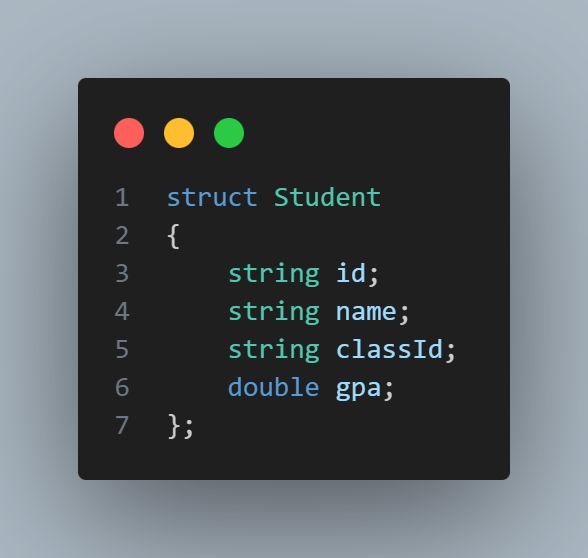
\includegraphics[width=0.45\textwidth]{code_student_struct.png}
\caption{Cấu trúc thực thể Student}
\label{fig:code_student_struct}
\end{figure}

\begin{figure}[htbp]
\centering
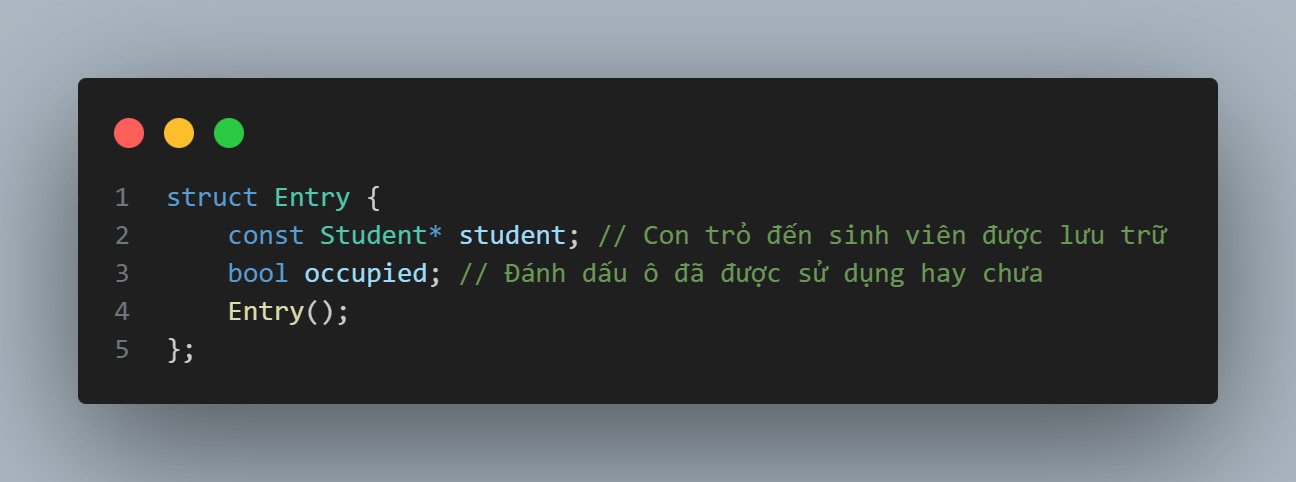
\includegraphics[width=0.68\textwidth]{code_entry_struct.png}
\caption{Cấu trúc ô nhớ Entry trong Bảng băm}
\label{fig:code_entry_struct}
\end{figure}

\subsubsection*{2.1.2. Hiện thực hàm băm chuỗi FNV-1a và phân bố giá trị băm}
\addcontentsline{toc}{subsubsection}{2.1.2. Hiện thực hàm băm chuỗi FNV-1a và phân bố giá trị băm}

Hàm băm đóng vai trò phân tán đều các khóa MSSV trên toàn bộ không gian bảng. Nhóm lựa chọn hàm băm FNV-1a (Fowler--Noll--Vo 1a) phiên bản 64-bit [6] vì ưu điểm cài đặt đơn giản, tốc độ tính toán nhanh trên chuỗi ký tự và cho độ phân tán tốt trên tập dữ liệu số báo danh sinh viên.

Thuật toán hoạt động dựa trên hai hằng số toán học nguyên tố theo đặc tả IETF [6]: hằng số bù ban đầu $\text{FNV\_OFFSET\_BASIS} = 14695981039346656037\text{ULL}$ và hằng số nguyên tố băm $\text{FNV\_PRIME} = 1099511628211\text{ULL}$. Quá trình băm duyệt tuần tự từng byte ký tự của chuỗi MSSV, thực hiện phép XOR bit với giá trị tích lũy hiện tại (\texttt{value \^{}= c}) rồi nhân với hằng số nguyên tố (\texttt{value *= FNV\_PRIME}).

\begin{figure}[htbp]
\centering
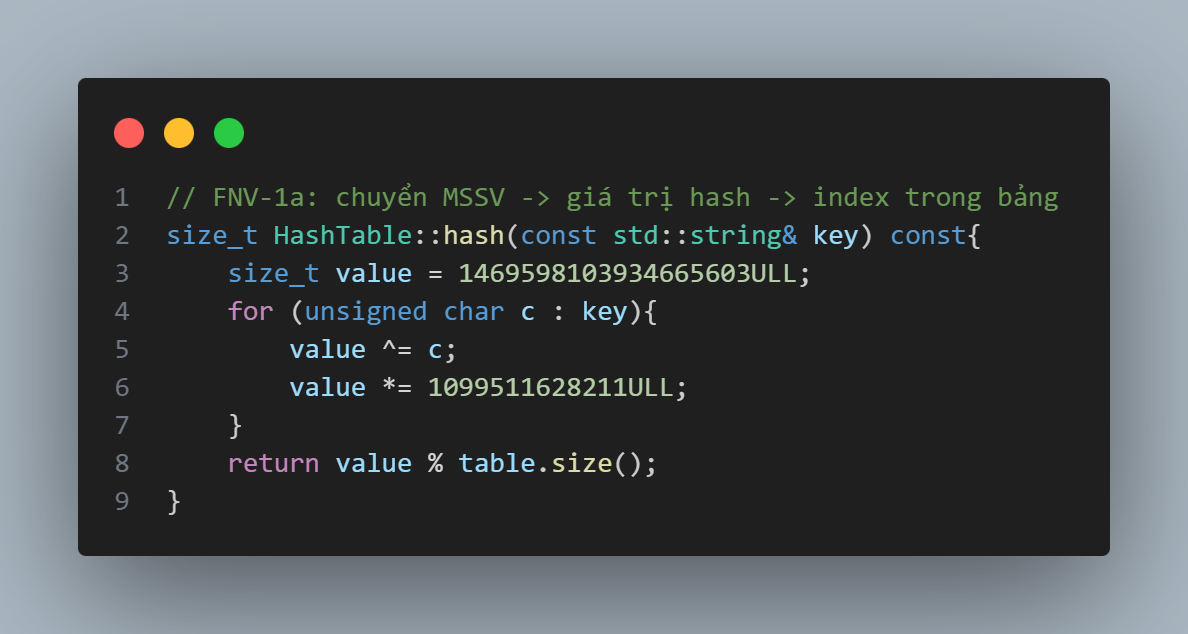
\includegraphics[width=0.65\textwidth]{code_fnv1a_hash.png}
\caption{Mã nguồn hàm băm chuỗi FNV-1a 64-bit tự cài đặt}
\label{fig:code_fnv1a_hash}
\end{figure}

Giá trị băm 64-bit đầu ra được ánh xạ vào chỉ số bảng thông qua phép chia lấy dư modulo với kích thước bảng $M = 2N + 1$. Cách chọn $M$ này nhằm duy trì hệ số tải xấp xỉ $0.5$, từ đó giảm số lần probe trung bình khi dò tuyến tính. Trong lần đo $10.000.000$ bản ghi, kích thước bảng thực tế là $20.000.001$ ô.

\subsubsection*{2.1.3. Cơ chế giải quyết đụng độ và thuật toán tìm kiếm}
\addcontentsline{toc}{subsubsection}{2.1.3. Cơ chế giải quyết đụng độ và thuật toán tìm kiếm}

Khi xảy ra hiện tượng đụng độ giữa hai khóa có cùng chỉ số ban đầu $h_0 = \text{hash}(\text{key}) \pmod M$, nhóm áp dụng giải thuật Dò tuyến tính (Linear Probing): $h_i = (h_0 + i) \pmod M$ với $i = 1, 2, \dots$. Phương pháp này lưu trữ toàn bộ các ô nhớ trên một mảng liên tục, tận dụng tính định vị không gian (Spatial Locality) của bộ đệm CPU Cache Line 64-byte [8].

Để duy trì hiệu năng trung bình tiệm cận $O(1)$, hệ số tải (\textit{Load Factor}) được kiểm soát ở mức $\alpha = N / M \approx 0.500$. Với benchmark hiện tại, $\alpha = 10.000.000 / 20.000.001 \approx 0.500$.

\begin{figure}[htbp]
\centering
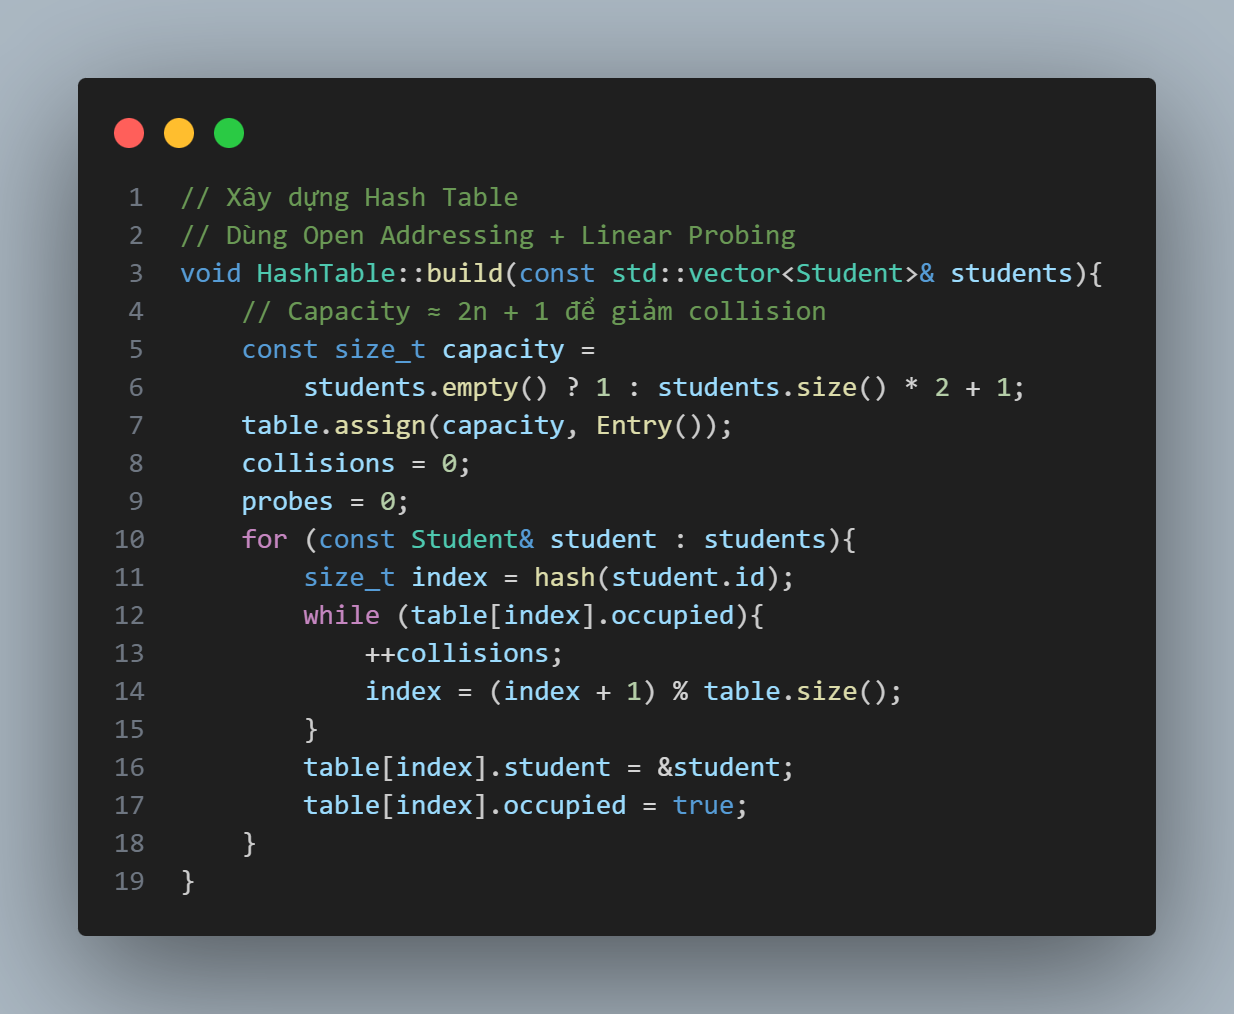
\includegraphics[width=0.65\textwidth]{code_hashtable_build.png}
\caption{Mã nguồn thuật toán nạp dữ liệu và xử lý đụng độ tuyến tính trong Bảng băm}
\label{fig:code_hashtable_build}
\end{figure}

Trong thuật toán xây dựng bảng (\texttt{build}), khi chèn một sinh viên, thuật toán tính chỉ số $h_0$ và tiến hành dò qua các ô nhớ kế tiếp cho đến khi gặp ô chưa bị chiếm (\texttt{!table[index].occupied}). Phần tử sau đó được gán trực tiếp vào ô trống này và bật cờ \texttt{occupied = true}.

Đối với thao tác tìm kiếm (\texttt{search}), giải thuật bắt đầu tại $h_0$ và duyệt qua các ô nhớ liên tiếp. Nếu gặp ô chưa chiếm (\texttt{!table[index].occupied}), thuật toán kết luận ngay khóa không tồn tại và trả về \texttt{nullptr}. Nếu gặp ô đã chiếm có mã sinh viên trùng khớp (\texttt{table[index].student->id == targetId}), hàm trả về con trỏ sinh viên tương ứng. Để đảm bảo an toàn, số bước dò được giới hạn tối đa không vượt quá kích thước bảng $M$.

\begin{figure}[htbp]
\centering
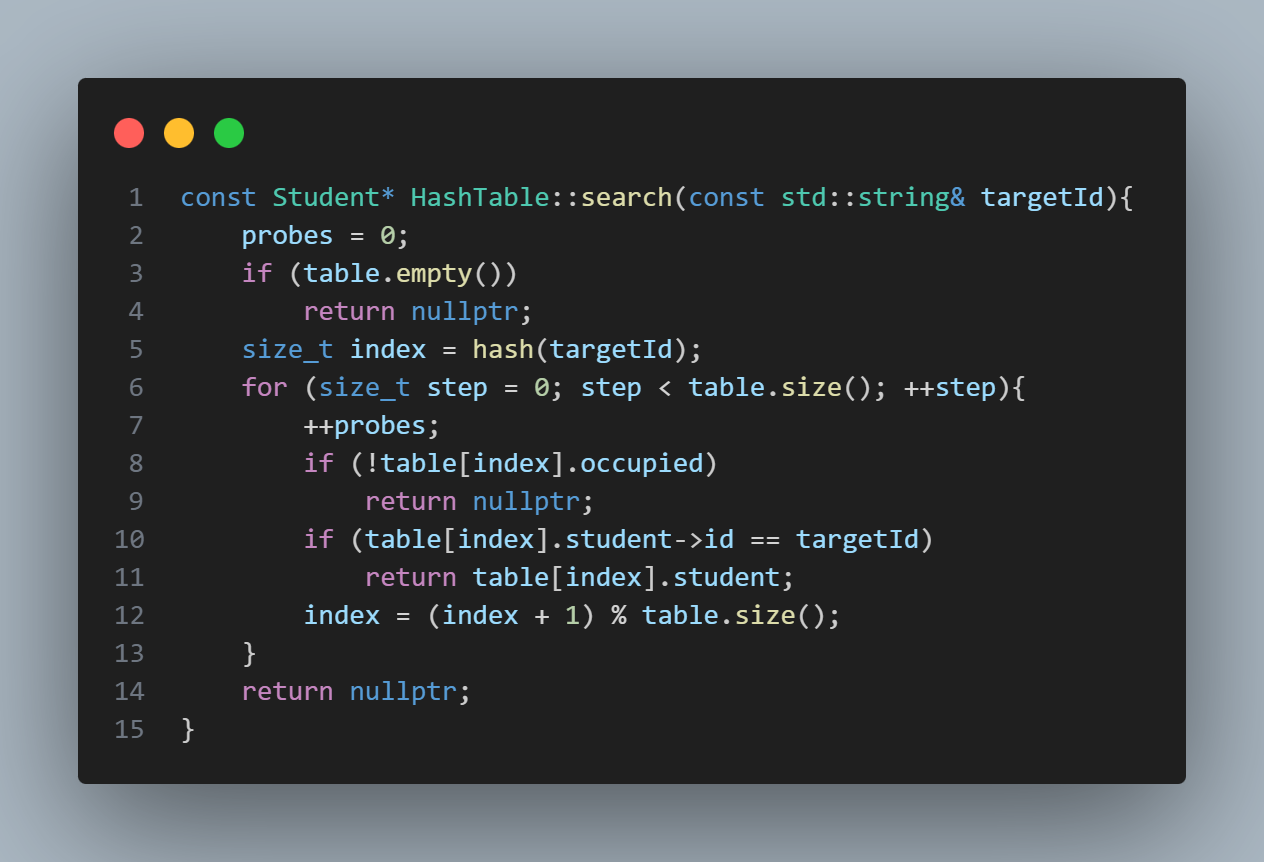
\includegraphics[width=0.65\textwidth]{code_hashtable_search.png}
\caption{Mã nguồn giải thuật tìm kiếm tra cứu chính xác theo MSSV trên Bảng băm}
\label{fig:code_hashtable_search}
\end{figure}

Luồng vận hành tra cứu chính xác theo MSSV (Yêu cầu MC1) được mô hình hóa trong Sơ đồ tuần tự Hình \ref{fig:seq_mc1_lookup}. Toàn bộ tiến trình gồm: tiếp nhận MSSV từ giao diện Web, chuyển qua API Bridge, thực hiện tra cứu trên Bảng băm đóng bằng FNV-1a và Linear Probing trong thời gian trung bình $O(1)$, sau đó chuyển đổi kết quả thành JSON trả về giao diện.

\begin{figure}[htbp]
\centering
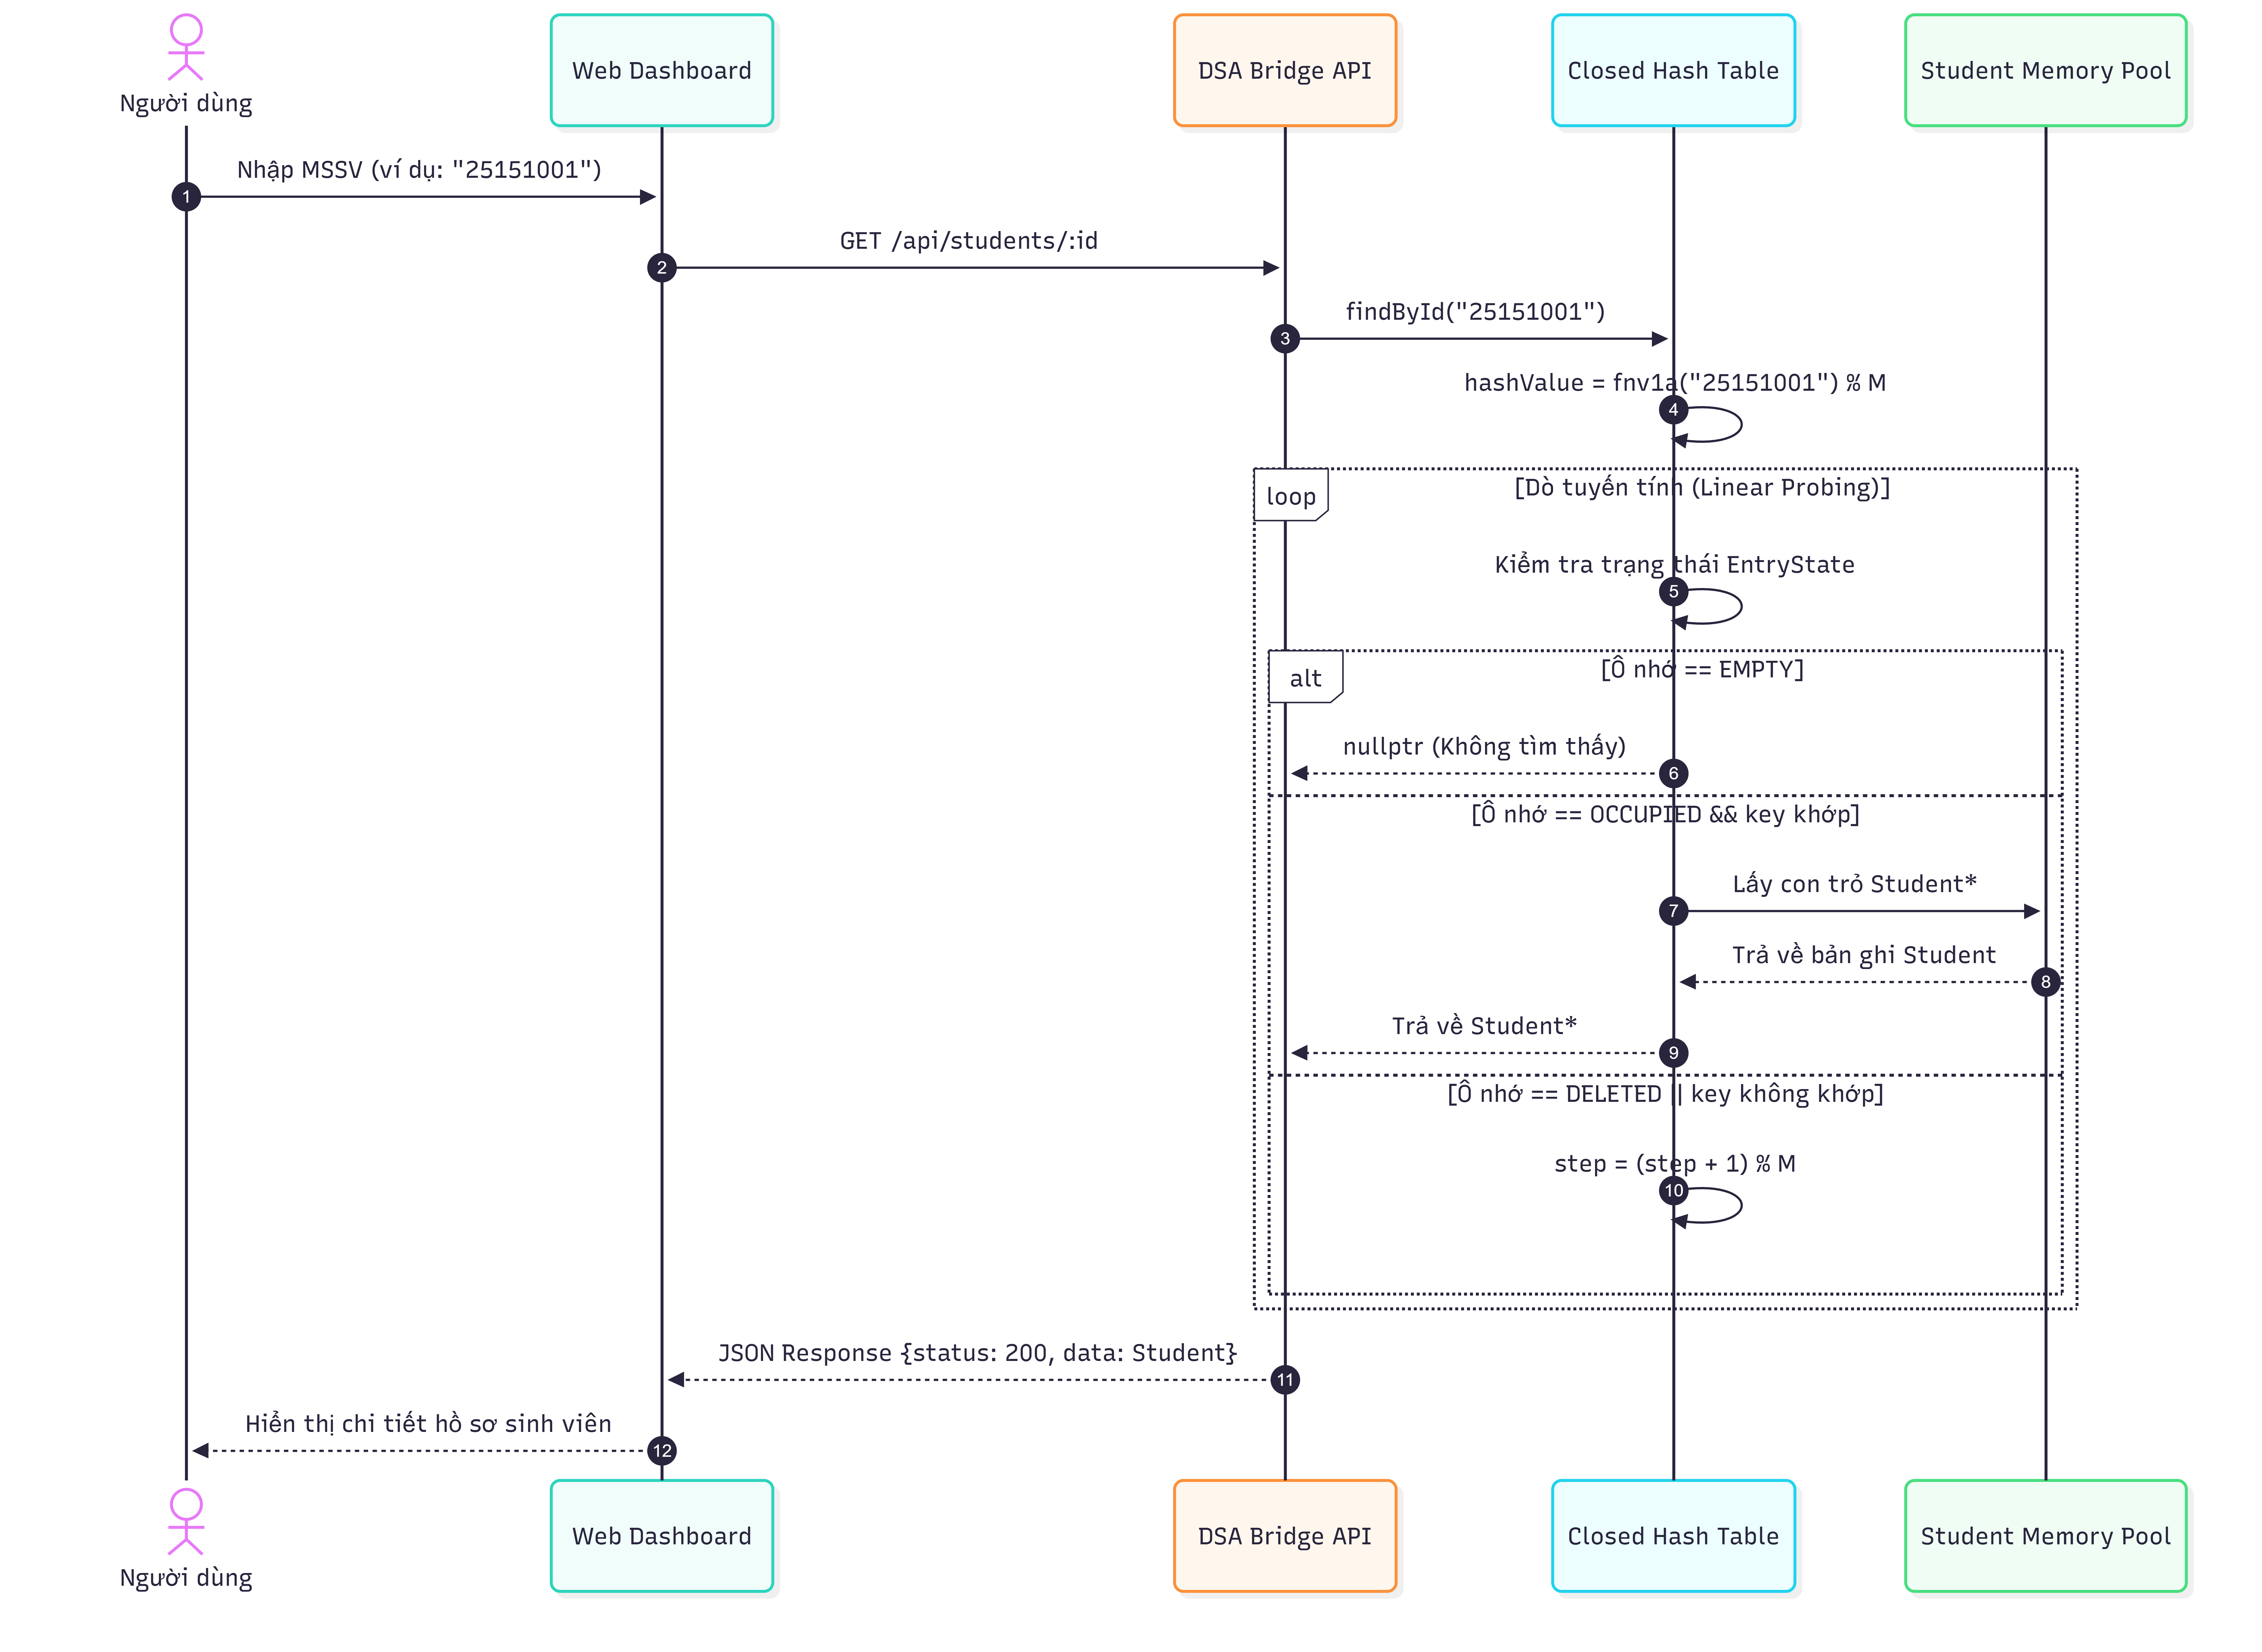
\includegraphics[width=0.70\textwidth]{seq_mc1_lookup.png}
\caption{Sơ đồ tuần tự (Sequence Diagram) luồng tra cứu chính xác theo MSSV trên Bảng băm}
\label{fig:seq_mc1_lookup}
\end{figure}

\subsubsection*{2.1.4. Phân tích chi phí thời gian và không gian bộ nhớ}
\addcontentsline{toc}{subsubsection}{2.1.4. Phân tích chi phí thời gian và không gian bộ nhớ}

Theo phân tích của Donald E. Knuth [2], với Bảng băm đóng sử dụng dò tuyến tính khi duy trì hệ số tải thấp $\alpha = N / M \approx 0.50$, số bước thăm dò trung bình kỳ vọng cho mỗi thao tác tra cứu là rất nhỏ: chỉ khoảng $1.50$ lần truy cập đối với tìm kiếm thành công và $2.50$ lần đối với tìm kiếm không thành công.

Điều này giải thích vì sao chi phí tìm kiếm trung bình của Bảng băm đóng luôn đạt mức hằng số $O(1)$ độc lập với quy mô dữ liệu $N$. Trong trường hợp xấu nhất về mặt lý thuyết (khi xảy ra hiện tượng đụng độ dồn cục bộ cực đoan -- Primary Clustering), chi phí có thể tăng lên $O(M)$ [1], [2]. Tuy nhiên, trong thực tế hệ thống đã kiểm soát triệt để rủi ro này nhờ phân bố đều của hàm băm FNV-1a kết hợp với việc giữ bảng luôn thưa ở mức $\alpha \approx 0.50$. Về không gian bộ nhớ, mỗi ô \texttt{Entry} chiếm $16$ bytes gồm một con trỏ \texttt{Student*} (8 bytes) và cờ trạng thái cùng vùng đệm căn lề (8 bytes). Với benchmark $10.000.000$ bản ghi, bảng $20.000.001$ ô tiêu tốn khoảng $320$ MB RAM trên một mảng phẳng liên tục, tương thích với các dòng Cache Line $64$-byte của vi xử lý hiện đại.

\subsection*{2.2. Cài đặt chi tiết cấu trúc Cây đống cực đại từ đầu (From Scratch 2)}
\addcontentsline{toc}{subsection}{2.2. Cài đặt chi tiết cấu trúc Cây đống cực đại từ đầu (From Scratch 2)}

\subsubsection*{2.2.1. Biểu diễn mảng phẳng 1 chiều và công thức truy xuất chỉ số nút}
\addcontentsline{toc}{subsubsection}{2.2.1. Biểu diễn mảng phẳng 1 chiều và công thức truy xuất chỉ số nút}

Cấu trúc Cây đống cực đại (Custom Binary Max-Heap) được nhóm cài đặt trên mảng 1 chiều liên tục \texttt{std::vector<Student>} với gốc đặt tại chỉ số $0$. Code hiện tại sao chép dữ liệu từ vector gốc vào \texttt{maxHeap}, sau đó áp dụng Floyd Build Heap. Cách tổ chức này tránh các node cây cấp phát rời rạc, cho phép chuyển đổi quan hệ cha--con thành các phép tính chỉ số đơn giản:
Nút con bên trái của nút tại chỉ số $i$ được tính theo công thức $\text{leftChild}(i) = 2i + 1$; nút con bên phải được tính theo công thức $\text{rightChild}(i) = 2i + 2$; và nút cha được tính theo công thức $\text{parent}(i) = \lfloor (i - 1) / 2 \rfloor$.

Các thao tác xác định chỉ số này được thực hiện bằng các phép toán số học có chi phí $O(1)$, mang lại tốc độ truy xuất nhanh và tận dụng tối đa tính liên tục của bộ nhớ RAM.

\subsubsection*{2.2.2. Hiện thực thuật toán vun đống Floyd Build Heap trong thời gian \texorpdfstring{$O(N)$}{O(N)}}
\addcontentsline{toc}{subsubsection}{2.2.2. Hiện thực thuật toán vun đống Floyd Build Heap trong thời gian \texorpdfstring{$O(N)$}{O(N)}}

Thay vì chèn lần lượt từng sinh viên vào đống với chi phí $O(N \log N)$, nhóm hiện thực thuật toán vun đống từ dưới lên cổ điển của Robert W. Floyd (\textit{Floyd Bottom-up Build Heap}). Thuật toán khởi đầu bằng việc sao chép/nạp toàn bộ $N$ bản ghi \texttt{Student} vào mảng \texttt{maxHeap}, sau đó tiến hành duyệt ngược từ nút cha cuối cùng không phải là lá tại vị trí $i = \lfloor N/2 \rfloor - 1$ lùi dần về nút gốc tại vị trí $i = 0$, gọi hàm \texttt{heapifyDown(i)} tại mỗi bước.

\begin{figure}[htbp]
\centering
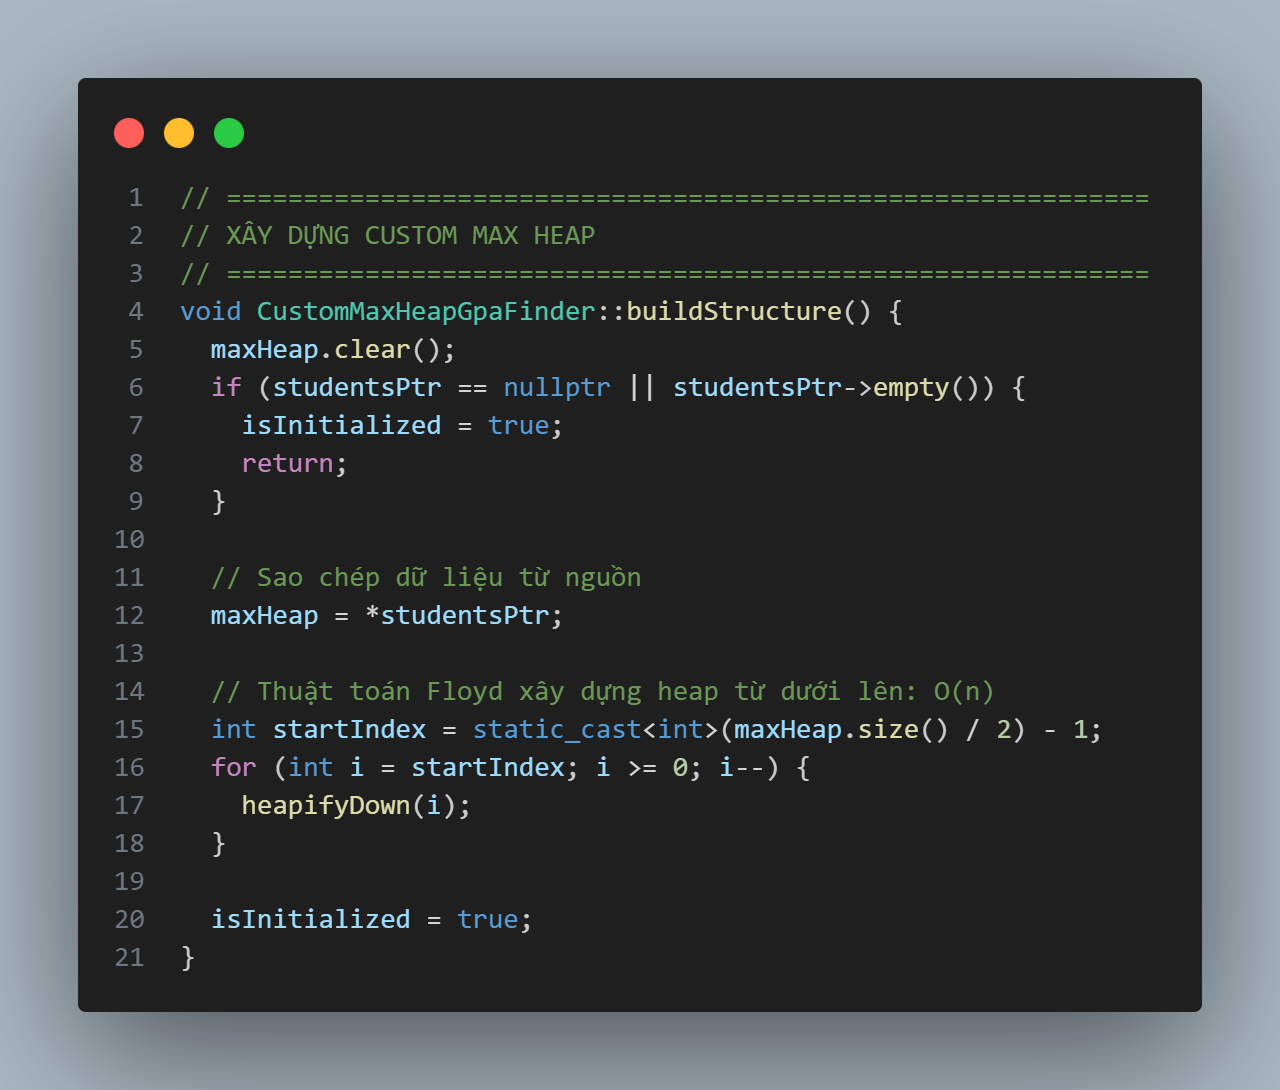
\includegraphics[width=0.65\textwidth]{code_floyd_build_heap.png}
\caption{Mã nguồn thuật toán Floyd Build Heap O(N) tự cài đặt}
\label{fig:code_floyd_build_heap}
\end{figure}

Về mặt bản chất, lý do thuật toán Floyd Build Heap khởi chạy từ chỉ số $i = \lfloor N/2 \rfloor - 1$ thay vì duyệt từ phần tử cuối cùng $N-1$ xuất phát từ đặc tính phân tầng của cây nhị phân hoàn chỉnh:

\textbf{Tầng nút lá:} Khoảng một nửa số nút (tất cả các nút có chỉ số từ $\lfloor N/2 \rfloor$ đến $N-1$) là các nút lá. Mỗi nút lá không có nút con nên tự thân đã thỏa mãn tính chất Max-Heap, do đó hệ thống hoàn toàn không cần thực hiện \texttt{heapifyDown} cho các nút này.

\textbf{Tầng cận lá:} Phần lớn các nút nội vi còn lại nằm rất gần tầng lá, nên chỉ cần tối đa 1 đến 2 bước đổi chỗ để ổn định vị trí.

\textbf{Tầng gần gốc:} Chỉ có rất ít nút nằm gần gốc mới có khả năng phải di chuyển qua nhiều tầng (với chiều cao tối đa $\lfloor \log_2 N \rfloor$).

Nhờ phần lớn công việc chỉ tập trung ở các nút tầng thấp với số phép hoán vị rất ít, tổng khối lượng xử lý của thuật toán Floyd Build Heap tăng tuyến tính theo số phần tử, đạt độ phức tạp $O(N)$. Trong khi đó, nếu xây dựng Heap bằng cách chèn tuần tự từng phần tử từ trên xuống, mỗi lần chèn có thể mất $O(\log N)$ dẫn đến tổng chi phí $O(N \log N)$. Vì vậy, Floyd Build Heap là giải pháp vượt trội và phù hợp nhất cho giai đoạn Bulk Load dữ liệu quy mô lớn.

Cốt lõi của tiến trình vun đống là giải thuật \texttt{heapifyDown} được cài đặt thông qua vòng lặp \texttt{while (true)} dạng lặp (iterative) nhằm tránh chi phí gọi hàm đệ quy (\textit{Function Call Overhead}) và giúp việc quản lý, cập nhật chỉ số nút trực tiếp, tường minh hơn. Với một cây nhị phân hoàn chỉnh gồm $10.000.000$ phần tử, chiều cao tối đa của đống chỉ khoảng $\lfloor \log_2 N \rfloor \approx 23$ tầng. Tại mỗi bước lặp, hàm xác định chỉ số con trái $\text{left} = 2 \times \text{index} + 1$ và con phải $\text{right} = 2 \times \text{index} + 2$. Biến \texttt{highest} ban đầu được gán là nút hiện tại (\texttt{index}). Thuật toán lần lượt kiểm tra điều kiện chỉ số hợp lệ trong phạm vi mảng và gọi hàm so sánh ưu tiên \texttt{higherPriority} để tìm ra nút có độ ưu tiên cao nhất trong bộ ba: nút cha, nút con trái và nút con phải. Nếu nút cha đã có độ ưu tiên lớn hơn hoặc bằng cả hai con (\texttt{highest == index}), cấu trúc đống tại vị trí này đã thỏa mãn bất biến Max-Heap và vòng lặp dừng. Ngược lại, nếu một trong hai nút con có độ ưu tiên cao hơn, hàm thực hiện hoán vị hai bản ghi \texttt{Student} bằng \texttt{std::swap}, cập nhật \texttt{index = highest} và tiếp tục duyệt xuống các tầng bên dưới.

\begin{figure}[htbp]
\centering
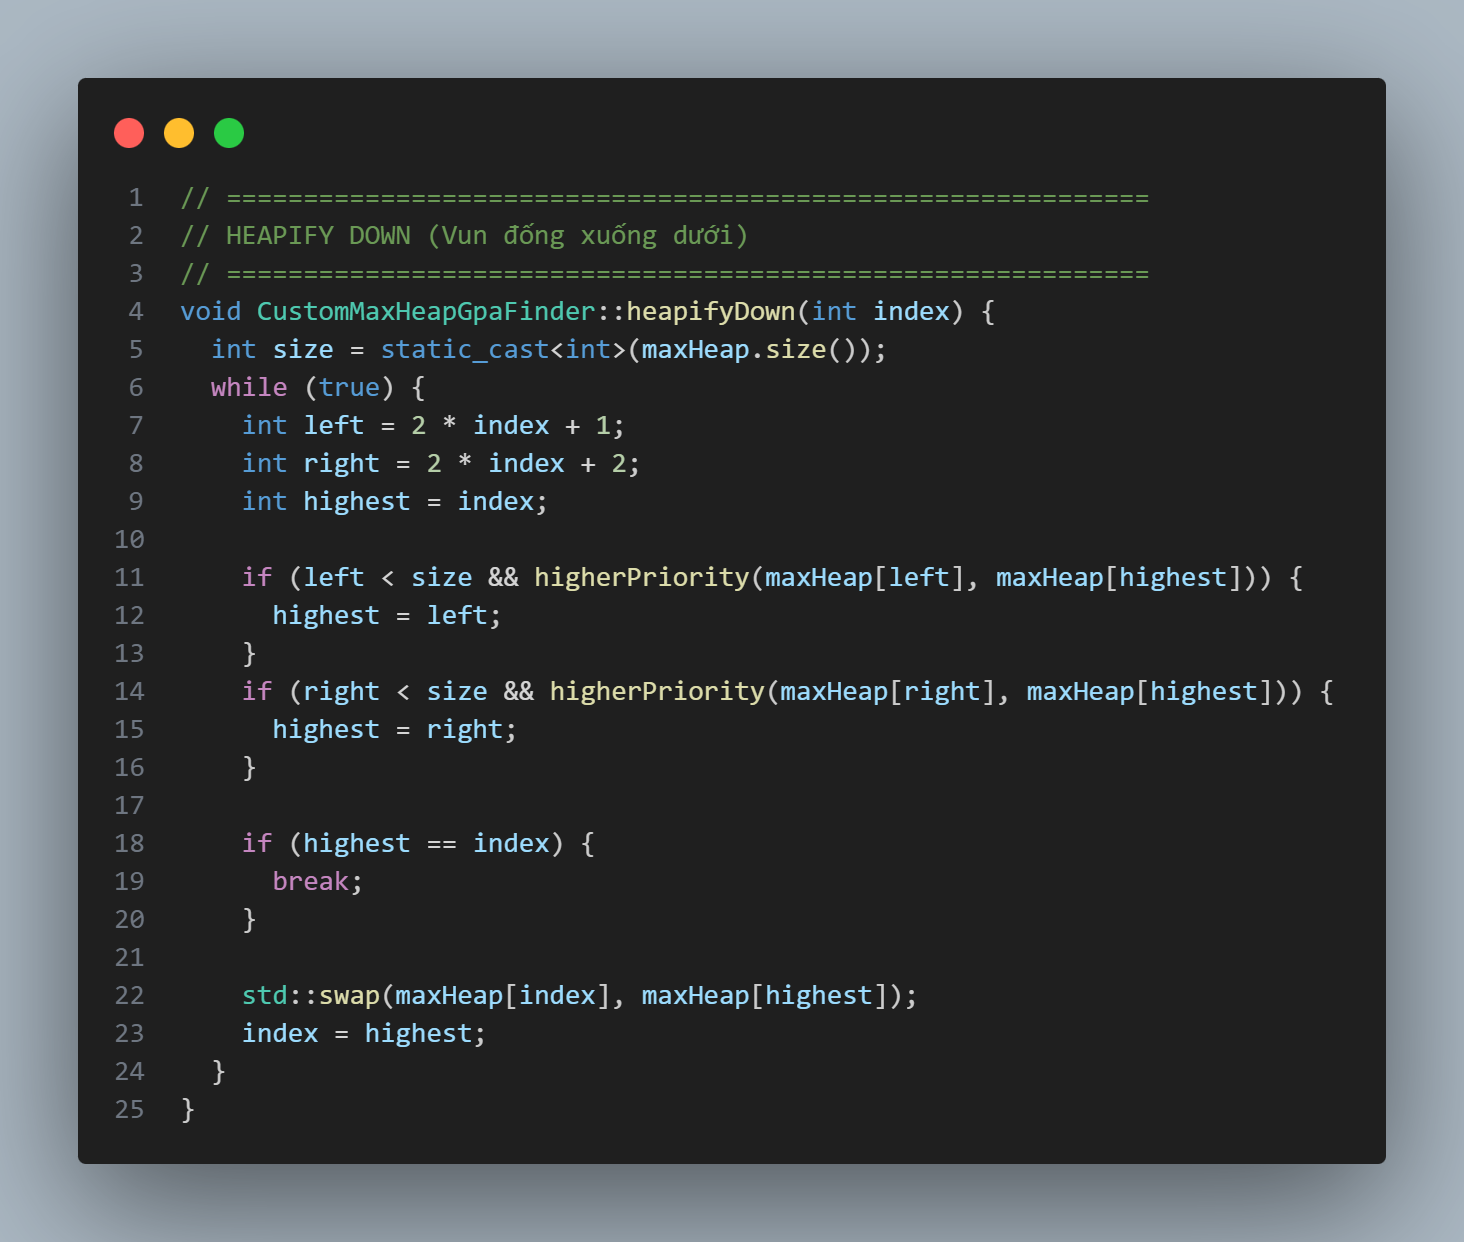
\includegraphics[width=0.65\textwidth]{code_heapify_down.png}
\caption{Mã nguồn hàm heapifyDown duy trì bất biến cấu trúc Max-Heap}
\label{fig:code_heapify_down}
\end{figure}

\subsubsection*{2.2.3. Cài đặt các thao tác truy xuất cực trị và cập nhật đống}
\addcontentsline{toc}{subsubsection}{2.2.3. Cài đặt các thao tác truy xuất cực trị và cập nhật đống}

Cấu trúc Max-Heap cung cấp các thao tác cơ bản với độ phức tạp phân định rõ ràng:
\textbf{Truy xuất phần tử lớn nhất (\texttt{peekMax}):} Chỉ đọc bản ghi \texttt{Student} tại vị trí gốc \texttt{maxHeap[0]} với chi phí thời gian $O(1)$ [1].

\textbf{Lấy và xóa phần tử lớn nhất (\texttt{extractMax}):} Hoán vị phần tử gốc với phần tử cuối cùng ở đáy mảng, giảm kích thước đống đi 1 và thực hiện \texttt{heapifyDown(0)} để phục hồi tính chất đống với chi phí $O(\log N)$ [1], [5].

\textbf{Chèn phần tử mới (\texttt{insert}):} Đẩy phần tử vào cuối mảng và thực hiện thao tác vun đống ngược lên (\texttt{heapifyUp}) qua các nút cha với thời gian $O(\log N)$.

Luồng vận hành truy xuất GPA cao nhất (Yêu cầu MC2) được mô hình hóa chi tiết trong Sơ đồ tuần tự Hình \ref{fig:seq_mc2_extreme}. Tiến trình gồm: nhận yêu cầu từ Web Dashboard, API Bridge gọi tầng C++ Core, đọc trực tiếp bản ghi tại gốc \texttt{maxHeap[0]} trong thời gian $O(1)$, và đóng gói JSON phản hồi về giao diện.

\begin{figure}[htbp]
\centering
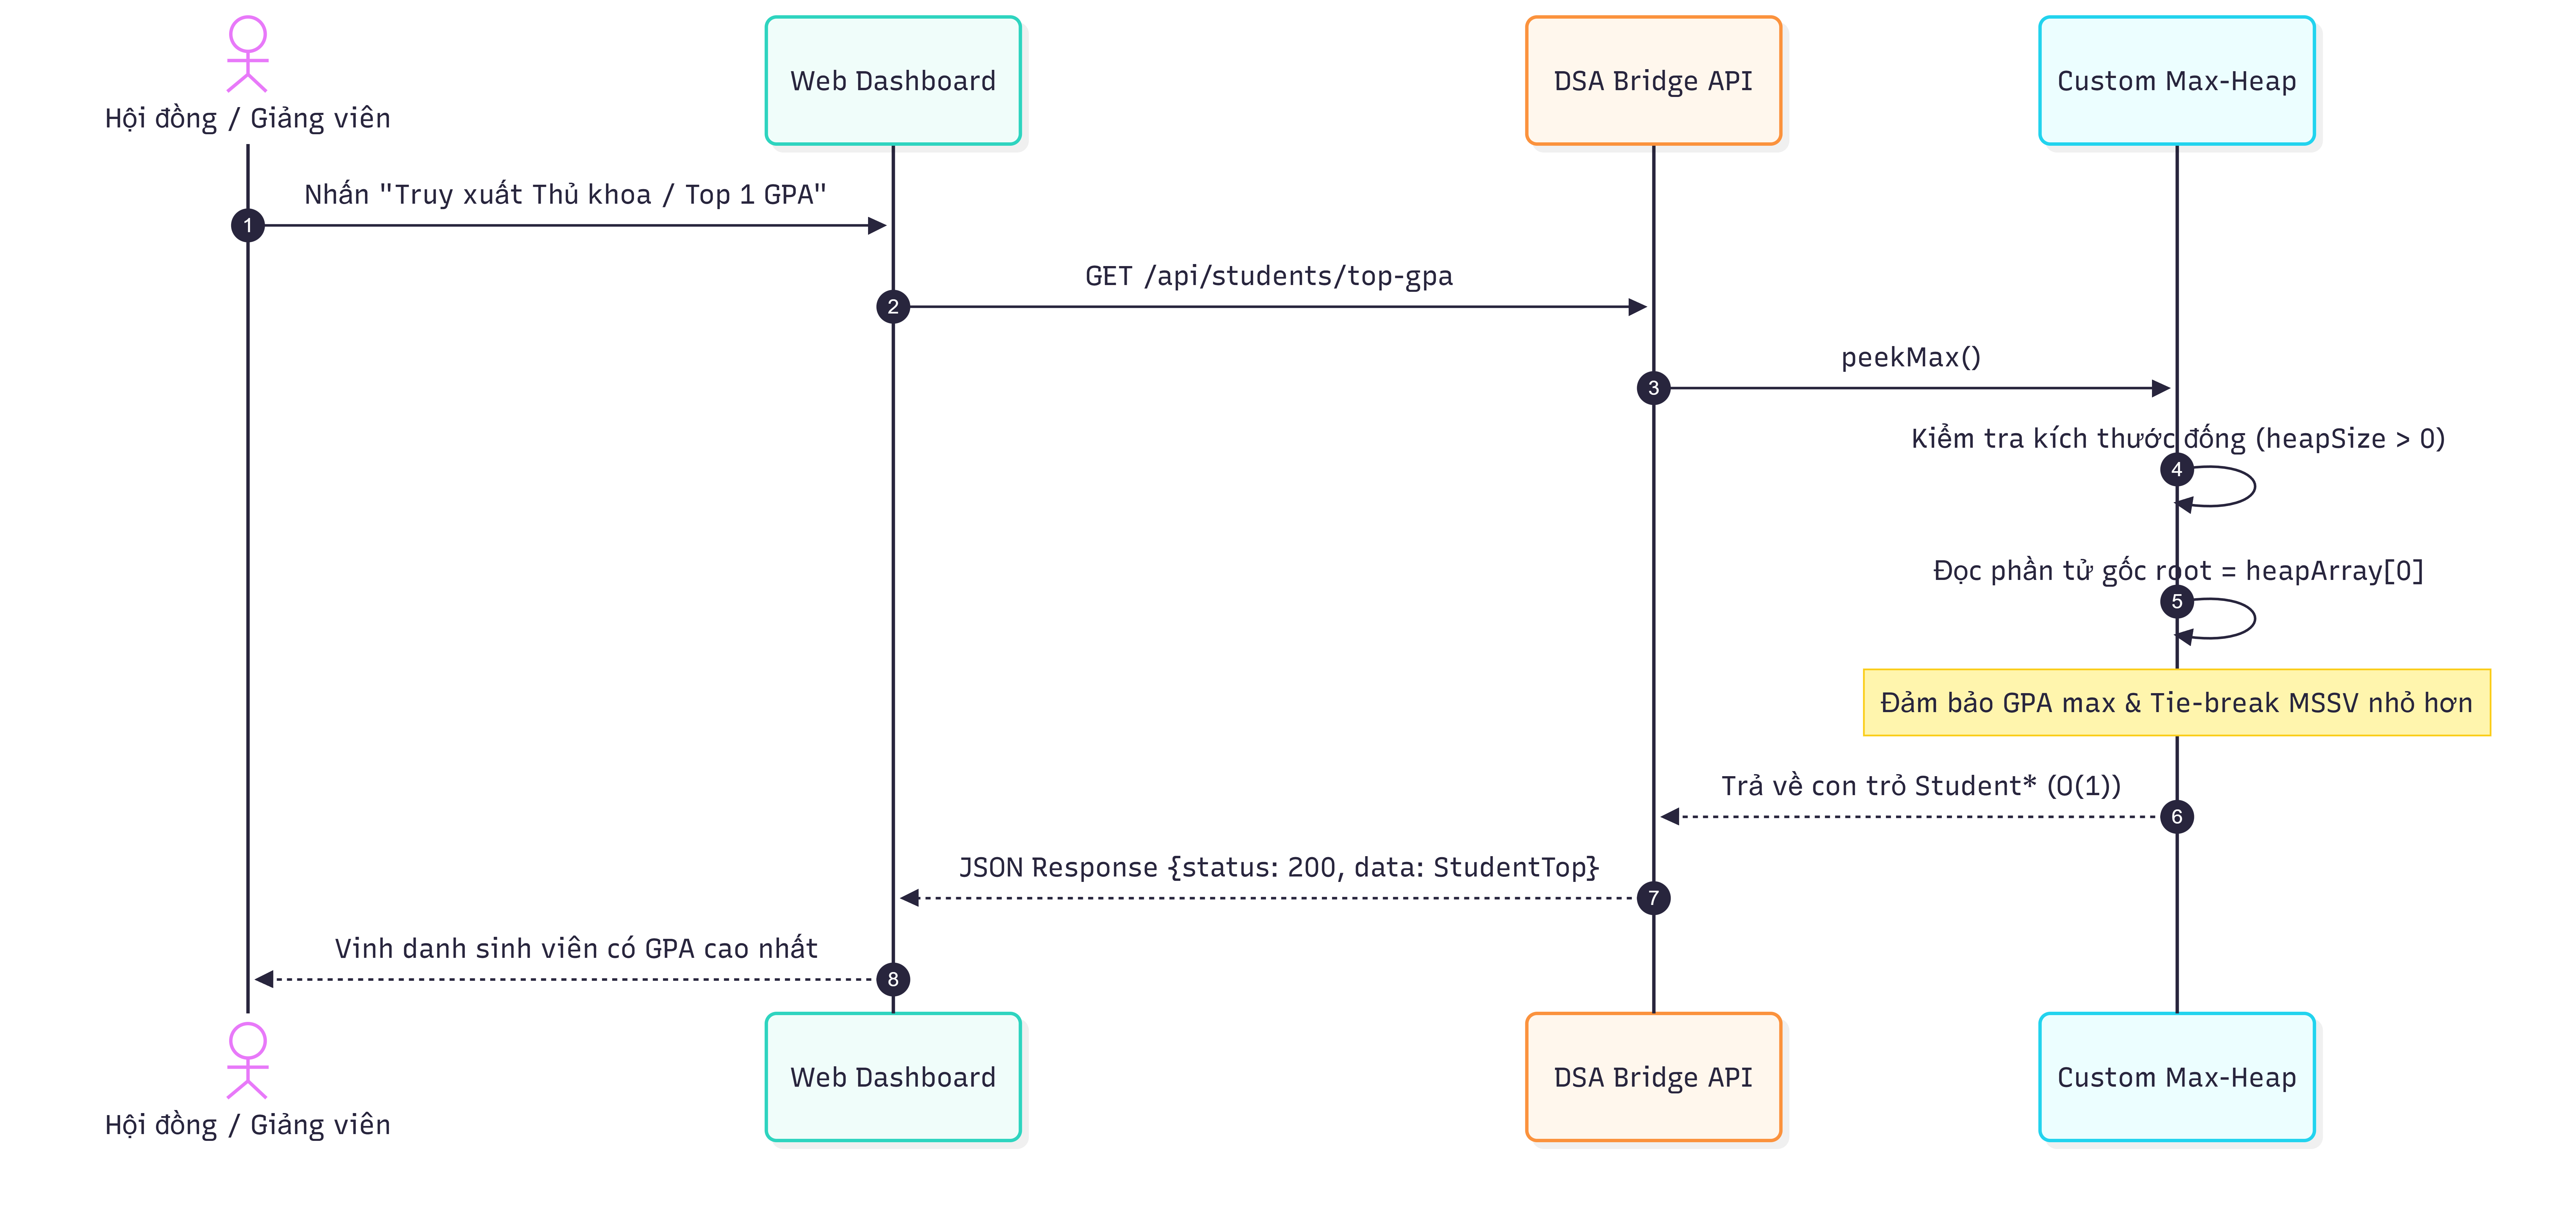
\includegraphics[width=0.76\textwidth]{seq_mc2_extreme.png}
\caption{Sơ đồ tuần tự (Sequence Diagram) luồng trích xuất GPA cao nhất trên Max-Heap}
\label{fig:seq_mc2_extreme}
\end{figure}

\subsubsection*{2.2.4. Xử lý quy tắc phân định đồng hạng (Tie-breaking Rule)}
\addcontentsline{toc}{subsubsection}{2.2.4. Xử lý quy tắc phân định đồng hạng (Tie-breaking Rule)}

Trên tập dữ liệu thực nghiệm hiện tại $10.000.000$ sinh viên, số lượng sinh viên có cùng mức điểm GPA có thể rất lớn. Để đảm bảo tính xác định và nhất quán của kết quả đầu ra, nhóm cài đặt hàm so sánh ưu tiên \texttt{higherPriority(a, b)} theo quy tắc rõ ràng: sinh viên $a$ có độ ưu tiên cao hơn $b$ khi và chỉ khi $a.\text{gpa} > b.\text{gpa}$, hoặc trong trường hợp hai sinh viên có cùng điểm GPA ($a.\text{gpa} == b.\text{gpa}$) thì sinh viên có mã số nhỏ hơn ($a.\text{id} < b.\text{id}$) theo thứ tự từ điển sẽ được xếp trước.

\begin{figure}[htbp]
\centering
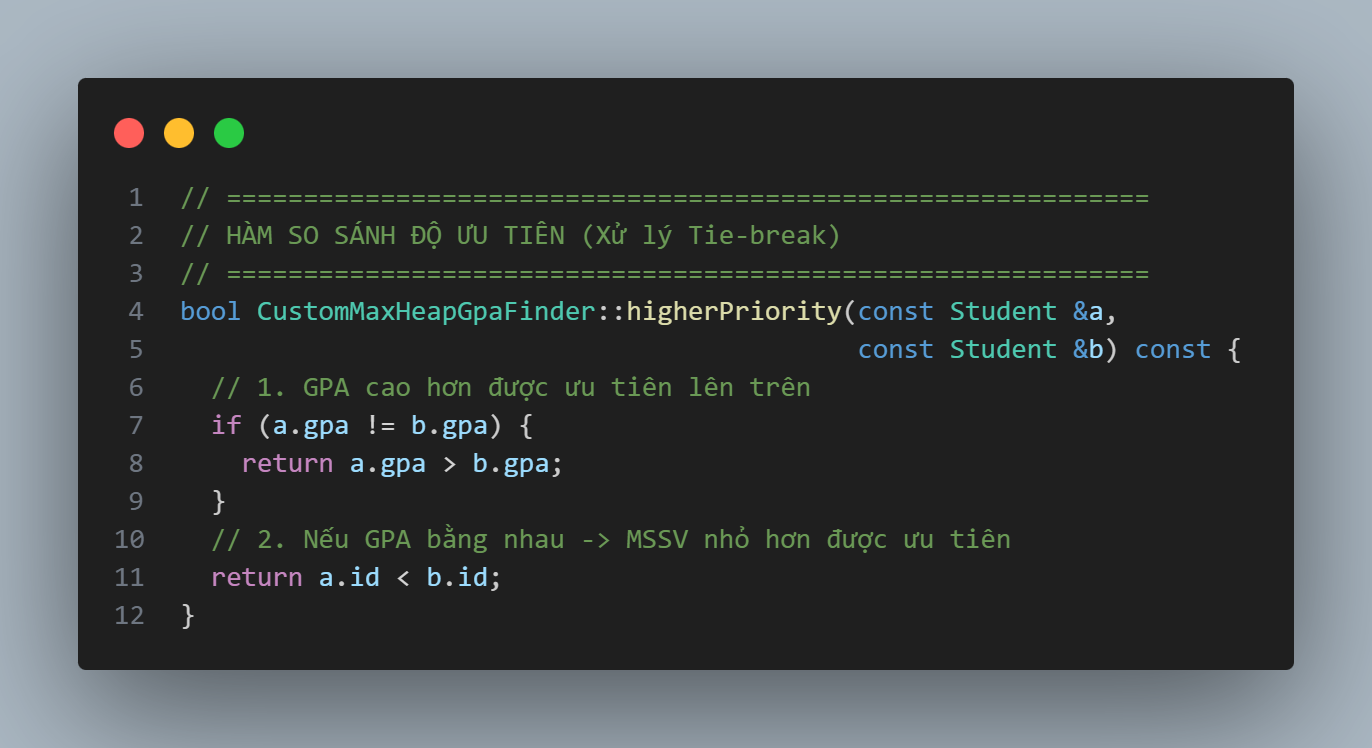
\includegraphics[width=0.72\textwidth]{code_heap_tiebreak.png}
\caption{Hiện thực toán tử phân định đồng hạng kết hợp GPA và MSSV}
\label{fig:code_heap_tiebreak}
\end{figure}

Quy tắc này đảm bảo rằng sinh viên có GPA cao hơn luôn đứng trước; nếu hai sinh viên có cùng điểm GPA thì sinh viên có mã số sinh viên nhỏ hơn theo thứ tự từ điển sẽ được ưu tiên đứng tại vị trí nút gốc.

\subsection*{2.3. Cài đặt các thuật toán bổ trợ và xử lý Range Query}
\addcontentsline{toc}{subsection}{2.3. Cài đặt các thuật toán bổ trợ và xử lý Range Query}

\subsubsection*{2.3.1. Xây dựng mảng dữ liệu sắp xếp theo điểm GPA (RQ2)}
\addcontentsline{toc}{subsubsection}{2.3.1. Xây dựng mảng dữ liệu sắp xếp theo điểm GPA (RQ2)}

Để phục vụ yêu cầu truy vấn theo khoảng điểm GPA (RQ2), module \texttt{SortedGpaFilter} duy trì một mảng con trỏ \texttt{vector<const Student*> sortedStudents}. Mỗi phần tử trong mảng này trỏ về một bản ghi trong \texttt{vector<Student>} gốc, sau đó toàn bộ mảng con trỏ được sắp xếp theo thứ tự điểm GPA tăng dần thông qua \texttt{std::sort} với toán tử so sánh lambda tùy biến theo trường \texttt{gpa}. Cách tổ chức này tránh sao chép bản ghi \texttt{Student}, giảm footprint của chỉ mục GPA xuống còn chi phí con trỏ, đồng thời vẫn cho phép truy cập trực tiếp bản ghi thật khi cần hiển thị. Trong môi trường GCC/MinGW-w64 của nhóm, \texttt{std::sort} vận hành với chi phí thời gian trung bình $O(N \log N)$ [1], [7].

\begin{figure}[htbp]
\centering
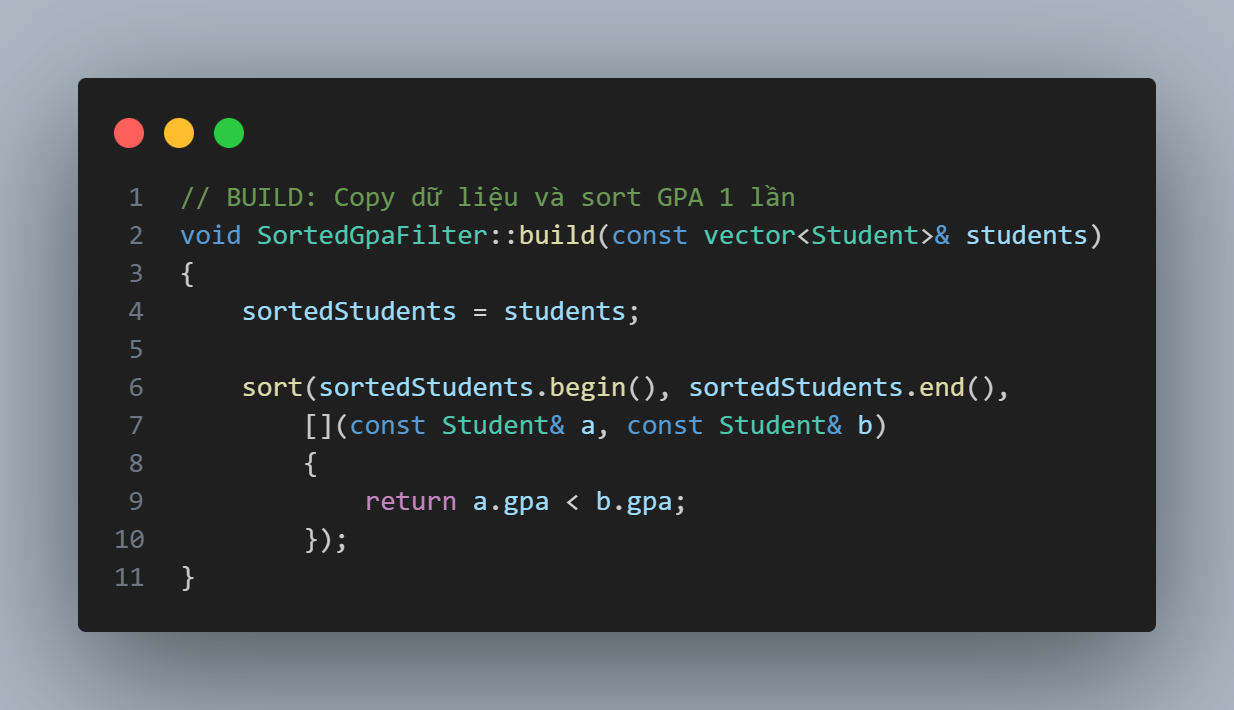
\includegraphics[width=0.70\textwidth]{code_sorted_gpa_build.png}
\caption{Mã nguồn xây dựng mảng dữ liệu sắp xếp theo GPA phục vụ Range Query}
\label{fig:code_sorted_gpa_build}
\end{figure}

\subsubsection*{2.3.2. Hiện thực thuật toán tìm kiếm nhị phân 2 đầu biên trên mảng sắp xếp}
\addcontentsline{toc}{subsubsection}{2.3.2. Hiện thực thuật toán tìm kiếm nhị phân 2 đầu biên trên mảng sắp xếp}

Bài toán truy vấn theo dải điểm $[\text{minGPA}, \text{maxGPA}]$ đòi hỏi phải xác định chính xác hai vị trí biên trong mảng đã sắp xếp mà không được quét tuần tự toàn mảng ($O(N)$). Trên tập benchmark hiện tại $10.000.000$ phần tử, lợi ích của tìm kiếm nhị phân thể hiện rõ khi so với quét tuyến tính toàn mảng. Nhóm tự cài đặt thuật toán Tìm kiếm nhị phân hai đầu biên (\textit{Dual-boundary Binary Search}) với hai bước tìm kiếm độc lập: tìm kiếm biên dưới (\textit{Lower Bound}) và tìm kiếm biên trên (\textit{Upper Bound}).

Về mặt giải thuật, hàm tìm kiếm biên dưới duyệt không gian tìm kiếm $[0, N)$ bằng cách chia đôi đoạn khảo sát. Tại mỗi bước lặp với $\text{mid} = \text{left} + (\text{right} - \text{left}) / 2$, nếu \texttt{sortedStudents[mid]->gpa < minGPA}, đoạn tìm kiếm được thu hẹp về nửa bên phải ($\text{left} = \text{mid} + 1$); ngược lại, $\text{right} = \text{mid}$. Vòng lặp dừng khi $\text{left} == \text{right}$, trả về vị trí phần tử đầu tiên có $\text{gpa} \ge \text{minGPA}$ (chỉ số \texttt{startIndex}) trong thời gian $O(\log N)$. Tương tự, hàm tìm kiếm biên trên sử dụng điều kiện \texttt{sortedStudents[mid]->gpa <= maxGPA} để xác định vị trí đầu tiên có điểm GPA nghiêm ngặt lớn hơn \texttt{maxGPA} (chỉ số \texttt{endIndex}) cũng trong thời gian $O(\log N)$.

\begin{figure}[htbp]
\centering
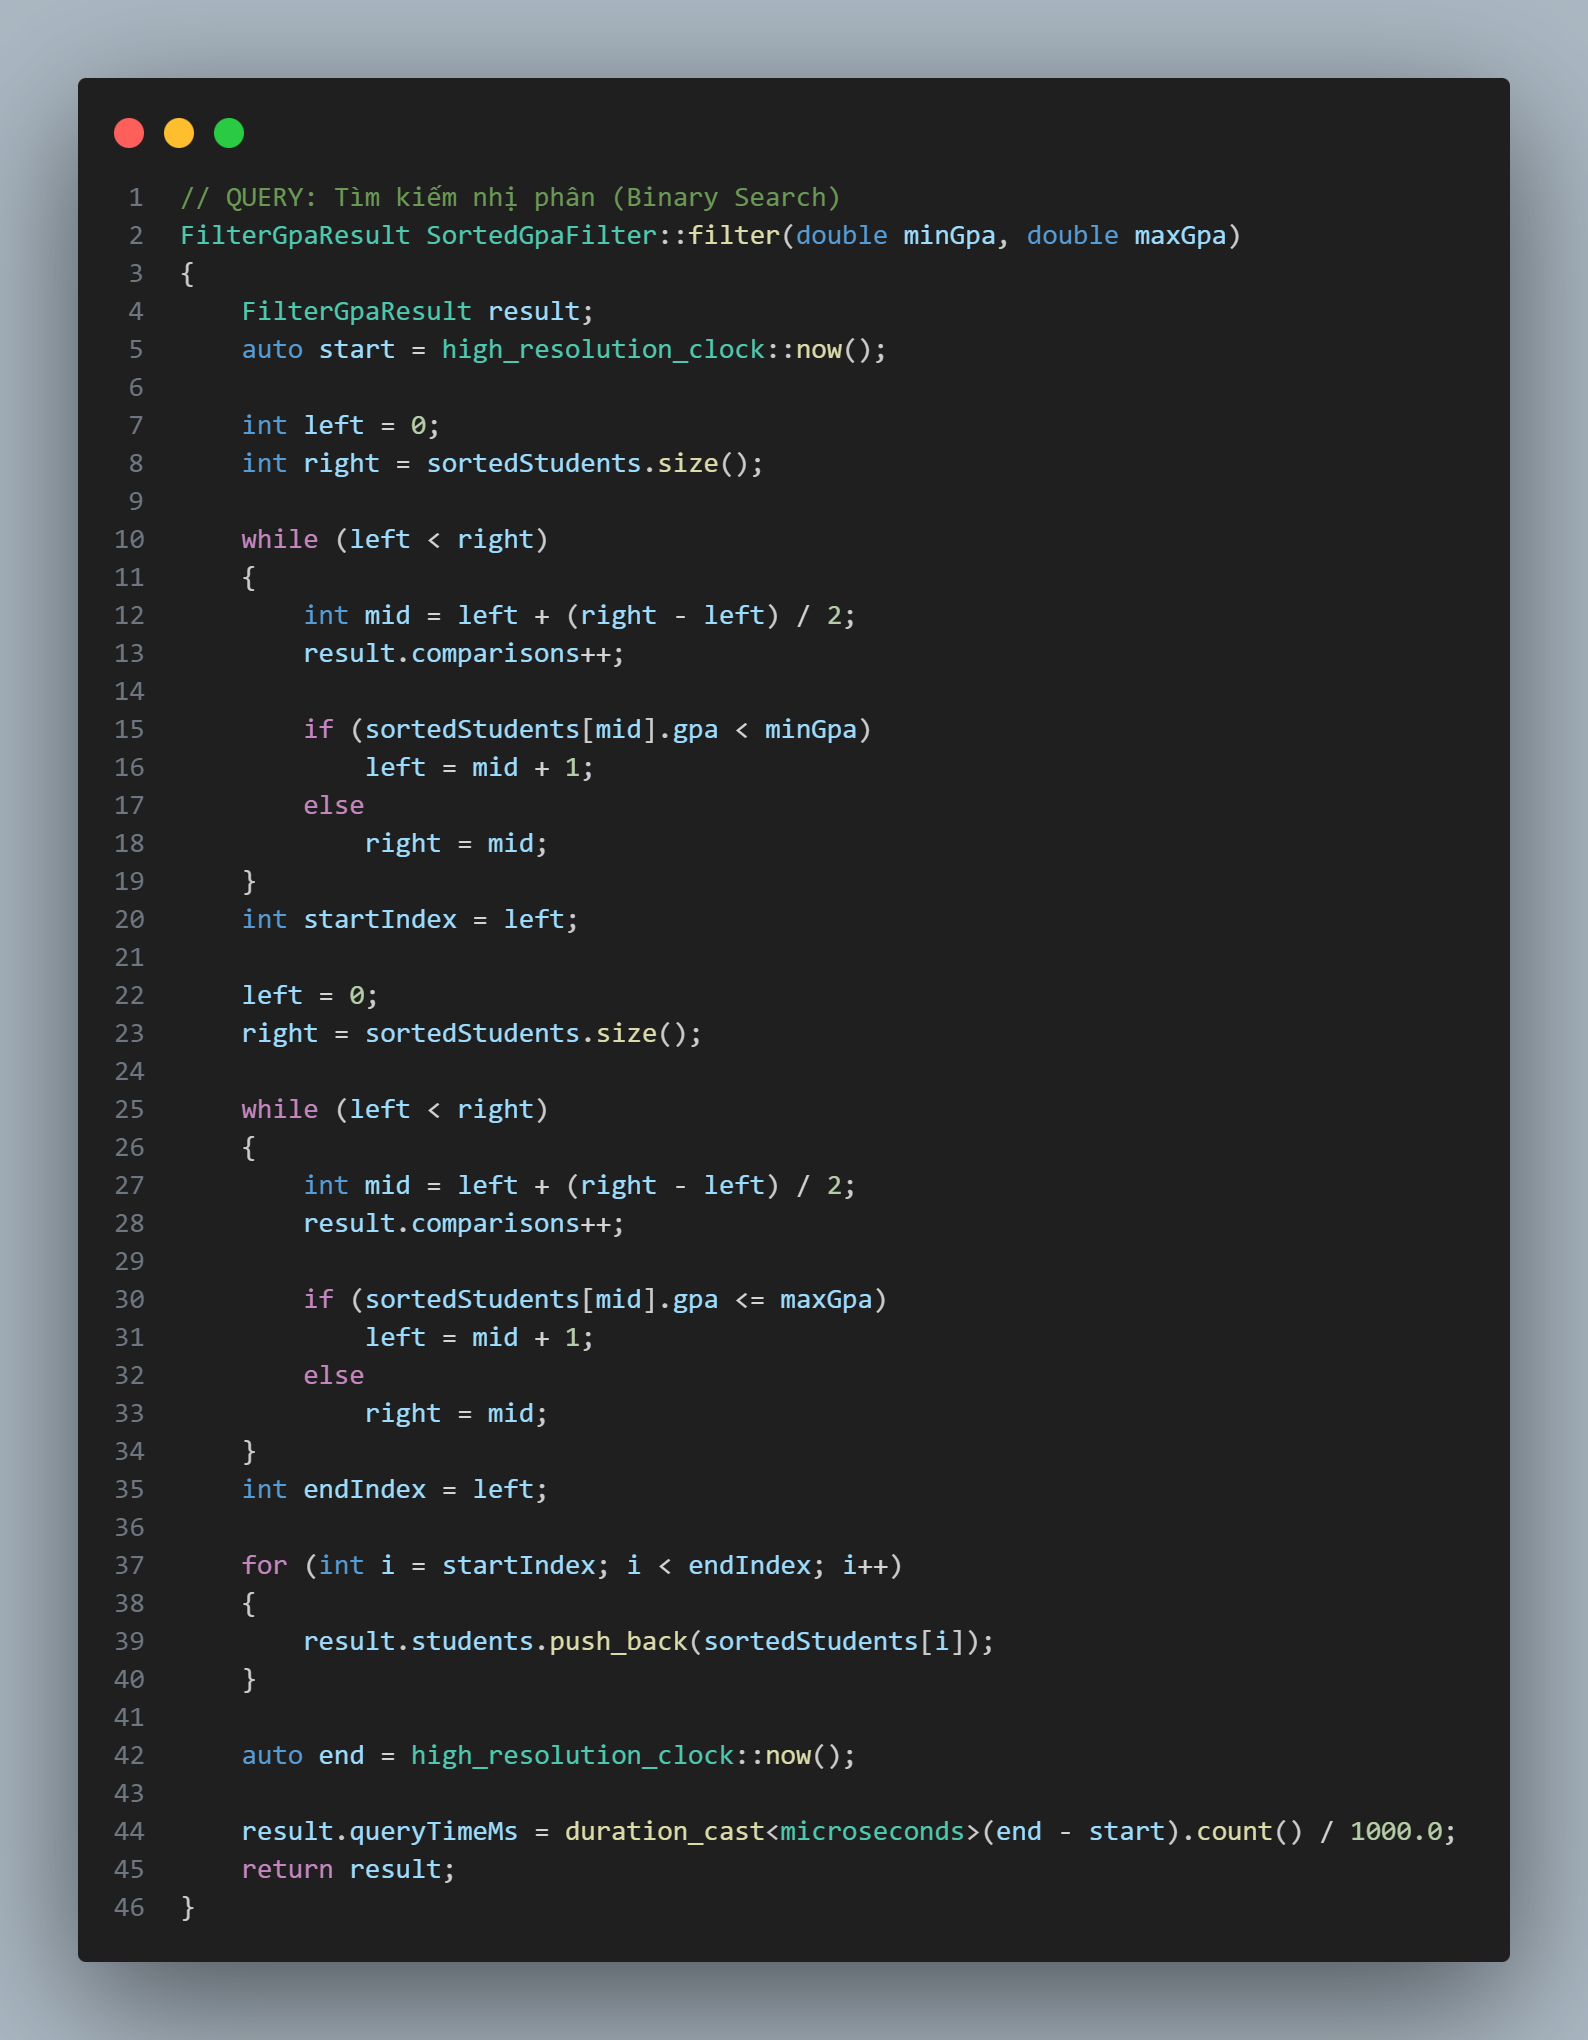
\includegraphics[width=0.52\textwidth]{code_binary_search_range.png}
\caption{Mã nguồn thuật toán Binary Search 2 đầu biên trích xuất khoảng GPA}
\label{fig:code_binary_search_range}
\end{figure}

Tổng thời gian xác định đoạn mảng kết quả là $2 \cdot O(\log N) = O(\log N)$. Sau đó, hệ thống không sao chép $K = \text{endIndex} - \text{startIndex}$ bản ghi sinh viên, mà trả \texttt{GpaRangeViewResult} tham chiếu đến đoạn $[startIndex, endIndex)$. Vì vậy chi phí tạo kết quả là $O(\log N)$; chỉ khi tầng gọi duyệt toàn bộ kết quả để hiển thị hoặc xuất dữ liệu thì mới phát sinh thêm $O(K)$.

Luồng vận hành lọc sinh viên theo khoảng điểm GPA (Yêu cầu RQ2) được thể hiện chi tiết qua Sơ đồ tuần tự trong Hình \ref{fig:seq_rq2_range}: tiếp nhận tham số \texttt{minGPA} và \texttt{maxGPA}, kiểm tra hợp lệ, chạy tìm kiếm nhị phân 2 đầu biên trên mảng \texttt{SortedGpaFilter} để xác định $[startIndex, endIndex)$, trả về range view không sao chép bản ghi và chỉ dereference các phần tử cần hiển thị khi đóng gói JSON preview.

\begin{figure}[htbp]
\centering
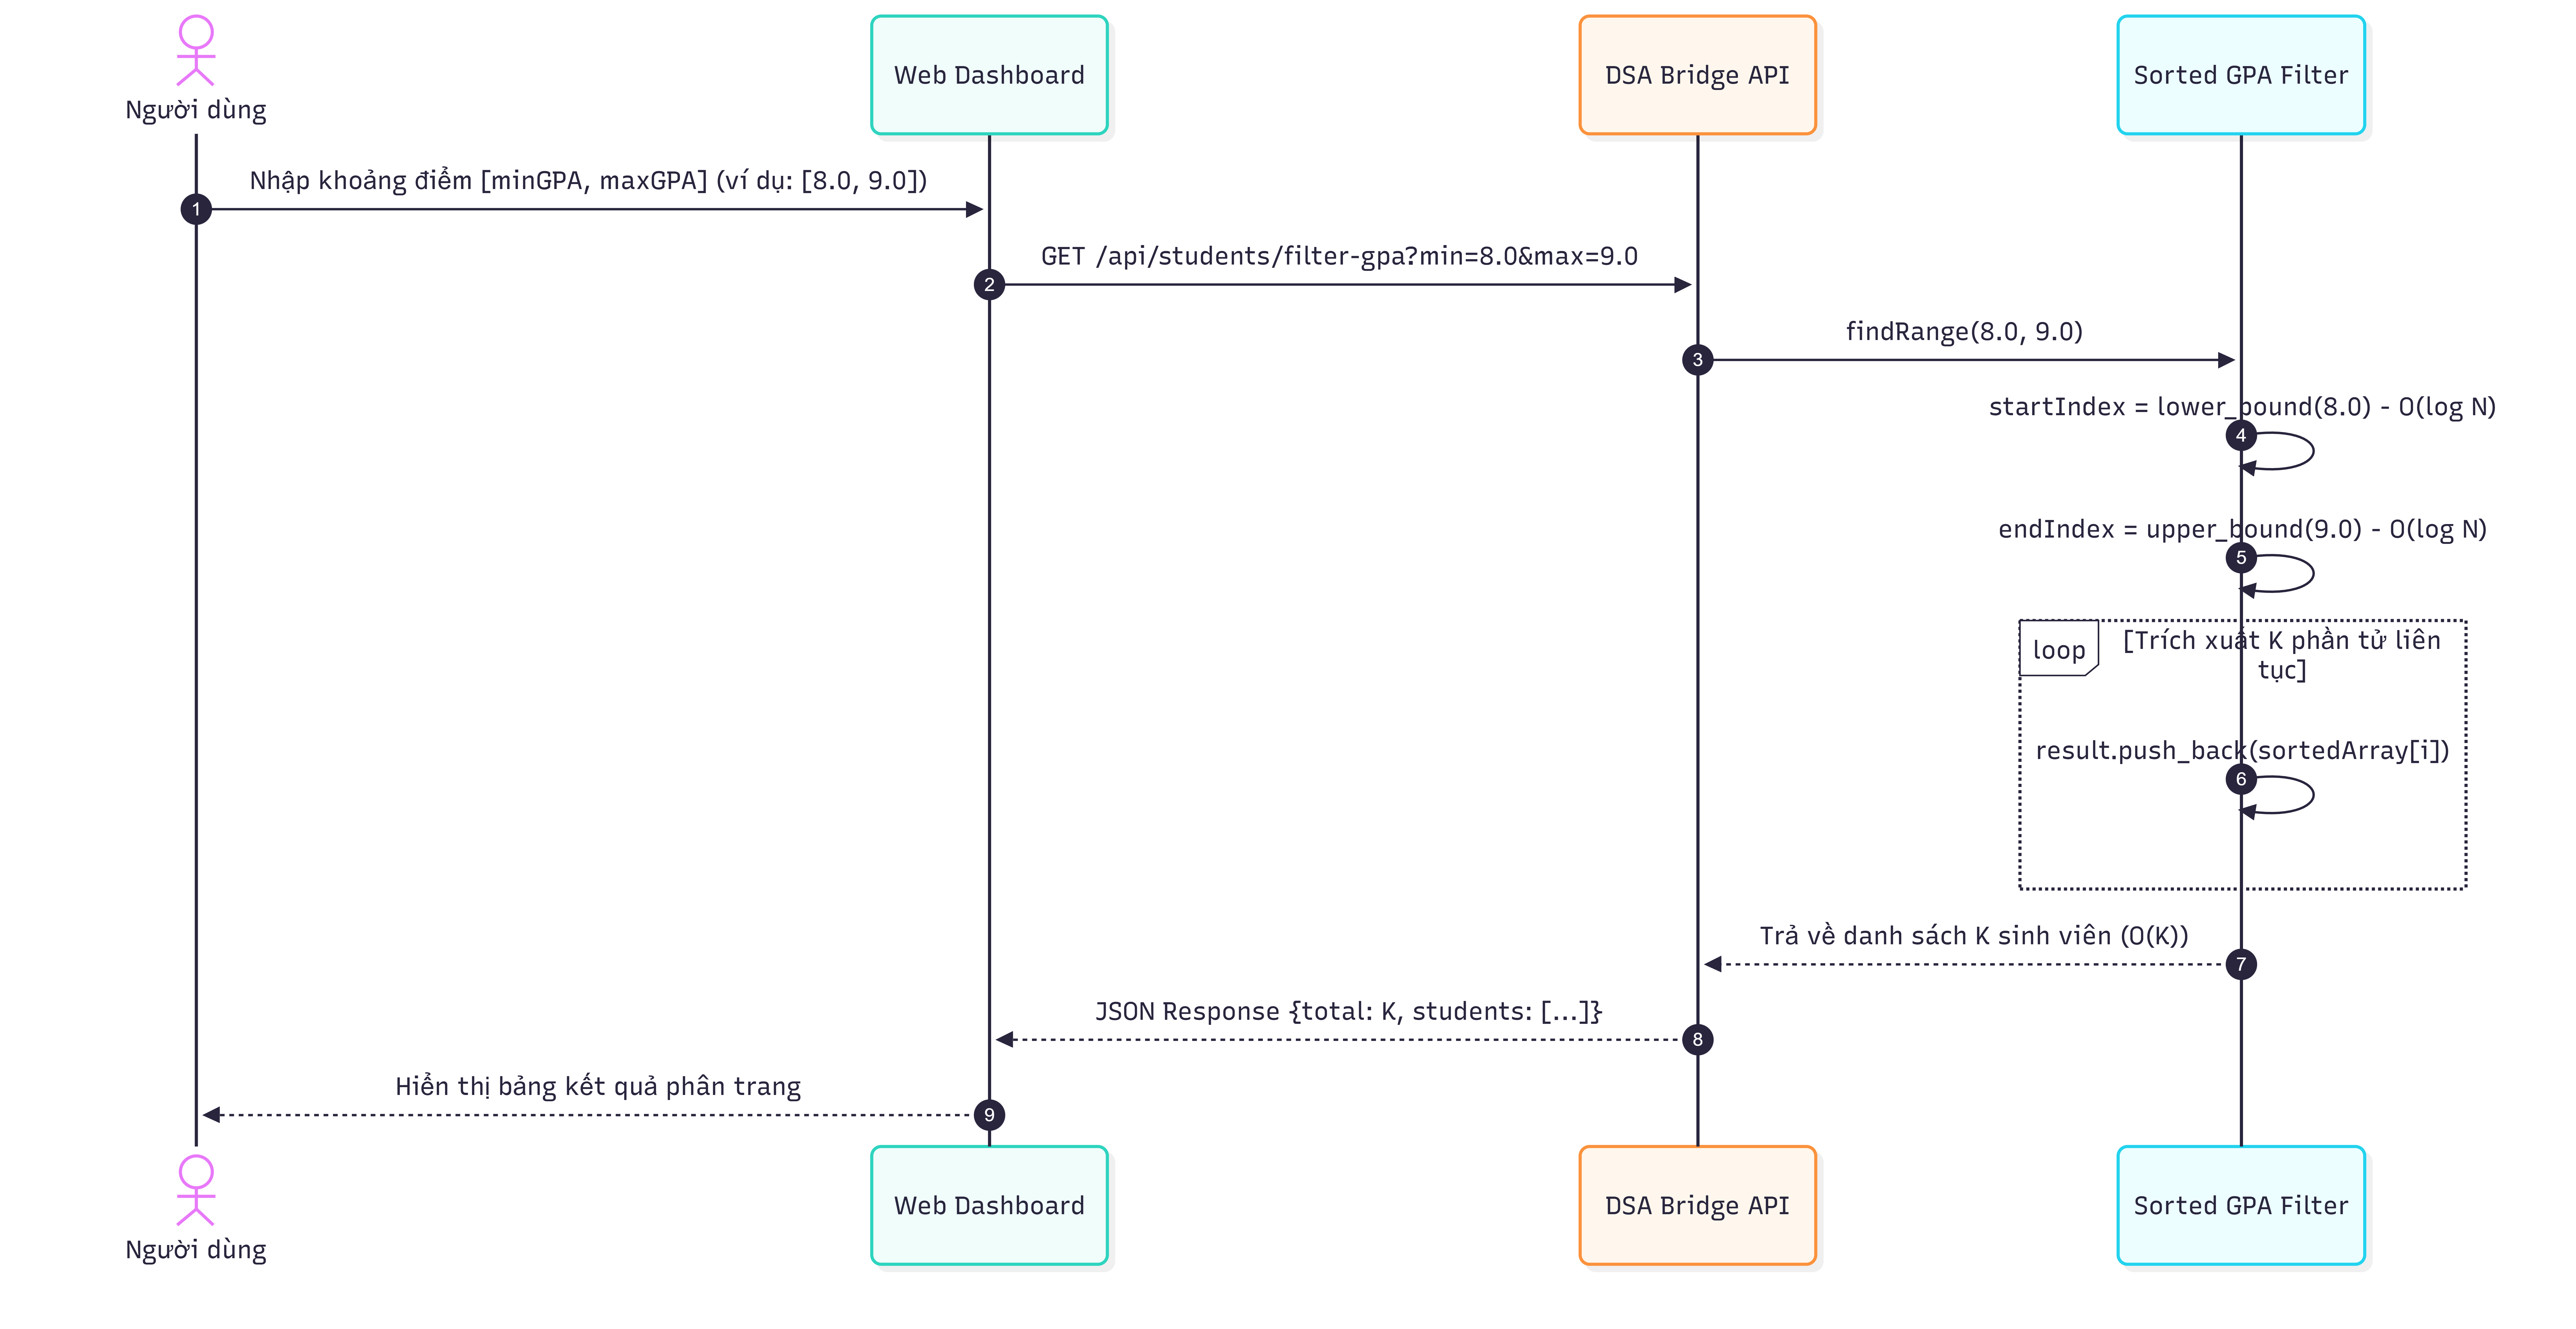
\includegraphics[width=0.72\textwidth]{seq_rq2_range.png}
\caption{Sơ đồ tuần tự (Sequence Diagram) luồng lọc sinh viên theo khoảng GPA}
\label{fig:seq_rq2_range}
\end{figure}

\subsubsection*{2.3.3. Hiện thực bộ lọc theo mã lớp học phần (RQ1) bằng Class Index View}
\addcontentsline{toc}{subsubsection}{2.3.3. Hiện thực bộ lọc theo mã lớp học phần (RQ1) bằng Class Index View}

Đối với yêu cầu lọc danh sách sinh viên theo mã lớp học phần (\texttt{classId}, RQ1), nhóm xây dựng \texttt{ClassIndexFilter} theo hướng Class Index View. Pha \texttt{build()} duyệt một lần qua mảng sinh viên và lưu \texttt{unordered\_map<string, vector<int>>}, trong đó mỗi khóa \texttt{classId} trỏ đến danh sách chỉ số sinh viên thuộc lớp đó. Pha \texttt{filterView()} chỉ thực hiện tra cứu hash trung bình $O(1)$ và trả về con trỏ tới \texttt{vector<int>} đã có sẵn, nên không sao chép $K$ đối tượng \texttt{Student} và cũng không sao chép lại $K$ chỉ số khi chỉ cần benchmark query.

Chi phí xây dựng của cấu trúc này là $O(N)$ thời gian và $O(N)$ bộ nhớ chỉ mục. Sau khi build, mỗi truy vấn theo lớp có chi phí trung bình $O(1)$ để lấy view; chỉ khi tầng giao diện/API cần liệt kê kết quả thì mới phát sinh thêm $O(K)$ để dereference các chỉ số cần hiển thị.
\subsection*{2.4. Hiện thực tầng lưu trữ bền vững và cơ chế nạp dữ liệu hàng loạt}
\addcontentsline{toc}{subsection}{2.4. Hiện thực tầng lưu trữ bền vững và cơ chế nạp dữ liệu hàng loạt}

\subsubsection*{2.4.1. Thiết kế cấu trúc lưu trữ file dữ liệu (JSON / CSV)}
\addcontentsline{toc}{subsubsection}{2.4.1. Thiết kế cấu trúc lưu trữ file dữ liệu (JSON / CSV)}

Dữ liệu thực nghiệm của hệ thống được lưu trữ bền vững trong tệp \texttt{database.json} và \texttt{database.csv} trên đĩa cứng. Mỗi bản ghi bao gồm đầy đủ 4 trường thông tin đã chuẩn hóa: \texttt{id}, \texttt{name}, \texttt{classId} (lớp học phần), và \texttt{gpa} (thang điểm 10). Cấu trúc tệp được định dạng chặt chẽ, tối ưu dung lượng lưu trữ trên đĩa để hỗ trợ việc đọc tuần tự khối lượng lớn (khoảng vài trăm MB đến hơn 1 GB dữ liệu văn bản thô).

\subsubsection*{2.4.2. Cơ chế nạp dữ liệu hàng loạt (Bulk Load) vào bộ nhớ RAM}
\addcontentsline{toc}{subsubsection}{2.4.2. Cơ chế nạp dữ liệu hàng loạt (Bulk Load) vào bộ nhớ RAM}

Khi hệ thống khởi động, tầng Persistence đọc tệp dữ liệu thông qua \texttt{std::ifstream}. Quá trình nạp dữ liệu diễn ra theo quy trình một chiều: Đọc bản ghi $\rightarrow$ Chuẩn hóa dữ liệu $\rightarrow$ Đưa vào vùng nhớ chính \texttt{std::vector<Student>} $\rightarrow$ Xây dựng Bảng băm đóng với con trỏ về dữ liệu gốc $\rightarrow$ Thực hiện Floyd Build Heap trên bản sao \texttt{maxHeap} $\rightarrow$ Sắp xếp mảng con trỏ \texttt{sortedStudents} theo GPA. Cơ chế nạp hàng loạt này giúp các cấu trúc sẵn sàng trước khi chạy benchmark.

\textbf{Ghi chú phạm vi benchmark:} Các phép đo hiệu năng trong báo cáo được thực hiện trên tập dữ liệu đã nạp xong. Phần CRUD trong Web Dashboard phục vụ minh họa quản lý dữ liệu và không được tính vào các kết quả benchmark cốt lõi. Trong code hiện tại, HashTable và SortedGPA lưu con trỏ về vector gốc nên cần được build lại sau khi dữ liệu thay đổi; Heap sử dụng vùng dữ liệu sao chép riêng.

Chu trình nạp dữ liệu hàng loạt và đồng bộ hóa đa cấu trúc chỉ mục (Bulk Loading \& Multi-Index Synchronization Flow) được minh họa chi tiết trong Sơ đồ tuần tự Hình \ref{fig:seq_bulk_load}, bao gồm các bước phối hợp chặt chẽ:

Khởi đầu, tiến trình kích hoạt lệnh nạp tệp thông qua phương thức \texttt{loadFromFile("database.json")} trên lớp điều phối trung tâm \texttt{StudentDatabase}.

Tầng Persistence mở luồng tệp tin với bộ đệm luồng mở rộng (\textit{Stream Buffer}), đọc tuần tự các dòng văn bản, phân tích cú pháp dữ liệu và xác định tổng quy mô $N = 10.000.000$ bản ghi sinh viên.

Tầng DSA Core thực hiện cấp phát trước dung lượng (\texttt{reserve}) cho mảng thực thể chính \texttt{std::vector<Student>}. Bước này giúp loại trừ chi phí cấp phát lại bộ nhớ và giữ cố định địa chỉ các phần tử trước khi các cấu trúc chỉ mục lưu con trỏ trỏ vào.

Hệ thống tiến hành xây dựng Bảng băm đóng (\texttt{HashTable}): mảng băm được cấp phát $M = 2N + 1 = 20.000.001$ ô nhớ. Toàn bộ $N$ con trỏ trỏ về bản ghi gốc được băm bằng FNV-1a và chèn vào bảng theo giải thuật dò tuyến tính để sẵn sàng cho yêu cầu tra cứu MC1.

Đồng thời, ba cấu trúc chỉ mục còn lại được khởi tạo đồng bộ: Max-Heap nạp dữ liệu và vun đống Floyd từ dưới lên với chi phí $O(N)$; mảng con trỏ GPA được sắp xếp bằng \texttt{std::sort} ($O(N \log N)$) để phục vụ RQ2; và ClassIndex duyệt qua mảng một lần để gom nhóm chỉ số theo lớp vào \texttt{unordered\_map<string, vector<int>>} phục vụ RQ1.

Khi toàn bộ 4 cấu trúc trong RAM đã hoàn tất việc khởi tạo, hệ thống phát tín hiệu sẵn sàng (Engine Ready) và chuyển sang trạng thái phục vụ các truy vấn tức thời từ người dùng.

\begin{figure}[htbp]
\centering
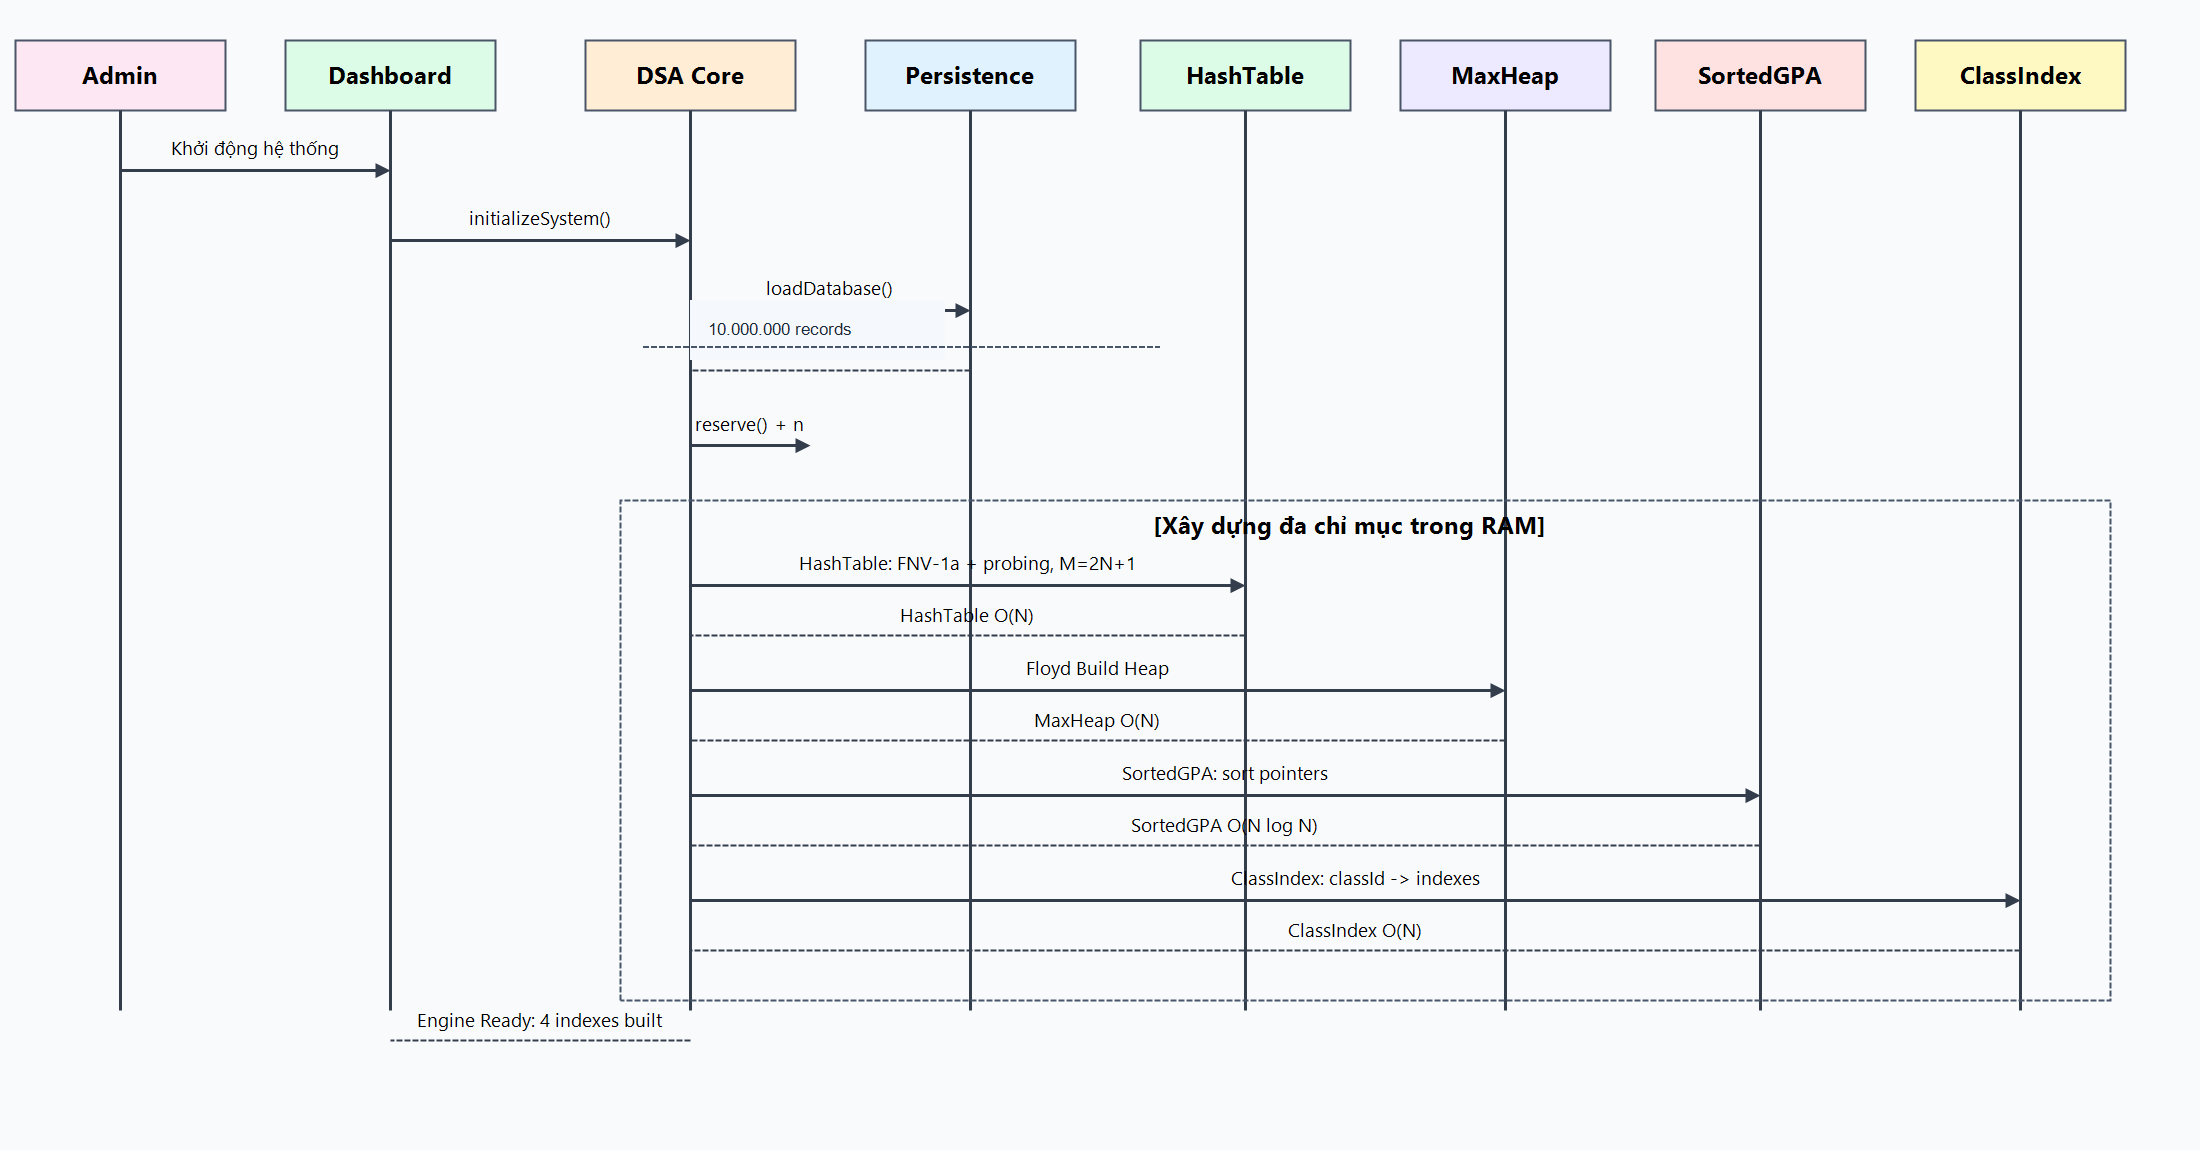
\includegraphics[width=0.76\textwidth]{seq_bulk_load.png}
\caption{Sơ đồ tuần tự (Sequence Diagram) luồng khởi tạo và nạp dữ liệu hàng loạt (Bulk Load)}
\label{fig:seq_bulk_load}
\end{figure}

\subsubsection*{2.4.3. Đảm bảo nguyên tắc độc lập giữa lưu trữ và xử lý truy vấn}
\addcontentsline{toc}{subsubsection}{2.4.3. Đảm bảo nguyên tắc độc lập giữa lưu trữ và xử lý truy vấn}

Nhóm tuân thủ nguyên tắc kiến trúc: Tệp tin lưu trữ chỉ được truy cập một lần duy nhất lúc khởi động để nạp dữ liệu thô vào RAM. Mọi thao tác tìm kiếm MC1, MC2, lọc RQ1, RQ2 đều được xử lý trên cấu trúc dữ liệu trong bộ nhớ (In-memory DSA Core). Hệ thống không thực hiện đọc lại tệp hay sử dụng các cơ chế truy vấn của cơ sở dữ liệu để giải quyết bài toán.

\subsection*{2.5. Xây dựng giao diện tương tác và trực quan hóa dữ liệu}
\addcontentsline{toc}{subsection}{2.5. Xây dựng giao diện tương tác và trực quan hóa dữ liệu}

\subsubsection*{2.5.1. Thiết kế giao diện dòng lệnh CLI tương tác nhanh}
\addcontentsline{toc}{subsubsection}{2.5.1. Thiết kế giao diện dòng lệnh CLI tương tác nhanh}

Hệ thống cung cấp một module giao diện dòng lệnh (CLI Engine) bằng C++ hỗ trợ các lệnh tương tác tức thời: tra cứu theo MSSV, lấy GPA cao nhất, lọc theo lớp, lọc theo khoảng điểm và kích hoạt chế độ Benchmark tự động. Giao diện CLI cho phép các kỹ sư kiểm thử nhanh chóng tính đúng đắn và đo thời gian thực thi bằng \texttt{std::}\allowbreak\texttt{chrono::}\allowbreak\texttt{high\_}\allowbreak\texttt{resolution\_clock} với độ chính xác cao.

\subsubsection*{2.5.2. Xây dựng module trực quan hóa cấu trúc dữ liệu và benchmark}
\addcontentsline{toc}{subsubsection}{2.5.2. Xây dựng module trực quan hóa cấu trúc dữ liệu và benchmark}

Để nâng cao tính trực quan và phục vụ đánh giá năng lực, nhóm xây dựng Web Dashboard hiện đại bằng Next.js và React kết hợp Ant Design. Giao diện Web giao tiếp với C++ Engine qua API Bridge, hiển thị chi tiết các bảng dữ liệu, trạng thái các ô nhớ trong bảng băm, cây Max-Heap, và trực quan hóa các biểu đồ đối sánh thời gian thực thi Benchmark bằng biểu đồ cột so sánh trực tiếp với Baseline.

\subsection*{2.6. Thiết kế kịch bản kiểm thử tự động và xử lý trường hợp biên}
\addcontentsline{toc}{subsection}{2.6. Thiết kế kịch bản kiểm thử tự động và xử lý trường hợp biên}

\subsubsection*{2.6.1. Xây dựng bộ Unit Test tự động cho các cấu trúc tự cài đặt}
\addcontentsline{toc}{subsubsection}{2.6.1. Xây dựng bộ Unit Test tự động cho các cấu trúc tự cài đặt}

Nhóm đã xây dựng bộ kiểm thử tự động toàn diện bao quát các phương thức và thao tác cốt lõi của Bảng băm đóng và Max-Heap. Mỗi cấu trúc dữ liệu đều trải qua các bài kiểm thử tính đúng đắn về khởi tạo chỉ mục, tra cứu thành công, tra cứu khóa không tồn tại, kiểm soát xung đột chỉ số, vun đống Floyd từ dưới lên và duy trì bất biến cấu trúc Max-Heap sau các kịch bản kiểm thử.

\subsubsection*{2.6.2. Kiểm thử xử lý dữ liệu trùng lặp, dữ liệu rỗng và tràn ngưỡng}
\addcontentsline{toc}{subsubsection}{2.6.2. Kiểm thử xử lý dữ liệu trùng lặp, dữ liệu rỗng và tràn ngưỡng}

Hệ thống được kiểm thử kỹ lưỡng trên 5 kịch bản trường hợp biên (Edge Cases) tiêu biểu:

\textbf{Tập dữ liệu rỗng ($N = 0$):} Hệ thống phản hồi an toàn với thông báo hợp lệ, không phát sinh lỗi truy cập vùng nhớ con trỏ null.

\textbf{Tra cứu mã số không tồn tại:} Bảng băm kết thúc vòng dò ngay khi gặp ô trống đầu tiên và trả về \texttt{nullptr} trong thời gian $O(1)$ mà không gặp hiện tượng treo chương trình.

\textbf{Xử lý khóa chính trùng lặp:} Cơ chế phát hiện trùng mã sinh viên được đặt tại tầng CRUD/Persistence khi thêm mới hồ sơ thông qua hàm \texttt{findIndexById} trước khi lưu vào tệp dữ liệu.

\textbf{Nhiều sinh viên cùng đạt GPA tối đa ($10.0$):} Max-Heap tự động kích hoạt toán tử phân định đồng hạng (Tie-break), ưu tiên sinh viên có MSSV nhỏ hơn theo thứ tự từ điển nằm tại nút gốc.

\textbf{Khoảng điểm truy vấn không hợp lệ:} Với các tham số như $\text{minGPA} > \text{maxGPA}$ hoặc điểm nằm ngoài dải $[0.0, 10.0]$, hệ thống tự động nhận diện và gửi cảnh báo từ chối truy vấn rõ ràng.

\subsubsection*{2.6.3. Kiểm thử tính ổn định khi chạy tải truy vấn liên tục}
\addcontentsline{toc}{subsubsection}{2.6.3. Kiểm thử tính ổn định khi chạy tải truy vấn liên tục}

Nhóm thực hiện bài kiểm thử sức chịu tải (Stress Test) với các workload truy vấn lặp trên tập dữ liệu hiện tại $10.000.000$ bản ghi. Kết quả ghi nhận hệ thống vận hành ổn định, không quan sát thấy dấu hiệu rò rỉ bộ nhớ (Memory Leak) hay suy giảm tốc độ xử lý trong quá trình kiểm thử.

\subsection*{2.7. Thực nghiệm đo đạc Benchmark hiệu năng trên tập dữ liệu quy mô lớn}
\addcontentsline{toc}{subsection}{2.7. Thực nghiệm đo đạc Benchmark hiệu năng trên tập dữ liệu quy mô lớn}

\subsubsection*{2.7.1. Môi trường phần cứng, hệ điều hành và phương pháp luận đo lường}
\addcontentsline{toc}{subsubsection}{2.7.1. Môi trường phần cứng, hệ điều hành và phương pháp luận đo lường}

Toàn bộ các phép đo đạc Benchmark đối sánh được thực hiện trên cùng một môi trường phần cứng và cấu hình phần mềm đồng nhất:

\textbf{Vi xử lý (CPU):} Intel Core i7-13620H (10 Cores, 16 Threads), bộ nhớ đệm Cache 24MB.

\textbf{Bộ nhớ RAM:} 16 GB DDR4 Bus 3200 MHz.

\textbf{Hệ điều hành:} Microsoft Windows 11 64-bit.

\textbf{Trình biên dịch:} GCC / MinGW-w64 hỗ trợ chuẩn C++20, cờ tối ưu hóa \texttt{-O3}.

\textbf{Công cụ đo thời gian:} Sử dụng đồng hồ độ phân giải cao của thư viện chuẩn C++ (\texttt{std::chrono::high\_resolution\_clock}).

\textbf{Phương pháp luận đo lường (Benchmark Methodology):} Để giảm nhiễu hệ điều hành và tránh nhầm lẫn giữa chi phí thuật toán với chi phí giao diện, nhóm tách hai loại số liệu. Bảng số trong báo cáo là microbenchmark C++ Core: thực hiện batch workload trực tiếp trong C++, gán kết quả vào biến lưu trữ để tránh Dead Code Elimination khi bật \texttt{-O3}. Harness đo được biên dịch riêng bằng lệnh \texttt{g++ -std=c++20 -O3}. Các hình Dashboard ở cuối phần này minh họa giao diện và luồng API, có thêm chi phí JSON/IPC/render nên không được dùng để thay thế số microbenchmark. Với RQ1 và RQ2, số liệu Final Solution đo chi phí định vị chỉ mục và tạo view; chi phí materialize hoặc serialize toàn bộ $K$ kết quả được tách khỏi pha query lõi. Các số RQ1/RQ2 thể hiện chi phí của hai thiết kế API hoàn chỉnh hiện tại: baseline materialize kết quả còn final trả view, vì vậy mức chênh lệch không được diễn giải hoàn toàn là hệ quả của riêng độ phức tạp tìm kiếm. Do thời gian một truy vấn RQ1/RQ2 ở nhánh final nằm trên thang nano-giây trong môi trường hot-cache, giá trị tuyệt đối chỉ dùng để thể hiện xu hướng; phần đánh giá chính dựa trên số phép toán, số phần tử phải quét và độ phức tạp tiệm cận.

\textbf{Cấu hình workload thực nghiệm:} Tập dữ liệu ban đầu nạp từ \texttt{data/database.json}, sau đó dùng cơ chế bulk-add trong RAM để đạt đúng $10.000.000$ sinh viên. Harness chạy $5$ lượt warm-up và $9$ mẫu đo chính, lấy median làm số đại diện. MC1 chạy $1.000$ truy vấn MSSV cố định, gồm $950$ khóa tồn tại và $50$ khóa không tồn tại. MC2 chạy $100$ lần gọi truy xuất GPA cao nhất. RQ1 lọc lớp dày nhất được chọn tự động trong tập dữ liệu sinh ra (\texttt{25KTP02}). RQ2 lọc khoảng GPA $[8.0, 10.0]$. Thời gian nạp/generate dữ liệu 10M trong lần chạy chính là khoảng $2.780$ giây ($2{,}780.468$ ms) và không được tính vào thời gian query của từng cấu trúc.

\begin{table}[H]
\centering
\begingroup
\begin{singlespace}
\setlength{\tabcolsep}{2pt}
\renewcommand{\arraystretch}{1.3}
\begin{tabularx}{\textwidth}{|>{\raggedright\arraybackslash}m{2.3cm}|>{\centering\arraybackslash}m{2.0cm}|>{\centering\arraybackslash}m{2.0cm}|>{\centering\arraybackslash}m{2.0cm}|>{\centering\arraybackslash}m{2.0cm}|>{\raggedright\arraybackslash}X|}
\hline
\textbf{Build structure} & \textbf{Min} & \textbf{Median} & \textbf{Mean} & \textbf{Max} & \textbf{Ghi chú} \\ \hline
HashTable & $389.706$ & $399.537$ & $417.367$ & $523.682$ & $4.902.031$ collision khi build \\ \hline
MaxHeap & $1059.895$ & $1082.449$ & $1094.427$ & $1164.259$ & Floyd Build Heap trên bản sao \texttt{maxHeap} \\ \hline
SortedGPA & $3867.451$ & $4188.674$ & $4201.689$ & $4616.481$ & Tạo mảng con trỏ và \texttt{std::sort} theo GPA \\ \hline
ClassIndex & $215.801$ & $228.897$ & $230.575$ & $252.661$ & Xây dựng \texttt{classId -> indexes} cho RQ1 \\ \hline
\end{tabularx}
\end{singlespace}
\endgroup
\caption{Thời gian build cấu trúc C++ Core trên $10.000.000$ sinh viên (ms)}
\label{tab:core_build_benchmark}
\end{table}

\begin{table}[H]
\centering
\begingroup
\begin{singlespace}
\setlength{\tabcolsep}{3pt}
\renewcommand{\arraystretch}{1.3}
\begin{tabularx}{\textwidth}{|>{\raggedright\arraybackslash}m{2.8cm}|>{\centering\arraybackslash}m{1.9cm}|>{\centering\arraybackslash}m{1.9cm}|>{\centering\arraybackslash}m{1.9cm}|>{\centering\arraybackslash}m{1.9cm}|>{\raggedright\arraybackslash}X|}
\hline
\textbf{Query workload} & \textbf{Min} & \textbf{Median} & \textbf{Mean} & \textbf{Max} & \textbf{Ghi chú} \\ \hline
MC1 Linear Search & $26013.78$ & $26424.51$ & $26543.86$ & $27105.64$ & $1000q$; $5.228$B cmp \\ \hline
MC1 Hash Search & $0.024$ & $0.024$ & $0.025$ & $0.027$ & $1000q$; $1564$ probe \\ \hline
MC2 Linear Max & $3562.16$ & $3819.02$ & $3810.21$ & $4080.99$ & $100$ calls; $1.000$B cmp \\ \hline
MC2 Heap Max & $0.016$ & $0.016$ & $0.016$ & $0.016$ & $100$ heap peek \\ \hline
RQ1 Linear Class & $75.336$ & $77.904$ & $77.730$ & $81.113$ & \texttt{25KTP02}; $K=52.649$ \\ \hline
RQ1 ClassIndex View & $<0.0001$ & $<0.0001$ & $0.00002$ & $0.0001$ & $K=52.649$; $1$ lookup \\ \hline
RQ2 Linear GPA & $313.459$ & $331.479$ & $335.239$ & $361.944$ & $[8,10]$; $K=3.343.566$ \\ \hline
RQ2 Sorted GPA & $0.0001$ & $0.0001$ & $0.00033$ & $0.0012$ & $46$ cmp; range view \\ \hline
\end{tabularx}
\end{singlespace}
\endgroup
\caption{Thời gian query C++ Core trên $10.000.000$ sinh viên, $5$ warm-up và $9$ mẫu đo (ms)}
\label{tab:core_microbenchmark}
\end{table}

\subsubsection*{2.7.2. Kết quả đo thời gian tra cứu MC1 qua các mốc dữ liệu lớn}
\addcontentsline{toc}{subsubsection}{2.7.2. Kết quả đo thời gian tra cứu MC1 qua các mốc dữ liệu lớn}

Nhóm tiến hành đo đạc MC1 bằng workload truy vấn cố định trên tập hiện tại ($25150001$ đến $35150000$). Workload gồm khóa tồn tại rải đều trong dải dữ liệu và một nhóm khóa không tồn tại để kiểm tra điều kiện dừng khi gặp ô trống trong bảng băm. Các ảnh dưới đây minh họa giao diện Dashboard theo từng vị trí khóa; bảng \ref{tab:core_microbenchmark} mới là số liệu C++ Core dùng để kết luận hiệu năng.

\begin{figure}[htbp]
\centering
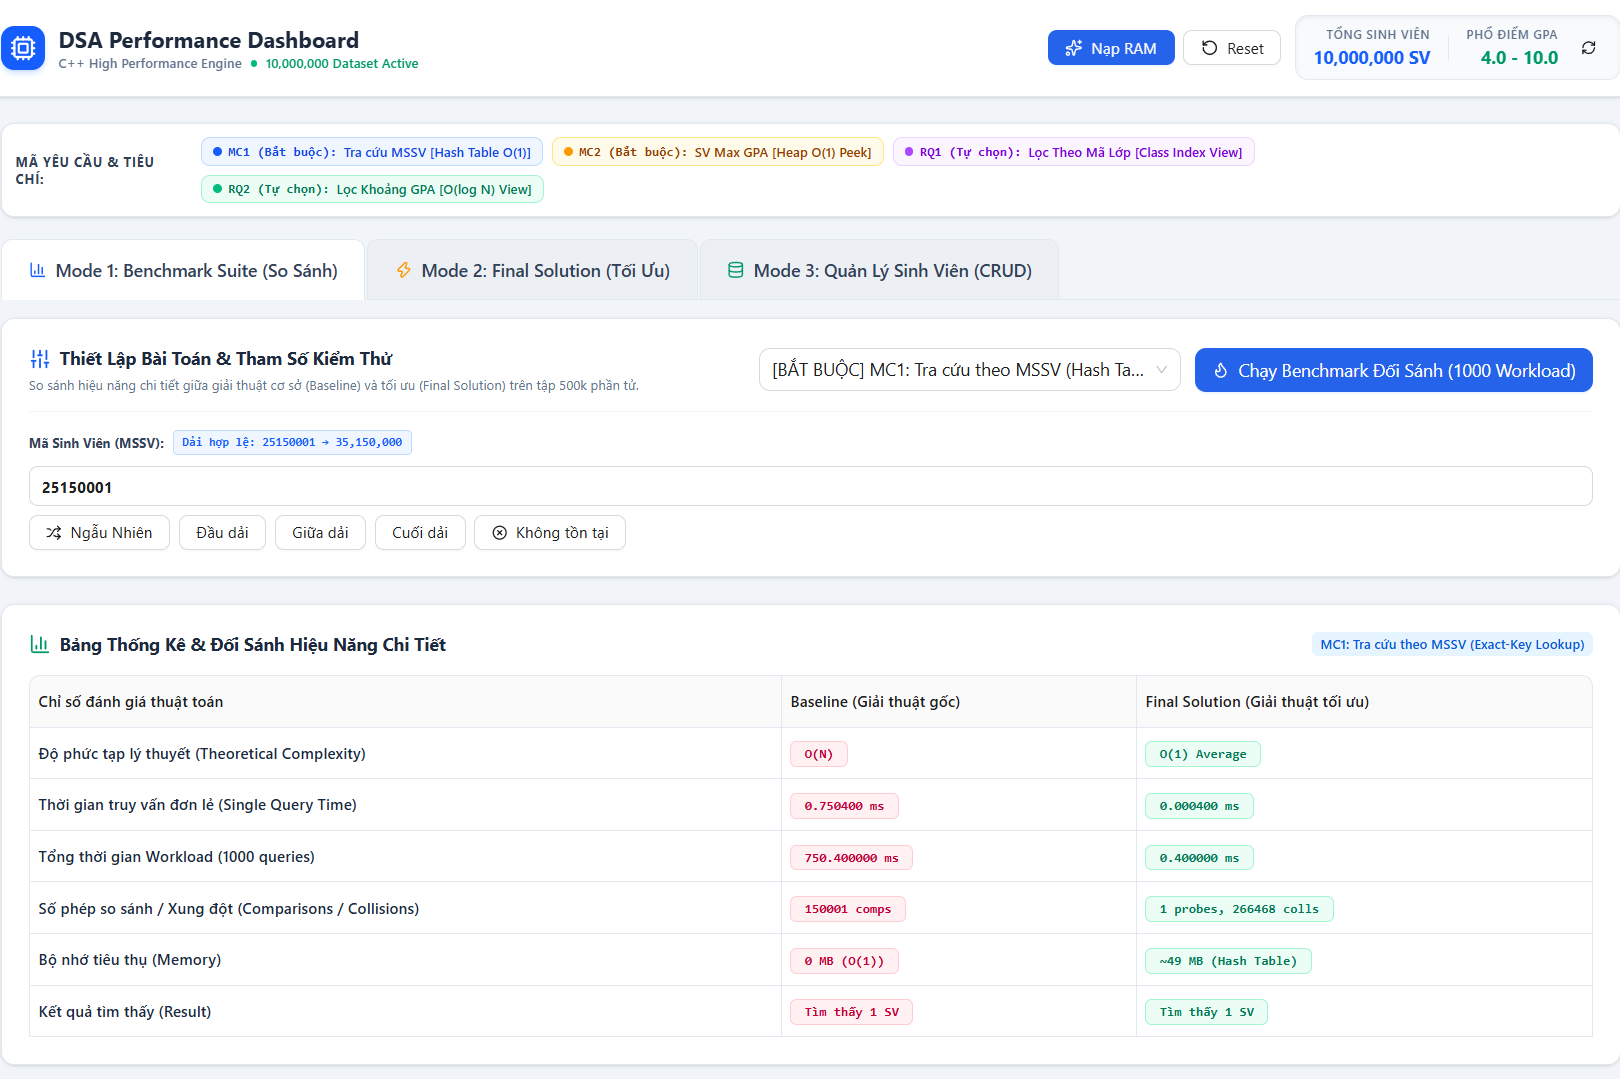
\includegraphics[width=0.56\textwidth]{mc1_dau_dai.png}
\caption{Benchmark MC1 tra cứu MSSV tại đầu dải dữ liệu}
\label{fig:mc1_dau_dai}
\end{figure}

\begin{figure}[htbp]
\centering
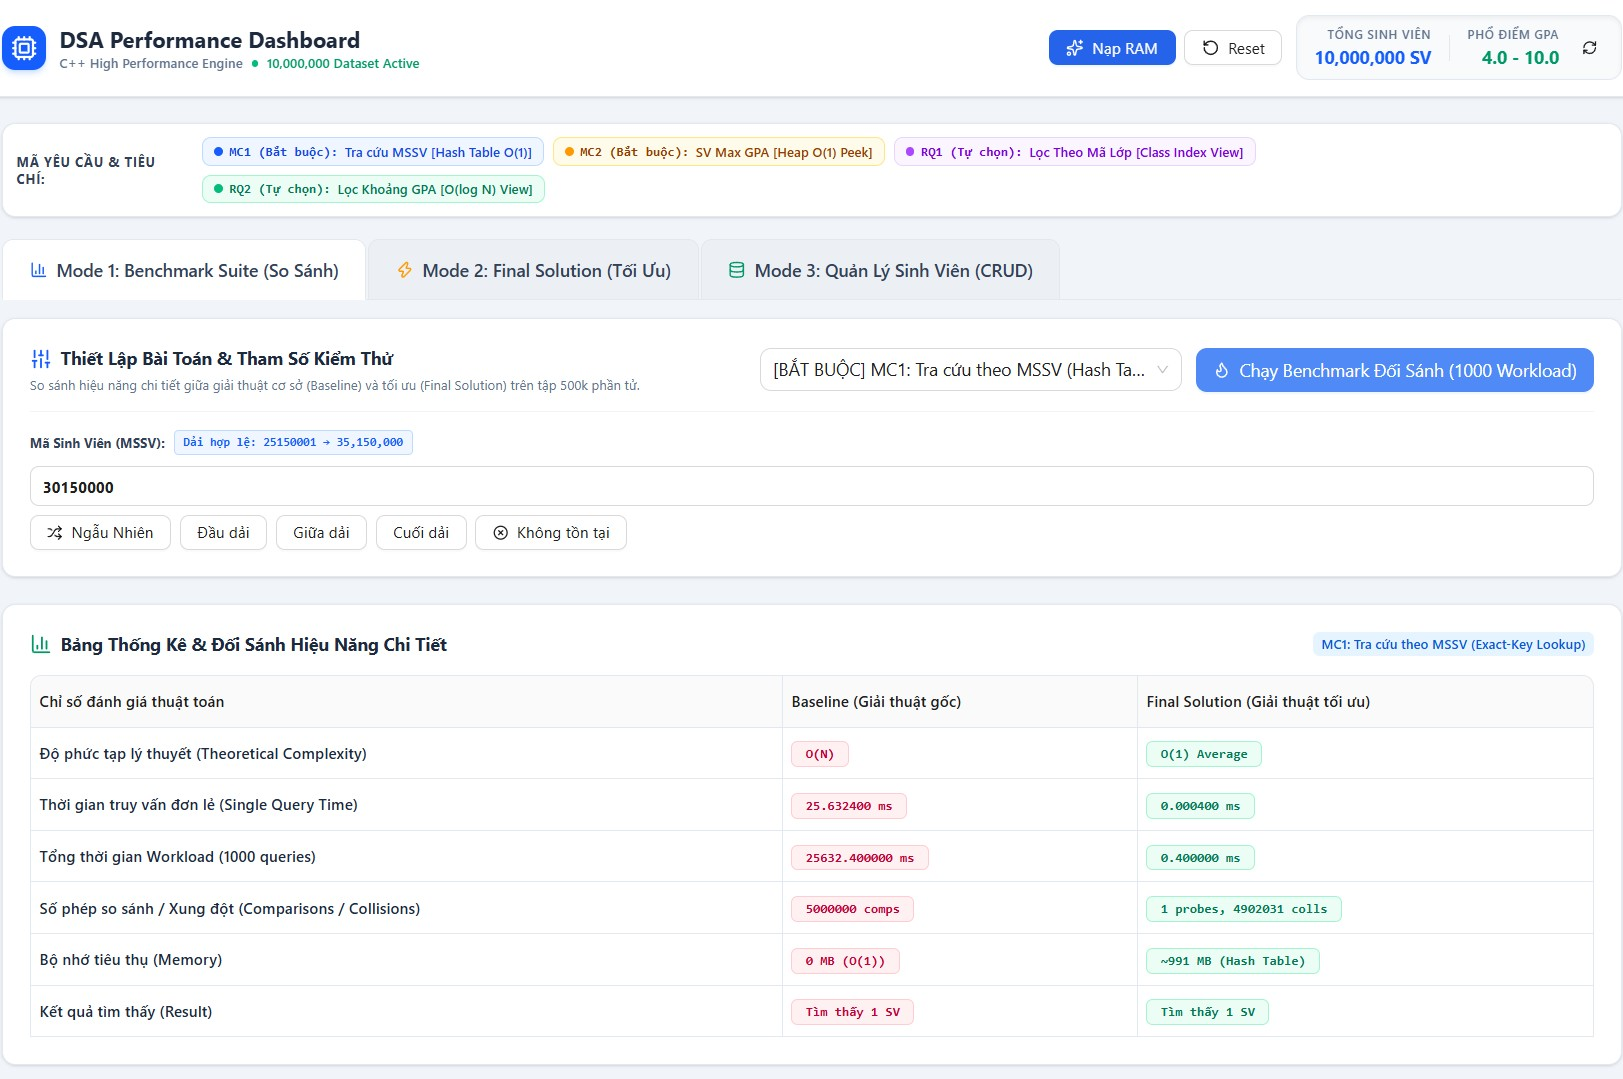
\includegraphics[width=0.56\textwidth]{mc1_giua_dai.jpeg}
\caption{Benchmark MC1 tra cứu MSSV tại giữa dải dữ liệu}
\label{fig:mc1_giua_dai}
\end{figure}

Kết quả thực nghiệm cho thấy Bảng băm đóng duy trì thời gian trả kết quả ở mức rất nhỏ và gần như không phụ thuộc vị trí khóa, trong khi thuật toán duyệt tuyến tính tăng rõ rệt khi khóa nằm sâu trong vector hoặc không tồn tại. Trên workload $1.000$ truy vấn ở tập $10.000.000$ sinh viên, median của Linear Search là $26424.507$ ms, còn Hash Search là $0.024$ ms. Do thao tác Hash lookup quá ngắn, các con số dưới micro-giây cho một truy vấn đơn lẻ chỉ nên được hiểu như xu hướng trung bình sau lặp batch, không phải độ trễ cảm nhận của giao diện.

\begin{figure}[htbp]
\centering
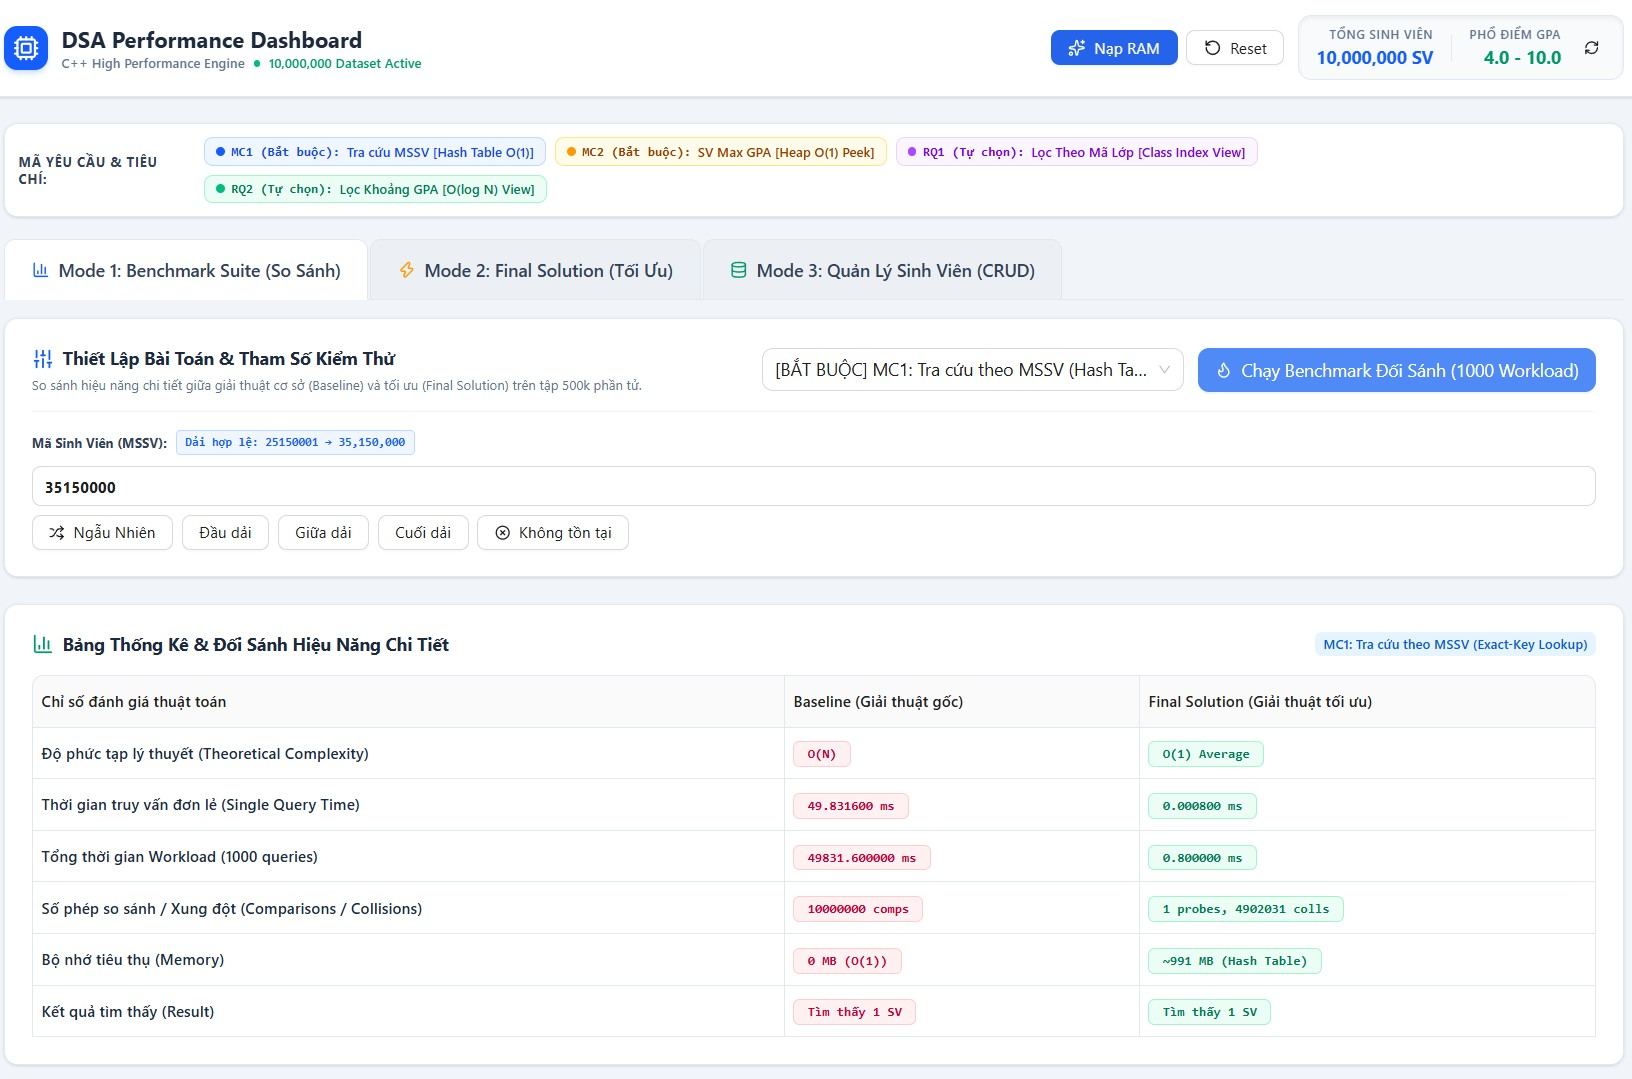
\includegraphics[width=0.56\textwidth]{mc1_cuoi_dai.jpeg}
\caption{Benchmark MC1 tra cứu MSSV tại cuối dải dữ liệu}
\label{fig:mc1_cuoi_dai}
\end{figure}

\begin{figure}[htbp]
\centering
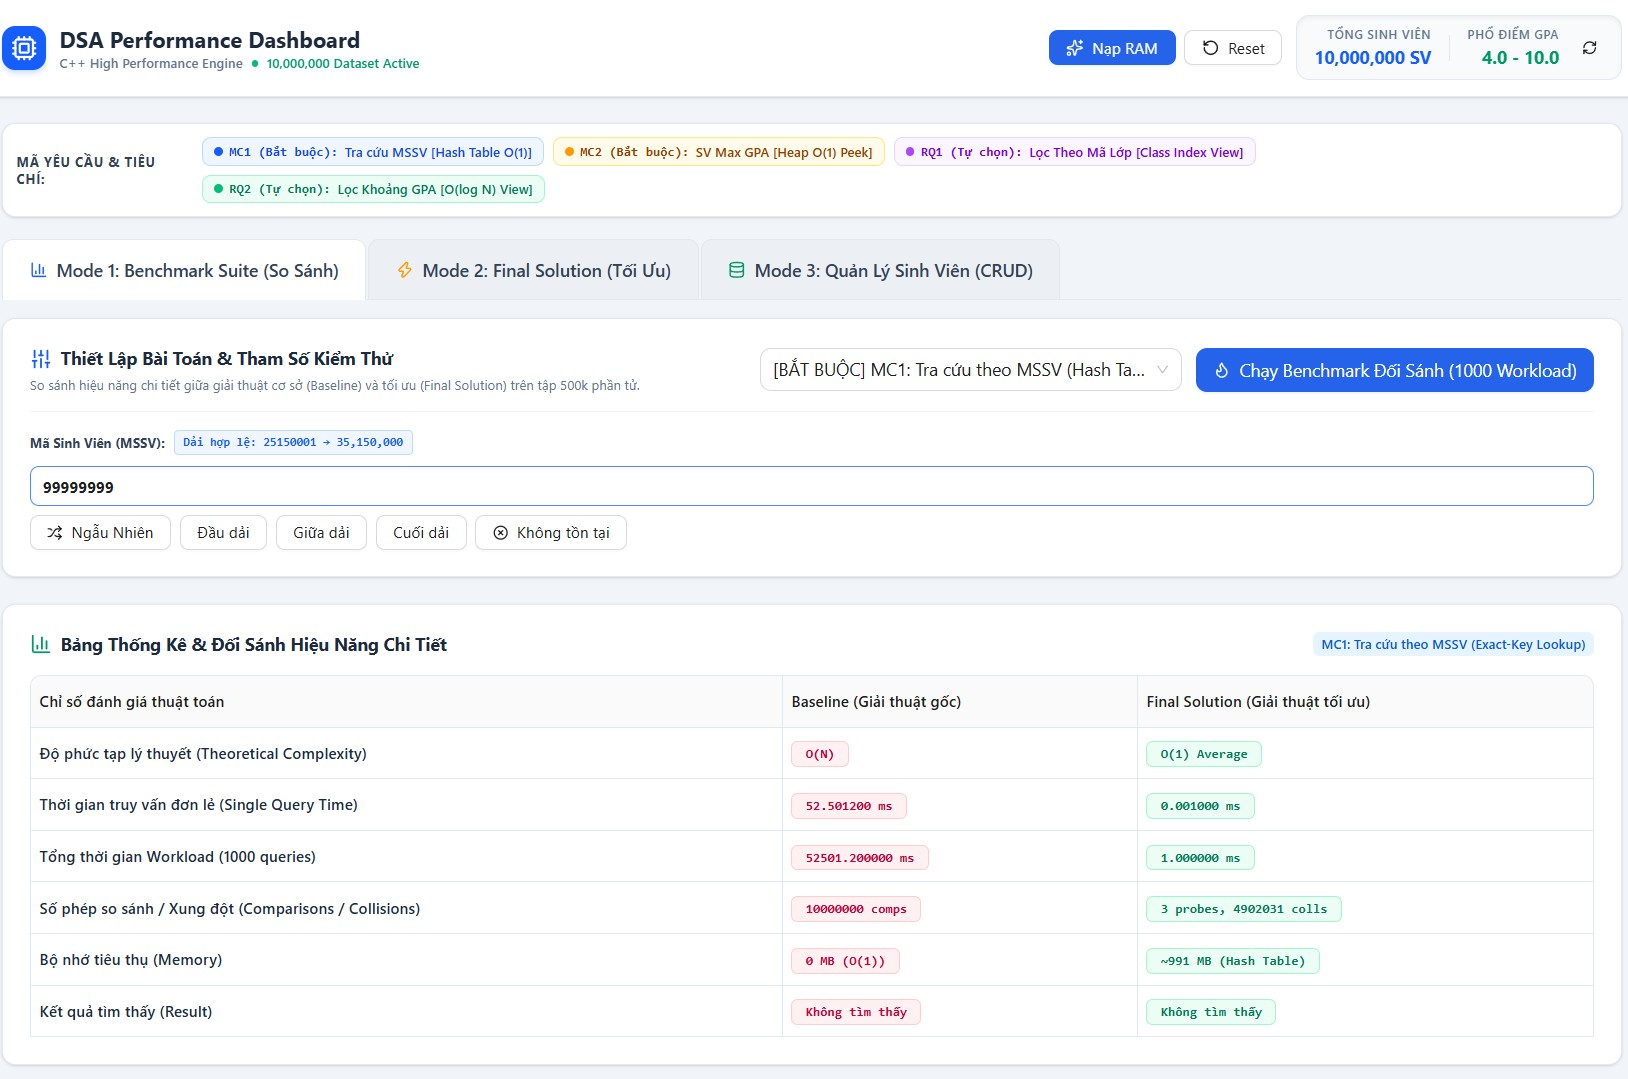
\includegraphics[width=0.56\textwidth]{mc1_khong_ton_tai.jpeg}
\caption{Benchmark MC1 tra cứu MSSV khi khóa không tồn tại trong hệ thống}
\label{fig:mc1_khong_ton_tai}
\end{figure}

\subsubsection*{2.7.3. Kết quả đo thời gian trích xuất cực trị MC2 và xây dựng đống}
\addcontentsline{toc}{subsubsection}{2.7.3. Kết quả đo thời gian trích xuất cực trị MC2 và xây dựng đống}

Đối với yêu cầu MC2, sau khi \texttt{CustomMaxHeapGpaFinder} đã xây dựng xong heap, thao tác trả sinh viên GPA cao nhất chỉ là đọc \texttt{maxHeap[0]}, nên chi phí lý thuyết là $O(1)$. Phần đo thực nghiệm được trình bày theo hướng đối sánh: quét tuyến tính phụ thuộc $N$, còn heap peek gần như hằng số sau khi đã trả chi phí build $O(N)$. Trên $100$ lần gọi ở tập $10.000.000$ sinh viên, median của Linear Max là $3819.021$ ms, trong khi Heap Max là $0.016$ ms; median build heap là $1082.449$ ms.

\begin{figure}[htbp]
\centering
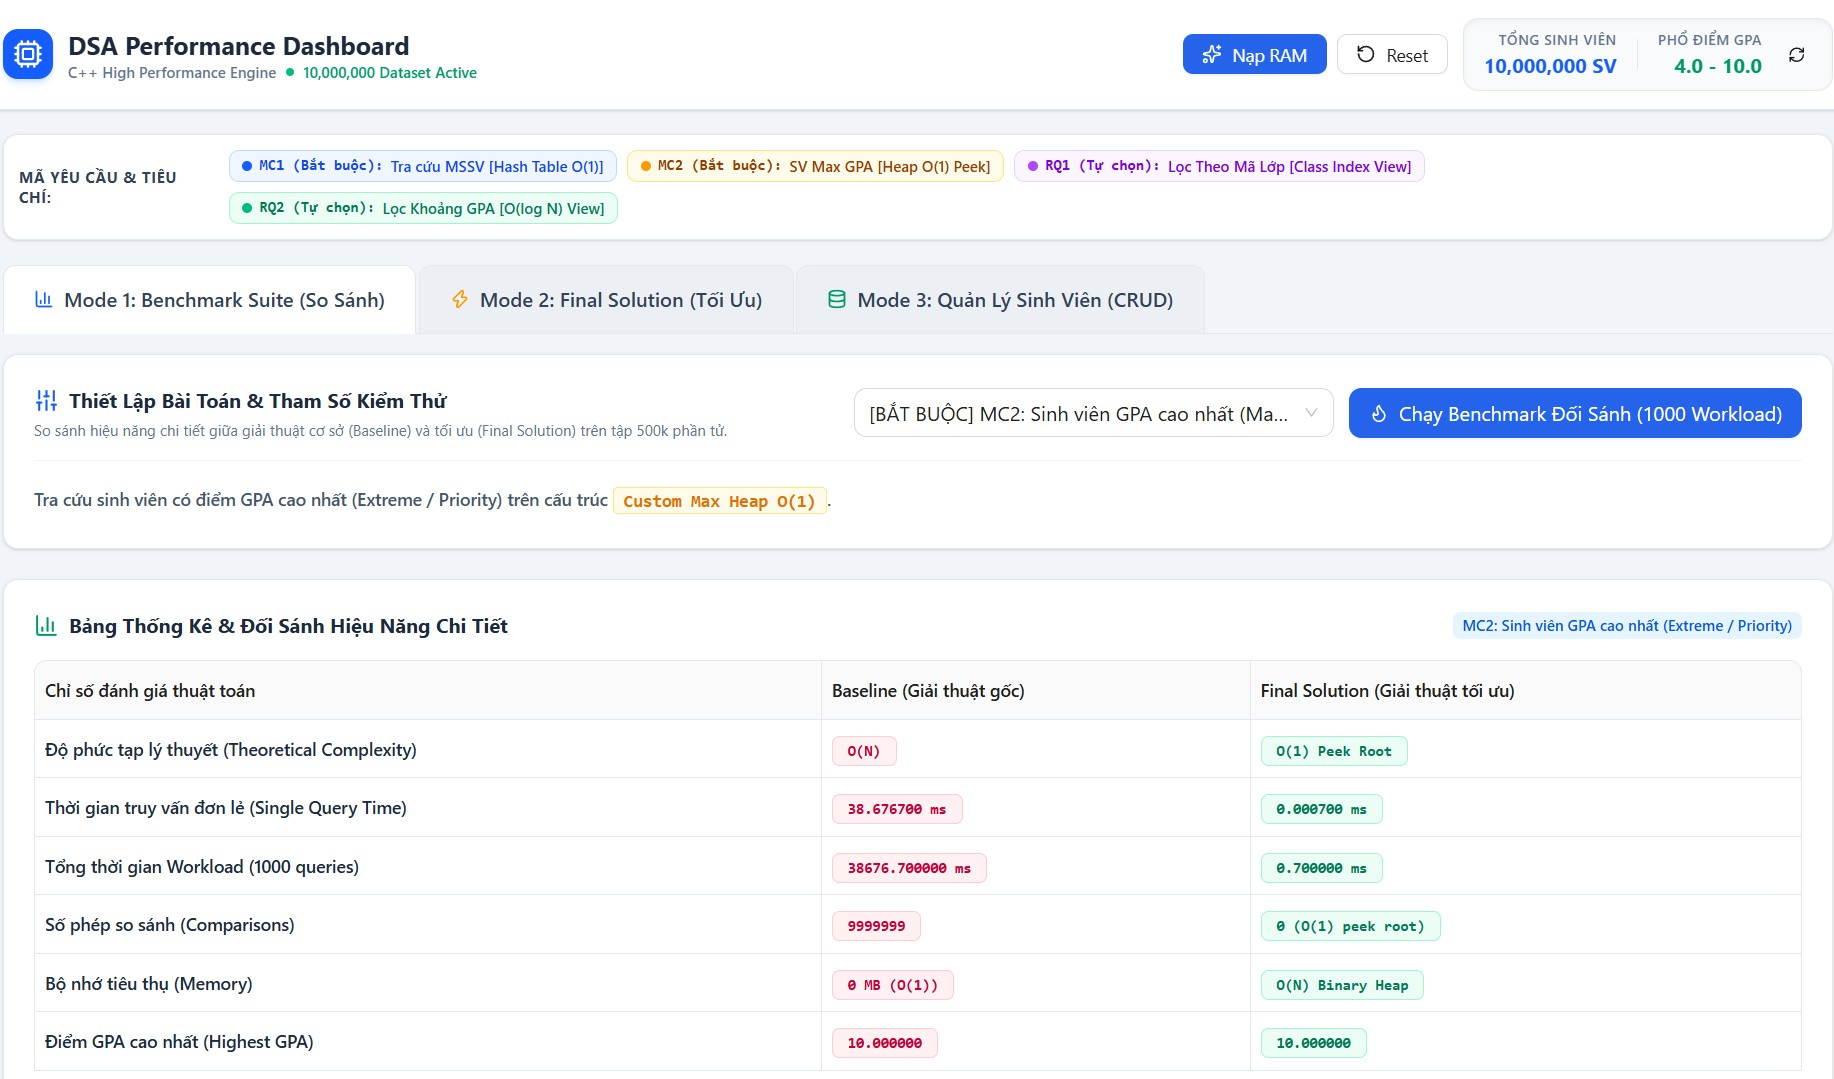
\includegraphics[width=0.68\textwidth]{benchmark_mc2_max_heap.jpeg}
\caption{Biểu đồ Benchmark MC2 trích xuất GPA cao nhất trên Max-Heap so với Baseline}
\label{fig:benchmark_mc2_max_heap}
\end{figure}

\subsubsection*{2.7.4. Kết quả đo thời gian thực thi các truy vấn tự phát hiện}
\addcontentsline{toc}{subsubsection}{2.7.4. Kết quả đo thời gian thực thi các truy vấn tự phát hiện}

Đối với yêu cầu RQ1 (Lọc danh sách sinh viên theo lớp), nhóm thực nghiệm kiểm chứng trên 4 trường hợp giao diện: lớp đầu dải ($C01$), lớp giữa dải ($C13$), lớp cuối dải ($C25$) và mã lớp không tồn tại ($C99$). Riêng bảng số C++ Core chọn lớp dày nhất trong tập 10M là \texttt{25KTP02}; lớp này có $52.649$ sinh viên. Baseline sao chép toàn bộ \texttt{Student} thỏa điều kiện, còn final dùng \texttt{ClassIndexViewResult}: chỉ mục \texttt{classId -> indexes} được build trước một lần, truy vấn chỉ còn lookup trung bình $O(1)$ và trả view không copy $K$ kết quả.

\begin{figure}[htbp]
\centering
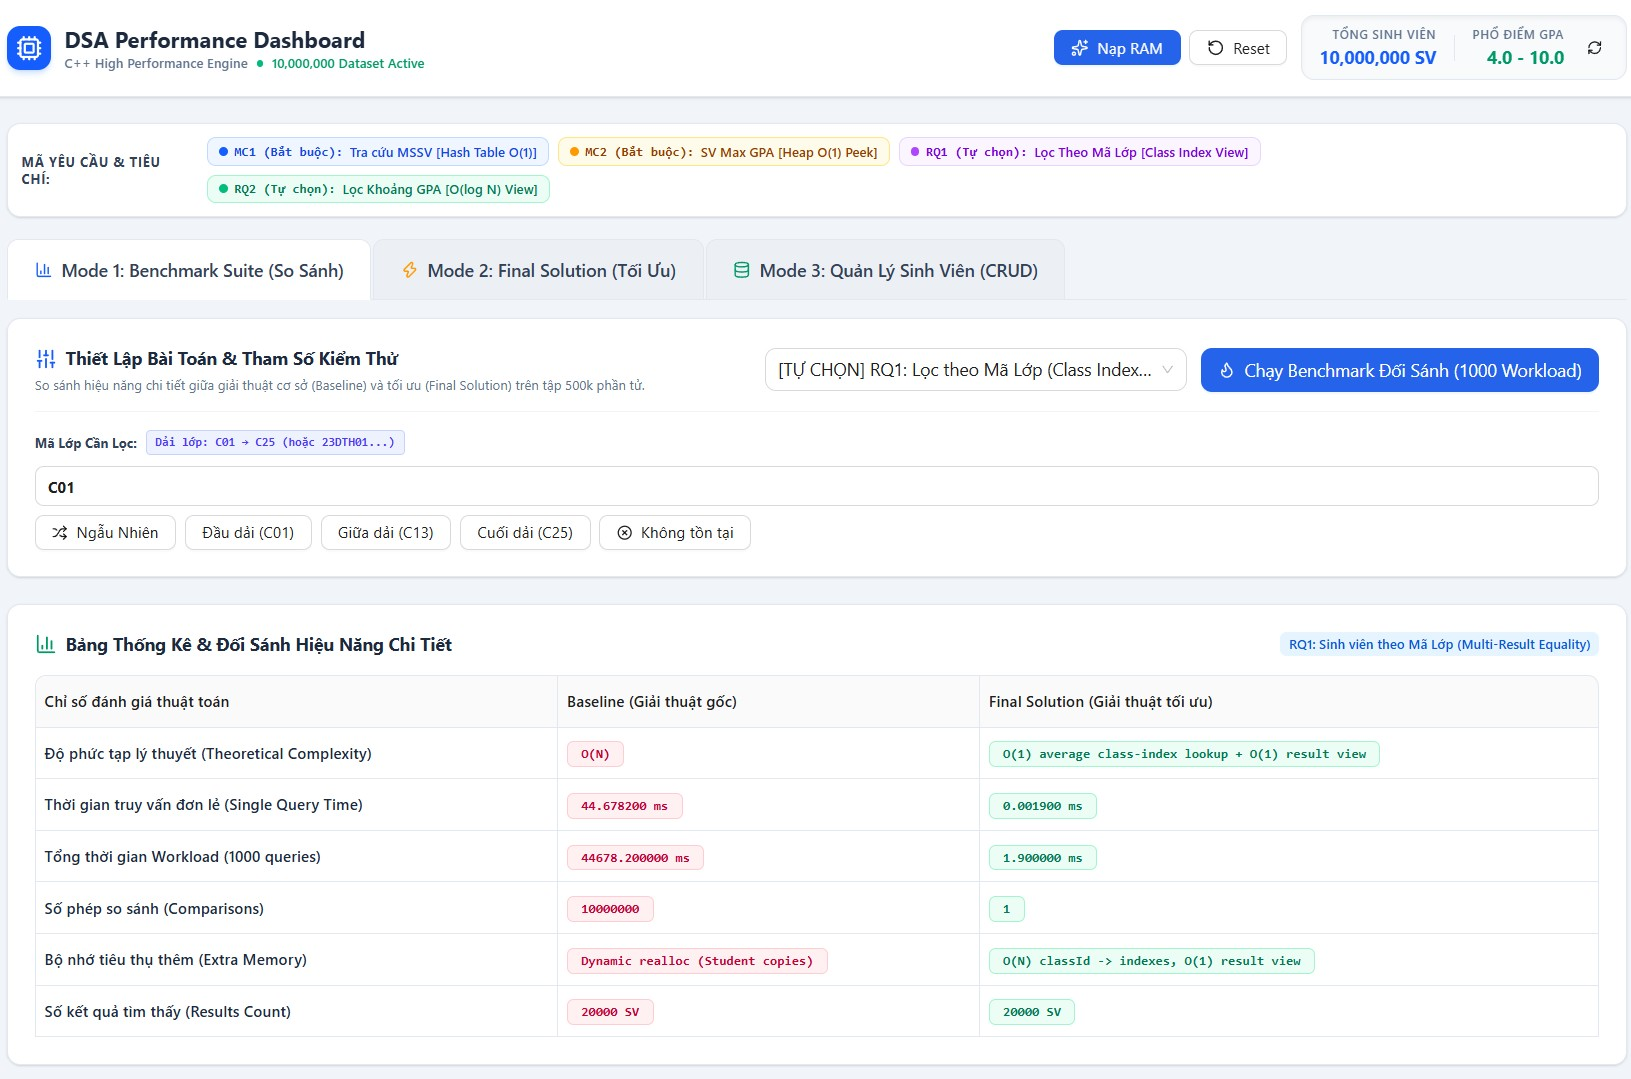
\includegraphics[width=0.56\textwidth]{rq1_lop_dau_dai.jpeg}
\caption{Benchmark RQ1 lọc danh sách sinh viên lớp C01 (Đầu dải)}
\label{fig:rq1_lop_dau_dai}
\end{figure}

\begin{figure}[htbp]
\centering
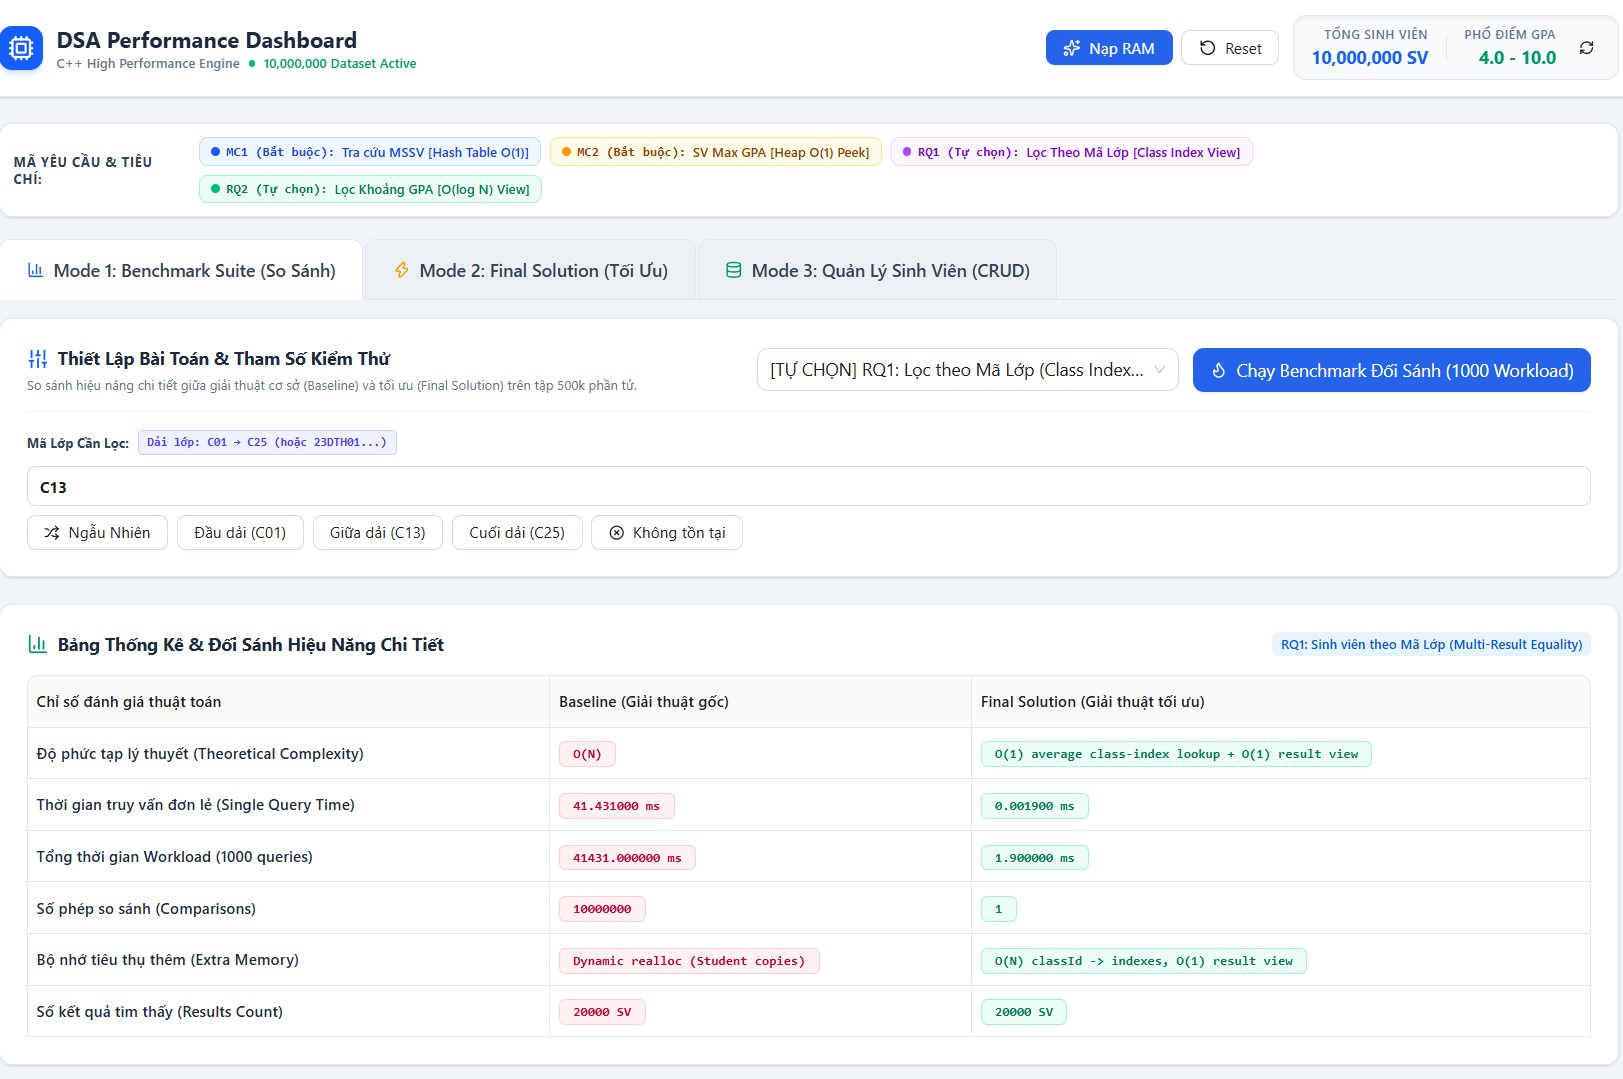
\includegraphics[width=0.56\textwidth]{rq1_lop_giua_dai.jpeg}
\caption{Benchmark RQ1 lọc danh sách sinh viên lớp C13 (Giữa dải)}
\label{fig:rq1_lop_giua_dai}
\end{figure}

Trong lần đo 10M, số phép so sánh giảm từ $10.000.000$ xuống $1$ lookup. Kết quả này phản ánh chi phí định vị chỉ mục và tạo view, chưa bao gồm chi phí materialize toàn bộ $52.649$ kết quả nếu tầng giao diện cần xuất hết.

\begin{figure}[htbp]
\centering
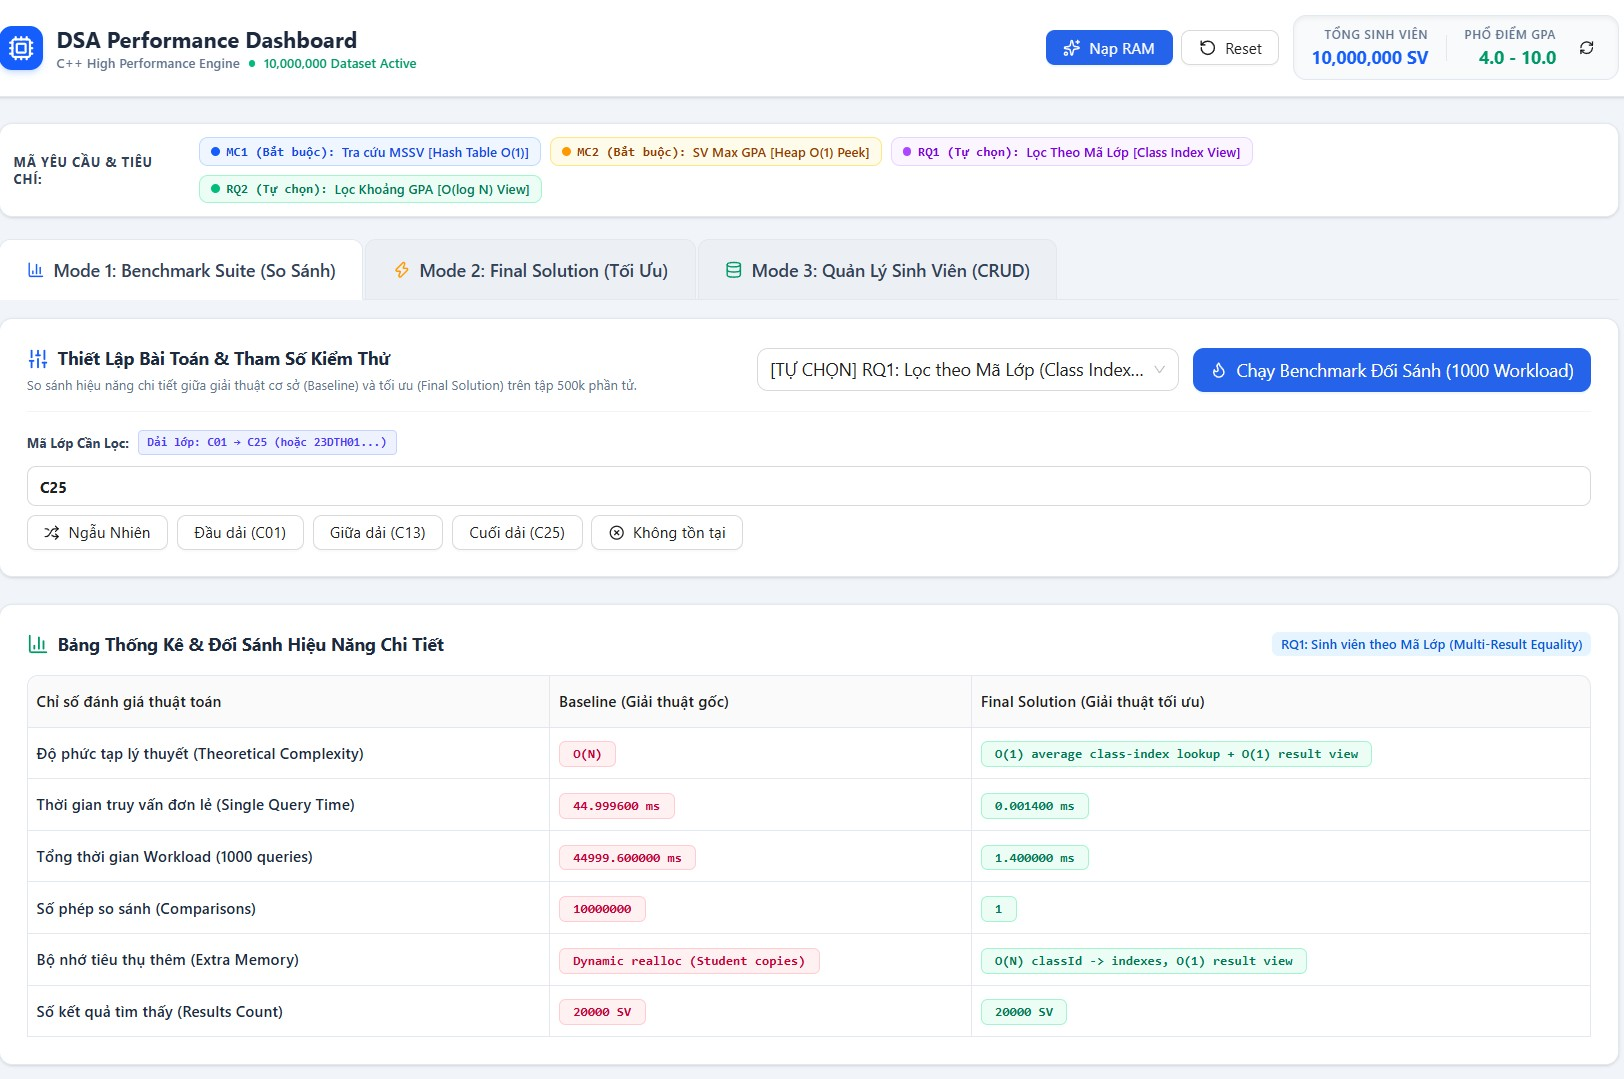
\includegraphics[width=0.56\textwidth]{rq1_lop_cuoi_dai.jpeg}
\caption{Benchmark RQ1 lọc danh sách sinh viên lớp C25 (Cuối dải)}
\label{fig:rq1_lop_cuoi_dai}
\end{figure}

\begin{figure}[htbp]
\centering
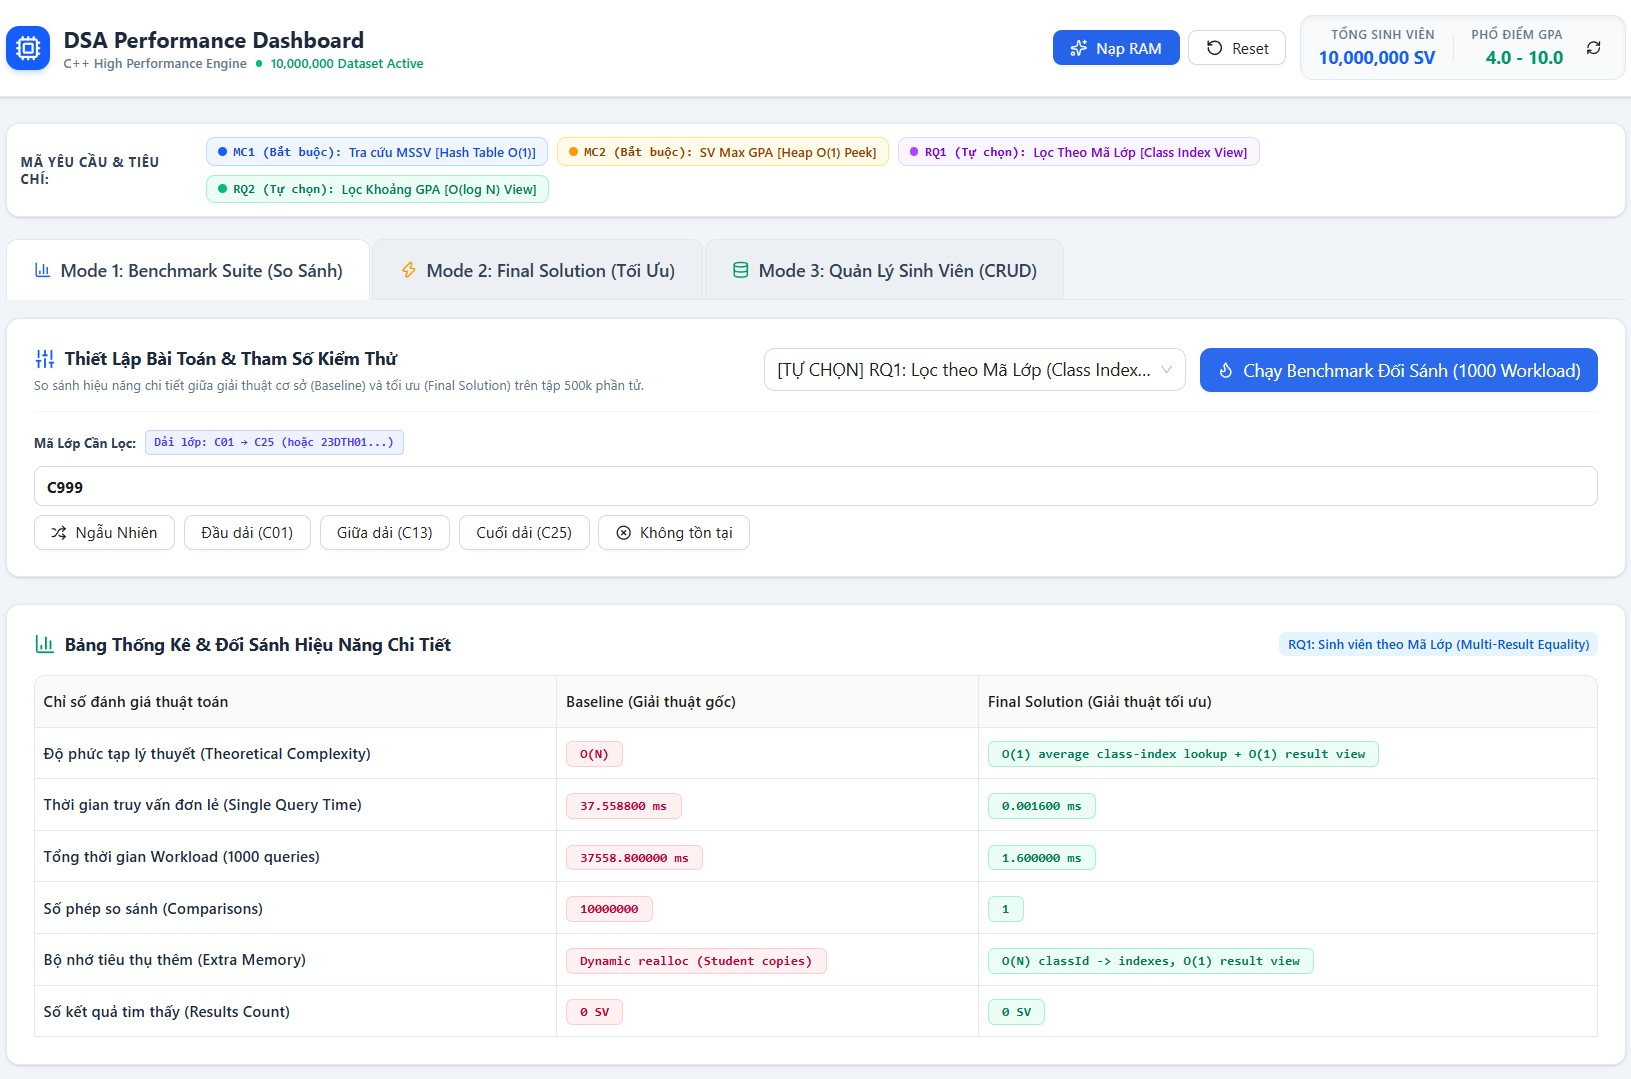
\includegraphics[width=0.56\textwidth]{rq1_lop_khong_ton_tai.jpeg}
\caption{Benchmark RQ1 khi tra cứu mã lớp không tồn tại}
\label{fig:rq1_lop_khong_ton_tai}
\end{figure}

Đối với yêu cầu RQ2 (bảng số đo khoảng GPA $[8.0, 10.0]$), Binary Search hai đầu biên giúp tìm nhanh vị trí bắt đầu và kết thúc trong $O(\log N)$. Sau khi tối ưu lại \texttt{SortedGpaFilter} theo hướng range view, code không còn sao chép $K$ bản ghi vào \texttt{vector<Student>} kết quả. Trong lần đo C++ Core 10M, khoảng này chứa $3.343.566$ sinh viên; LinearGPA mất median $331.479$ ms vì vừa quét toàn bộ $N$ vừa copy kết quả, còn SortedGPA chỉ cần $46$ so sánh biên và trả view trong khoảng $0.0001$ ms. Nếu tầng giao diện cần hiển thị dữ liệu, API chỉ dereference tối đa số phần tử preview cần gửi đi, nên chi phí hiển thị được tách khỏi chi phí tìm khoảng.

\begin{figure}[htbp]
\centering
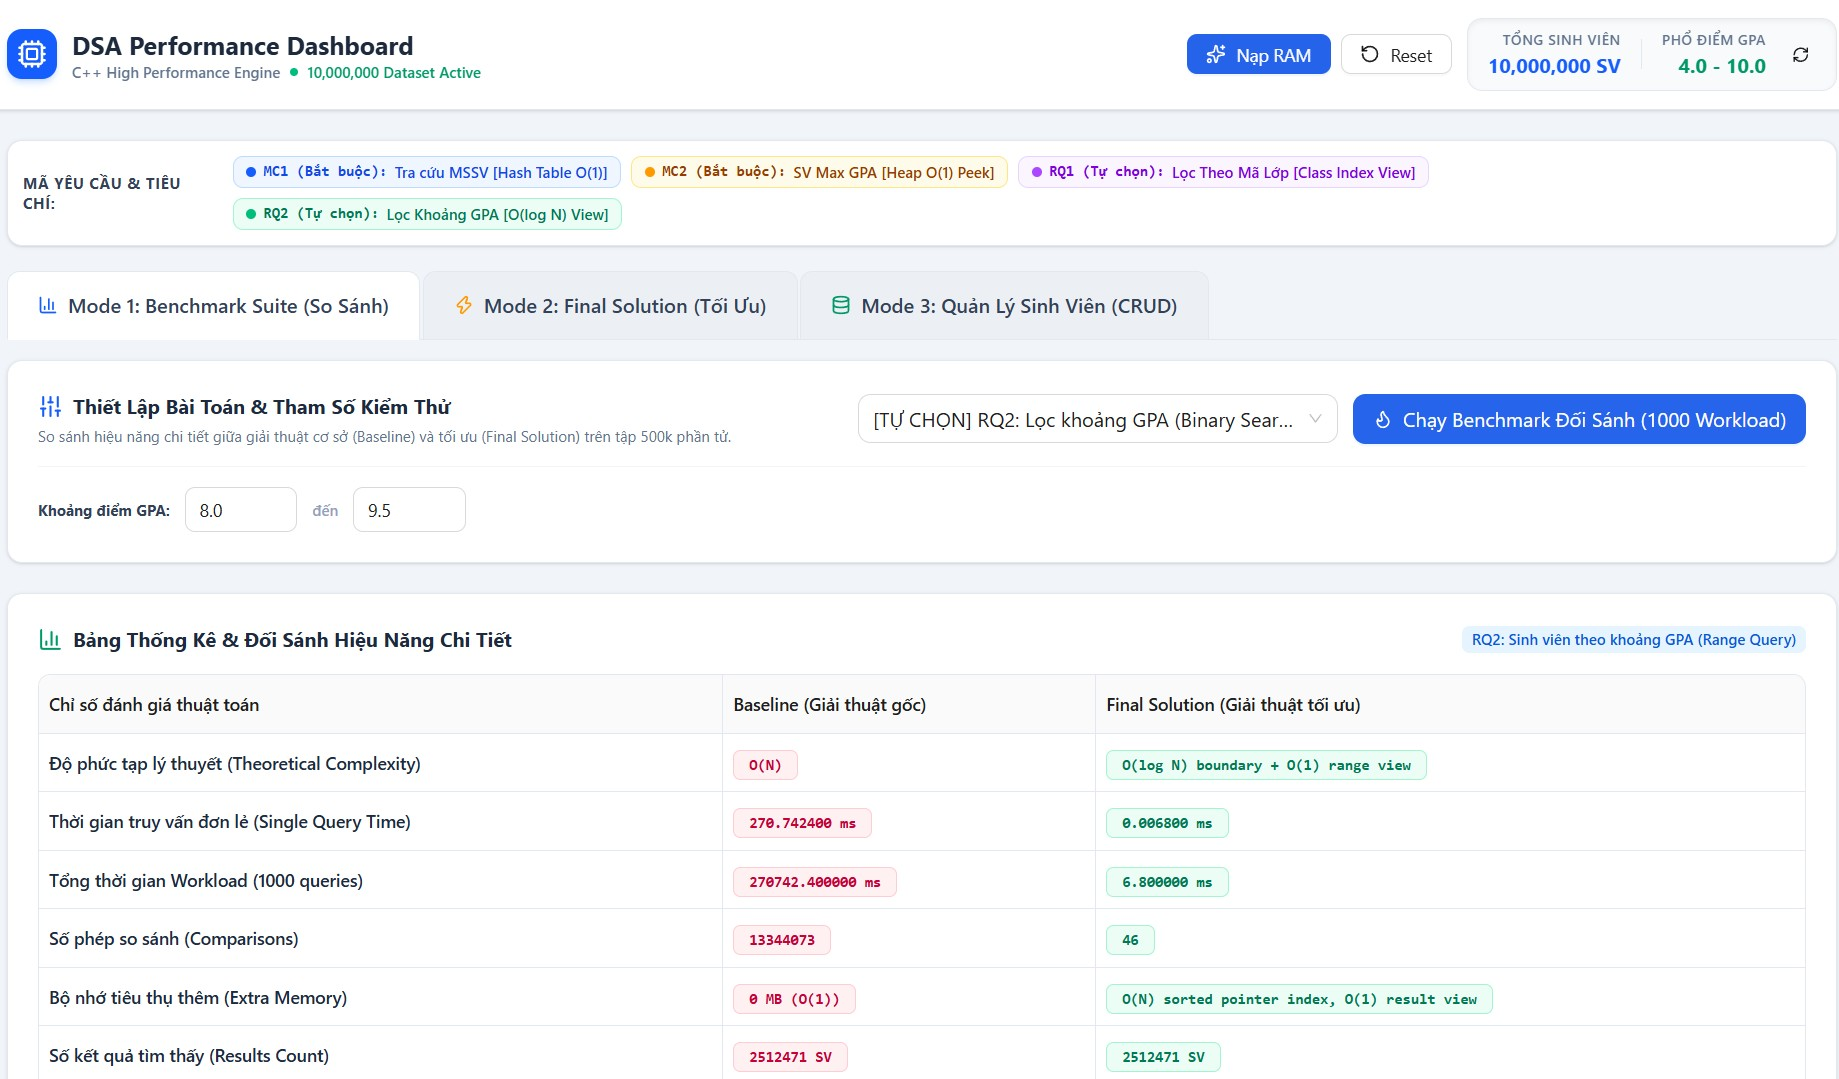
\includegraphics[width=0.68\textwidth]{benchmark_rq2_gpa_range.jpeg}
\caption{Dashboard minh họa truy vấn RQ2 với khoảng GPA [8.0, 9.5]; số liệu C++ Core trong Bảng \ref{tab:core_microbenchmark} sử dụng workload [8.0, 10.0]}
\label{fig:benchmark_rq2_gpa_range}
\end{figure}

\subsection*{2.8. Đối sánh hiệu năng thực nghiệm với lý thuyết và thuật toán tuyến tính}
\addcontentsline{toc}{subsection}{2.8. Đối sánh hiệu năng thực nghiệm với lý thuyết và thuật toán tuyến tính}

\subsubsection*{2.8.1. So sánh tốc độ Bảng băm đóng \texorpdfstring{($O(1)$)}{(O(1))} với Quét tuyến tính \texorpdfstring{($O(N)$)}{(O(N))}}
\addcontentsline{toc}{subsubsection}{2.8.1. So sánh tốc độ Bảng băm đóng \texorpdfstring{($O(1)$)}{(O(1))} với Quét tuyến tính \texorpdfstring{($O(N)$)}{(O(N))}}

Bảng tổng hợp đối sánh thực nghiệm thời gian thực thi giữa Bảng băm đóng và Thuật toán quét tuyến tính trên workload chính được trình bày chi tiết dưới đây:

\begin{table}[H]
\centering
\begingroup
\begin{singlespace}
\setlength{\tabcolsep}{3pt}
\renewcommand{\arraystretch}{1.3}
\begin{tabularx}{\textwidth}{|>{\raggedright\arraybackslash}m{2.7cm}|>{\centering\arraybackslash}m{2.2cm}|>{\centering\arraybackslash}m{2.2cm}|>{\centering\arraybackslash}m{2.1cm}|>{\raggedright\arraybackslash}X|}
\hline
\textbf{Workload} & \textbf{Linear} & \textbf{Closed Hash} & \textbf{Tăng tốc} & \textbf{Kết luận} \\ \hline
Build cấu trúc & --- & $399.537$ ms & --- & Chi phí dựng ban đầu $O(N)$ \\ \hline
$1.000$ truy vấn MSSV & $26424.51$ ms & $0.024$ ms & $\sim 1.09$M$\times$ & Hash lookup gần như hằng số sau build \\ \hline
Số bước kiểm tra & $\sim 5.228$B so sánh & $1.564$ probe & $\sim 3.34$M$\times$ & Khác biệt đến từ $O(N)$ và $O(1)$ trung bình \\ \hline
Tính đúng & $950/950$ hit + $50/50$ miss & $950/950$ hit + $50/50$ miss & Tương đương & Hai phương án đều trả đúng \\ \hline
\end{tabularx}
\end{singlespace}
\endgroup
\end{table}

Số liệu thực nghiệm khẳng định rằng trên cùng workload, thời gian thực thi của Bảng băm đóng nhỏ hơn rất nhiều so với Linear Search sau khi đã trả chi phí build ban đầu. Vì thời gian hash lookup ngắn hơn độ nhiễu của đồng hồ khi đo một lần đơn lẻ, nhóm đo theo batch $1.000$ truy vấn và dùng median của $9$ mẫu sau $5$ lượt warm-up để kết luận xu hướng $O(1)$ trung bình, không tuyên bố con số tuyệt đối như thời gian phản hồi UI.

\subsubsection*{2.8.2. So sánh tốc độ truy xuất Max-Heap \texorpdfstring{($O(1)$)}{(O(1))} với Quét tìm Max tuyến tính \texorpdfstring{($O(N)$)}{(O(N))}}
\addcontentsline{toc}{subsubsection}{2.8.2. So sánh tốc độ truy xuất Max-Heap \texorpdfstring{($O(1)$)}{(O(1))} với Quét tìm Max tuyến tính \texorpdfstring{($O(N)$)}{(O(N))}}

Trên tập dữ liệu thực nghiệm $10.000.000$ sinh viên, điểm mạnh của Max-Heap không nằm ở việc build nhanh hơn mọi phương án, mà ở chỗ sau khi build xong, thao tác đọc phần tử cực đại chỉ còn là truy cập phần tử gốc $O(1)$. Trong lần đo strict 10M, build heap mất median $1082.449$ ms; sau đó $100$ lần đọc cực trị chỉ mất median $0.016$ ms, trong khi $100$ lần quét tuyến tính mất median $3819.021$ ms. Chi phí khởi tạo vẫn là $O(N)$ theo Floyd Build Heap; vì vậy báo cáo tách riêng thời gian build và thời gian query để tránh hiểu nhầm rằng heap không cần trả chi phí chuẩn bị ban đầu.

\subsubsection*{2.8.3. Đánh giá chi tiết mức độ tiêu hao bộ nhớ RAM và hiệu ứng Cache}
\addcontentsline{toc}{subsubsection}{2.8.3. Đánh giá chi tiết mức độ tiêu hao bộ nhớ RAM và hiệu ứng Cache}

Toàn bộ hệ thống ưu tiên các cấu trúc mảng phẳng liên tục để có lợi cho tính định vị không gian của bộ đệm CPU Cache Line 64-byte. Các con số dưới đây là ước lượng lý thuyết từ \texttt{sizeof} trên nền tảng 64-bit, chưa bao gồm đầy đủ allocation riêng của \texttt{std::string} và overhead của container.

\textbf{Tập benchmark hiện tại -- $N = 10.000.000$:}

\textbf{Vùng lưu trữ sinh viên gốc:} $10.000.000 \times 104 \approx 1.040$ GB.

\textbf{Bảng băm đóng:} $M = 20.000.001$ ô, xấp xỉ $320$ MB.

\textbf{Mảng con trỏ sắp xếp GPA:} $10.000.000 \times 8 \approx 80$ MB.

\textbf{Chỉ mục ClassIndex cho RQ1:} Phần chỉ số \texttt{int} xấp xỉ $10.000.000 \times 4 \approx 40$ MB (chưa tính overhead container).

\textbf{Cây đống cực đại:} Bản sao \texttt{Student} xấp xỉ $1.040$ GB.

Tổng footprint lý thuyết phần thân các cấu trúc chính xấp xỉ $2.52$ GB, chưa bao gồm allocation riêng của \texttt{std::string}, bucket/metadata của container và overhead quản lý bộ nhớ của hệ điều hành.

Trong mô hình kiến trúc module hóa, các chỉ mục đọc nhiều ưu tiên mảng phẳng liên tục để tối ưu tính định vị không gian (Spatial Locality). Điểm cần lưu ý là footprint lý thuyết tính từ \texttt{sizeof} có thể cao hơn hoặc khác Working Set quan sát thực tế vì còn phụ thuộc vào allocation riêng của chuỗi, overhead container và việc các module có được giữ đồng thời ở dung lượng tối đa hay không. Sau tối ưu RQ1 và RQ2, \texttt{classIndex} chỉ lưu các chỉ số \texttt{int} theo lớp, còn \texttt{sortedStudents} chỉ còn là mảng con trỏ; vì vậy các truy vấn nhiều kết quả không còn tạo bản sao lớn của \texttt{Student} trong pha query.

\subsection*{2.9. Nhật ký gỡ lỗi (Debug Log) và tối ưu hóa giải thuật}
\addcontentsline{toc}{subsection}{2.9. Nhật ký gỡ lỗi (Debug Log) và tối ưu hóa giải thuật}

\subsubsection*{2.9.1. Ghi nhận lỗi phát sinh khi xử lý điều kiện dừng tìm kiếm trên Bảng băm}
\addcontentsline{toc}{subsubsection}{2.9.1. Ghi nhận lỗi phát sinh khi xử lý điều kiện dừng tìm kiếm trên Bảng băm}

Trong quá trình thực nghiệm ban đầu với Bảng băm đóng, nhóm phát hiện khi tra cứu một khóa MSSV không tồn tại trong hệ thống, nếu không giới hạn số bước dò tối đa thì trong trường hợp bảng đầy hoặc vòng lặp chỉ số có sai lệch, hàm có thể lặp quá mức cần thiết. Nhóm đã hoàn thiện giải thuật: vòng dò dừng ngay lập tức khi bắt gặp ô chưa chiếm (\texttt{!table[index].occupied}) đầu tiên, đồng thời giới hạn số lần duyệt tối đa không vượt quá kích thước bảng $M$, đảm bảo thao tác tìm kiếm thất bại luôn kết thúc nhanh chóng và an toàn.

\subsubsection*{2.9.2. Tối ưu hóa cấp phát bộ nhớ và bảo toàn con trỏ trong Bulk Load}
\addcontentsline{toc}{subsubsection}{2.9.2. Tối ưu hóa cấp phát bộ nhớ và bảo toàn con trỏ trong Bulk Load}

Trong quá trình nạp dữ liệu quy mô lớn, việc \texttt{std::vector} tự động mở rộng dung lượng nhiều lần sẽ phát sinh chi phí sao chép dữ liệu và có thể làm thay đổi địa chỉ bộ nhớ của các phần tử \texttt{Student}. Lệnh \texttt{reserve()} giúp giảm số lần tái cấp phát và giữ ổn định vùng dữ liệu gốc trước khi xây dựng các chỉ mục lưu con trỏ như \texttt{HashTable} và \texttt{SortedGpaFilter}. Riêng MaxHeap không phụ thuộc vào con trỏ về vùng gốc vì chủ động xây dựng bản sao \texttt{Student} nội bộ. Đánh đổi của cách cấp phát trước là có thể giữ capacity lớn hơn nhu cầu tức thời nếu tập dữ liệu thực nghiệm nhỏ hơn mốc thiết kế.

\subsection*{2.10. Tuyên bố Trách nhiệm Giải trình về Sử dụng AI và Liêm chính Học thuật (AI-Audit Log)}
\addcontentsline{toc}{subsection}{2.10. Tuyên bố Trách nhiệm Giải trình về Sử dụng AI và Liêm chính Học thuật (AI-Audit Log)}

Nhằm tuân thủ quy định về Liêm chính học thuật và Chuẩn mực nghiên cứu khoa học của Trường Đại học Công nghệ Kỹ thuật TP. Hồ Chí Minh, nhóm tác giả công khai nhật ký sử dụng các công cụ Trí tuệ Nhân tạo tạo sinh (GenAI / LLMs) trong quá trình thực hiện đề tài:

\begin{table}[H]
\centering
\begingroup
\small
\begin{singlespace}
\setlength{\tabcolsep}{3.5pt}
\renewcommand{\arraystretch}{1.15}
\begin{tabularx}{\textwidth}{|>{\raggedright\arraybackslash}p{2.6cm}|>{\raggedright\arraybackslash}p{3.8cm}|>{\raggedright\arraybackslash}X|}
\hline
\textbf{Hạng mục} & \textbf{Mức độ \& Công cụ AI} & \textbf{Trách nhiệm và Đóng góp của Nhóm Sinh viên} \\ \hline
Thiết kế CTDL & Gợi ý cú pháp C++20 và mẫu biểu diễn struct. & Nhóm trực tiếp thiết kế Closed Hash Table, Floyd Max-Heap, kiến trúc 3 tầng và mảng dữ liệu sắp xếp. \\ \hline
Cài đặt Thuật toán & Hỗ trợ rà soát cú pháp và tối ưu vòng lặp. & Tự cài đặt FNV-1a, Linear Probing, Floyd Build-Heap, iterative heapifyDown và Binary Search 2 đầu biên; triển khai Class Index View cho RQ1 bằng \texttt{std::unordered\_map<string, vector<int>>}; sử dụng \texttt{std::sort} dựng mảng GPA ban đầu. \\ \hline
Thực nghiệm Benchmark & Hỗ trợ sinh mã kịch bản đo thời gian \texttt{std::chrono}. & Nhóm trực tiếp thực thi đo đạc trên máy tính cá nhân với tập dữ liệu hiện tại $10.000.000$ sinh viên, dùng $5$ lượt warm-up và $9$ mẫu đo để ghi nhận số liệu thực tế. \\ \hline
Giao diện Web/API & Hỗ trợ khung thành phần giao diện React/Next.js. & Nhóm trực tiếp xây dựng API Bridge C++, binding dữ liệu và kiểm thử trải nghiệm người dùng. \\ \hline
Báo cáo LaTeX & Hỗ trợ căn chỉnh bảng biểu, phản biện tính nhất quán và định dạng. & Nhóm trực tiếp biên soạn nội dung học thuật, phân tích kết quả và kiểm duyệt toàn bộ báo cáo. \\ \hline
\end{tabularx}
\end{singlespace}
\endgroup
\caption{Nhật ký giải trình minh bạch việc sử dụng công cụ AI (AI-Audit Log)}
\label{tab:ai_audit_log}
\end{table}

Cam kết liêm chính học thuật: Toàn bộ thành viên trong nhóm khẳng định các cấu trúc dữ liệu, thuật toán và giải pháp kiến trúc trong báo cáo đều do nhóm trực tiếp nghiên cứu, lập trình và kiểm nghiệm thực tế. Công cụ AI được sử dụng để hỗ trợ rà soát cú pháp, phản biện tính nhất quán kỹ thuật và chuẩn hóa định dạng LaTeX. Nhóm sinh viên trực tiếp quyết định thiết kế, kiểm tra mã nguồn, thực thi benchmark và chịu trách nhiệm trước Hội đồng chấm thi về tính xác thực của công trình.

% ==============================================================================
% KẾT LUẬN VÀ BÀI HỌC KINH NGHIỆM
% ==============================================================================
\newpage
\section*{PHẦN KẾT LUẬN VÀ BÀI HỌC KINH NGHIỆM}
\addcontentsline{toc}{section}{PHẦN KẾT LUẬN VÀ BÀI HỌC KINH NGHIỆM}

\subsection*{1. Kết luận tổng quan về dự án}
\addcontentsline{toc}{subsection}{1. Kết luận tổng quan về dự án}

Trải qua quá trình nghiên cứu và phát triển, nhóm đã hoàn thiện hệ thống quản lý cơ sở dữ liệu sinh viên quy mô lớn và kiểm thử thực nghiệm trực tiếp tại mốc $10.000.000$ bản ghi, qua đó đánh giá khả năng vận hành ở quy mô lớn cũng như bài toán cân bằng giữa tốc độ xử lý tức thì và giới hạn tài nguyên phần cứng.

Việc tự tay cài đặt hai cấu trúc dữ liệu cốt lõi cùng các thuật toán trọng tâm giúp nhóm nắm vững bản chất hoạt động ở cấp độ bộ nhớ. Các kết quả thực nghiệm với Bảng băm đóng kết hợp FNV-1a, Max-Heap, Class Index View và Mảng con trỏ sắp xếp cho kết quả phù hợp với xu hướng được dự đoán từ phân tích độ phức tạp $O(1)$, $O(N)$ và $O(\log N)$ cho range view. Kết quả trên tập $10.000.000$ bản ghi là cơ sở để nhóm đánh giá khả năng đáp ứng ở quy mô lớn.

Đặc biệt, mô hình kiến trúc phân tầng kết hợp chiến lược tổ chức dữ liệu mảng phẳng liên tục cho thấy hệ thống có thể vận hành ổn định trong giới hạn tài nguyên bộ nhớ RAM của máy thử nghiệm. Báo cáo ưu tiên sử dụng ước lượng footprint lý thuyết ở Mục 2.8.3 để trình bày chi phí bộ nhớ, vì Working Set quan sát bởi hệ điều hành tại từng thời điểm có thể khác với tổng vùng nhớ được cấp phát/committed. Đây là cơ sở thực nghiệm giúp nhóm kết nối giữa lý thuyết thuật toán và các kỹ thuật lập trình hệ thống hiệu năng cao.

\subsection*{2. Bài phản tư cá nhân của 4 thành viên (Individual Reflections - D7)}
\addcontentsline{toc}{subsection}{2. Bài phản tư cá nhân của 4 thành viên (Individual Reflections - D7)}

\subsubsection*{2.1. Phản tư của sinh viên Bùi Tấn Phát (MSSV: 25110289)}
\addcontentsline{toc}{subsubsection}{2.1. Phản tư của sinh viên Bùi Tấn Phát (MSSV: 25110289)}
Ở vai trò nhóm trưởng, em chịu trách nhiệm điều phối tiến độ chung, phân công nhiệm vụ và tổng hợp báo cáo kỹ thuật của nhóm. Về mặt kỹ thuật, nhiệm vụ chính của em là cài đặt Bảng băm đóng với kích thước động $M = 2N + 1$ để phục vụ yêu cầu tra cứu MC1. Trên tập benchmark $10.000.000$ bản ghi, bảng có $20.000.001$ ô. Trong giai đoạn đầu kiểm thử với trường hợp mã sinh viên không tồn tại, em gặp sự cố hàm tìm kiếm bị lặp quá số bước cần thiết do chưa chặn chặt chẽ điều kiện dừng của vòng dò tuyến tính. Sau khi rà soát cơ chế của bảng băm tĩnh hai trạng thái, em đã cập nhật điều kiện dừng ngay khi gặp ô trống đầu tiên (\texttt{!occupied}) hoặc khi số bước dò chạm ngưỡng kích thước bảng $M$, nhờ đó hàm tìm kiếm luôn trả về \texttt{nullptr} an toàn mà không phát sinh vòng lặp vô tận. Qua phần này, em hiểu sâu sắc về công thức kỳ vọng số bước dò của Knuth và tầm quan trọng của việc kiểm soát hệ số tải $\alpha \approx 0.50$ trong thực tế. Quá trình làm đồ án giúp em nâng cao tư duy quản lý dự án, kỹ năng phân bổ công việc và phối hợp làm việc nhóm hiệu quả. Em cam kết toàn bộ phần điều phối, cài đặt và kiểm thử Bảng băm thuộc phạm vi của mình được thực hiện trung thực.

\subsubsection*{2.2. Phản tư của sinh viên Nguyễn Phan Thành Tiến (MSSV: 25110361)}
\addcontentsline{toc}{subsubsection}{2.2. Phản tư của sinh viên Nguyễn Phan Thành Tiến (MSSV: 25110361)}
Phần em đảm nhận trong đồ án là xây dựng Max-Heap tự cài đặt để trích xuất sinh viên có GPA cao nhất cho yêu cầu MC2. Quyết định kỹ thuật quan trọng nhất của em là chuyển giải thuật \texttt{heapifyDown} từ dạng đệ quy sang vòng lặp \texttt{while} nhằm loại bỏ chi phí gọi hàm và trực tiếp kiểm soát chỉ số nút con trên mảng một chiều. Khó khăn thực tế em xử lý là trường hợp nhiều sinh viên cùng đạt mức điểm cực đại $10.0$; em đã thiết kế hàm so sánh ưu tiên kết hợp cả điểm GPA và so sánh chuỗi MSSV theo thứ tự từ điển để bảo đảm tính tất định ở nút gốc. Qua trải nghiệm này, em nắm vững thuật toán Floyd Build Heap $O(N)$ và cách tổ chức cây nhị phân hoàn chỉnh trên mảng liên tục. Em cam kết toàn bộ mã nguồn Max-Heap và dữ liệu thực nghiệm MC2 do em trực tiếp thực hiện.

\subsubsection*{2.3. Phản tư của sinh viên Ngô Đức Thành (MSSV: 25110335)}
\addcontentsline{toc}{subsubsection}{2.3. Phản tư của sinh viên Ngô Đức Thành (MSSV: 25110335)}
Nhiệm vụ trọng tâm của em trong đồ án là phụ trách yêu cầu tự phát hiện \textbf{RQ1} (Lọc danh sách sinh viên theo Lớp học phần). Để tối ưu hóa hiệu năng trên tập dữ liệu $10.000.000$ bản ghi, em đã nghiên cứu và trực tiếp cài đặt cấu trúc \texttt{ClassIndexFilter} theo cơ chế Class Index View (\texttt{std::unordered\_map<string, vector<int>>}). Giải pháp này cho phép hệ thống chỉ cần duyệt mảng dữ liệu một lần duy nhất lúc khởi động để gom nhóm các chỉ số sinh viên theo mã lớp với chi phí $O(N)$, sau đó mỗi truy vấn lọc theo lớp chỉ mất thời gian trung bình $O(1)$ để trích xuất view con trỏ chỉ mục mà không phải sao chép bất kỳ đối tượng \texttt{Student} nào. Thách thức lớn nhất em đã vượt qua là kiểm soát dung lượng bộ nhớ của chỉ mục lớp và xử lý an toàn các trường hợp mã lớp không tồn tại hoặc lớp có số lượng sinh viên lớn khi chạy tải benchmark. Qua đồ án, em nắm vững kỹ thuật lập chỉ mục phụ (Secondary Indexing) và phương pháp thiết kế cấu trúc dữ liệu không sao chép (Zero-copy View) trong C++. Em cam kết toàn bộ thuật toán và kết quả kiểm thử RQ1 thuộc phần việc của mình đều trung thực.

\subsubsection*{2.4. Phản tư của sinh viên Đặng Đoàn Minh Khang (MSSV: 25110227)}
\addcontentsline{toc}{subsubsection}{2.4. Phản tư của sinh viên Đặng Đoàn Minh Khang (MSSV: 25110227)}
Nhiệm vụ của em trong đồ án là phụ trách yêu cầu tự phát hiện \textbf{RQ2} (Lọc sinh viên theo khoảng điểm GPA) kết hợp thiết kế kiến trúc tổng thể của hệ thống. Với RQ2, em xây dựng module \texttt{SortedGpaFilter} sử dụng mảng con trỏ \texttt{vector<const Student*>} sắp xếp theo GPA tăng dần và tự cài đặt thuật toán Tìm kiếm Nhị phân 2 đầu biên (\textit{Lower Bound} và \textit{Upper Bound}) để định vị chính xác khoảng giá trị $[\text{minGPA}, \text{maxGPA}]$ trong thời gian logarit $O(\log N)$. Khó khăn lớn nhất em đã xử lý là các trường hợp biên của dải điểm khi nhiều sinh viên chạm đúng giá trị cận trên \texttt{maxGPA}; em đã hoàn thiện điều kiện so sánh $\le \text{maxGPA}$ và tối ưu kết quả trả về dưới dạng range view \texttt{GpaRangeViewResult} để tránh sao chép mảng sinh viên. Bên cạnh đó, em đảm nhận vai trò thiết kế kiến trúc phân tầng 3 tầng, quy trình nạp dữ liệu hàng loạt (Bulk Load) sử dụng \texttt{reserve()} để chống phân mảnh bộ nhớ, và xây dựng tầng API Bridge kết nối C++ DSA Core với Web Dashboard trực quan. Quá trình làm đồ án giúp em nâng cao tư duy thiết kế giải thuật kết hợp kiến trúc hệ thống hiệu năng cao. Em cam kết toàn bộ phần việc thuộc phạm vi của mình được thực hiện trung thực.

% ==============================================================================
% TÀI LIỆU THAM KHẢO
% ==============================================================================
\newpage
\section*{TÀI LIỆU THAM KHẢO}
\addcontentsline{toc}{section}{TÀI LIỆU THAM KHẢO}

\begin{enumerate}[label={[\arabic*]}, leftmargin=*, itemsep=6pt, parsep=0pt, topsep=4pt]
    \item Thomas H. Cormen, Charles E. Leiserson, Ronald L. Rivest, and Clifford Stein (2022), \textit{Introduction to Algorithms (CLRS)}, 4th Edition, The MIT Press \& McGraw-Hill, Cambridge, Massachusetts. (Trọng tâm: Chương 6 -- Heapsort và Hàng đợi ưu tiên; Chương 11 -- Bảng băm và Kỹ thuật giải quyết đụng độ Open Addressing).
    
    \item Donald E. Knuth (1998), \textit{The Art of Computer Programming, Volume 3: Sorting and Searching}, 2nd Edition, Addison-Wesley Professional, Reading, Massachusetts. (Trọng tâm: Mục 6.4 -- Hashing, Giải thuật Dò tuyến tính Linear Probing và Phân tích toán học về cụm sơ cấp).
    
    \item Robert Sedgewick and Kevin Wayne (2011), \textit{Algorithms}, 4th Edition, Addison-Wesley Professional, Boston. (Trọng tâm: Chương 2.4 -- Priority Queues; Chương 3.4 -- Hash Tables; Phân tích thực nghiệm cấu trúc dữ liệu trên bộ nhớ chính).
    
    \item Mark Allen Weiss (2014), \textit{Data Structures and Algorithm Analysis in C++}, 4th Edition, Pearson Education, Upper Saddle River, New Jersey. (Trọng tâm: Cài đặt Cấu trúc Dữ liệu tối ưu hiệu năng và Kỹ thuật quản lý con trỏ bản ghi).
    
    \item Robert W. Floyd (1964), ``Algorithm 245: Treesort 3'', \textit{Communications of the ACM (CACM)}, Tập 7, Số 12, tr. 701, DOI: 10.1145/355588.365103. (Công trình gốc đề xuất giải thuật vun đống Floyd Build-Heap với độ phức tạp tuyến tính $O(N)$ từ dưới lên).
    
    \item Glenn Fowler, Landon Curt Noll, and Phong Vo (2011), ``Fowler--Noll--Vo Hash Function (FNV-1a)'', \textit{Internet Engineering Task Force (IETF) Specification Draft}, Silicon Graphics \& Cisco Systems. (Đặc tả giải thuật hàm băm FNV-1a 64-bit với các hằng số nguyên tố FNV\_PRIME và FNV\_OFFSET\_BASIS).
    
    \item Bjarne Stroustrup (2013), \textit{The C++ Programming Language}, 4th Edition, Addison-Wesley Professional, Boston. (Trọng tâm: Mô hình bộ nhớ RAM, Tổ chức Layout đối tượng phẳng, Kỹ thuật tránh phân mảnh và Quản lý tài nguyên RAII).
    
    \item Ulrich Drepper (2007), ``What Every Programmer Should Know About Memory'', \textit{Red Hat Technical Whitepaper}, tr. 1--114. (Phân tích chuyên sâu về kiến trúc phân cấp bộ nhớ, đường truyền Bus, bộ đệm Cache L1/L2/L3, hiện tượng Cache Line Miss và phương pháp tối ưu hóa dữ liệu liền kề Contiguous Memory Layout).
    
    \item ISO/IEC 14882:2020 (2020), \textit{Programming Languages --- C++ (International Standard ISO/IEC C++20 Specification)}, International Organization for Standardization, Geneva, Switzerland. (Chuẩn ngôn ngữ lập trình C++20 và Đặc tả hệ thống thư viện thời gian chính xác cao \texttt{std::chrono}).
    
    \item Đinh Bá Tiến, Trương Anh Hoàng, Trần Hạnh Nhi (2020), \textit{Giáo trình Cấu trúc Dữ liệu và Giải thuật}, NXB Đại học Quốc gia TP. Hồ Chí Minh, TP. Hồ Chí Minh.
    
    \item Nguyễn Trung Trực (2018), \textit{Cấu trúc Dữ liệu và Giải thuật trong C/C++}, NXB Khoa học và Kỹ thuật, Hà Nội.
    
    \item Bộ môn Công nghệ Phần mềm, Khoa Công nghệ Thông tin (2024), \textit{Đề cương chi tiết và Hướng dẫn thực hành học phần Cấu trúc Dữ liệu và Giải thuật (Mã lớp học phần: DASA230179\_03)}, Trường Đại học Công nghệ Kỹ thuật TP. Hồ Chí Minh.
\end{enumerate}

\end{document}




